% You may wish to use some of the following options of the iitthesis
% package:
%
% fullpageDraft      avoid the margins necessary for proper binding and
%   just view or print a draft.
% beforeDefense      make the personal acknowledgements invisible;
%   use this to print the copies you submit initially to the grad school
%   for sending to the opponent panel, i.e. thesis readers (who shouldn't
%   see those parts). For the final submission, after having successfully
%   defended - drop this option.
% noabbrevs          avoid generation of a notation & abbreviations list
%
% Additionally, you must specify the degree for which you're writing
% your thesis (MSc/PhD/MArch etc.)
%
\documentclass[MSc,beforeDefense]{misc/iitthesis}


% Definitions of info fields for the thesis - subject, advisor,
% faculty, acknowledgements, etc. etc. The thesis-fields file
% contains Hebrew text, and should use the UTF-8 character set
% encoding (not iso-8859-8-i or windows codepage 1255).
% This file contains definitions of various fields used
% in various places throughout the thesis (in the title
% pages mostly). Whatever isn't define here has some
% default (and usually irrelevant) text.

\authorEnglish{Ohad Levy-Or}
\authorHebrew{אוהד לוי-אור}

\titleEnglish{Novel Class of Expected Value Bounds and Applications in Belief Space Planning}
\titleHebrew{משפחה חדשה של חסמים על תוכלת ושימושים בתכנון תחת אי וודעות}

\disciplineEnglish{Robotics and Autonomy}
\disciplineHebrew{רובוטיקה ואוטונומיה}

\supervisionEnglish{This research was carried out under the supervision of Prof. Vadim Indelman, in the Faculty of Aerospace Engineering.}
\supervisionHebrew{המחקר בוצע בהנחייתו של פרופסור ואדים אינדלמן, בפקולטה להנדסת אוירונוטיקה וחלל.}

\GregorianDateEnglish{August 2024}
\GregorianDateHebrew{אוגוסט \textenglish{2024}}
\JewishDateEnglish{Av 5784}
\JewishDateHebrew{אב התשפ"ד}

\financialAcknowledgementEnglish{The Technion's funding of this research is hereby acknowledged.}
\financialAcknowledgementHebrew{הכרת תודה מסורה לטכניון על מימון מחקר זה.}

\publicationInfoEnglish{%

Some results in this thesis have been published as articles by the author and research collaborators in conferences and journals during the course of the author's doctoral research period, the most up-to-date versions of which being:

\butcheredbibliography{front/pubinfo.bib}
}

\publicationInfoHebrew{%

חלק מן התוצאות בחיבור זה פורסמו כמאמרים מאת המחבר ושותפיו למחקר בכנסים ובכתבי-עת במהלך תקופת מחקר הדוקטורט של המחבר, אשר גרסאותיהם העדכניות ביותר הינן:%

\begin{otherlanguage}{english}%
\butcheredbibliography{front/pubinfo.bib}
\end{otherlanguage}%
}

\addbibresource{back/general.bib}
% \thesisbibstyle{trad-alpha}


% Personal acknowledgements (are only used for the post-exam
% version)
\personalAcknowledgementEnglish{
I would like to thank my advisor, Vadim Indelman for being a guiding hand in all my research related endeavors.\\
I would like to thank my supportive wife, Tash, for being a shining light in the difficult times, both in research and otherwise.
}

\personalAcknowledgementHebrew{
טש שלי, תודה על הייותך לי אור בימים אפרוריים.
}


% A separate file for the abstract - in English and in Hebrew, so
% you must make sure it's also in the UTF-8 character set encoding.
%
% This file contains the abstract part of your thesis - in English and
% in Hebrew (within \abstractEnglish and \abstractHebrew respectively).
%
% Notes:
% - This file uses the UTF-8 character set encoding for the Hebrew
%   text not to get garbled. Keep it that way.
% - Assuming your thesis is mainly in English, Graduate School
%   regulations mandate the following lengths for the abstracts:
%
%      Language    Min. Length   Max. Length
%     ---------------------------------------
%      English       200 words     500 words
%      Hebrew        500 words   2,000 words
%
%   so that the Hebrew abstract typically has some content from
%   the English introduction and an overview of the results, not
%   present in the English; it is not just a translation.

\abstractEnglish{

Planning under uncertainty in partially observable domains, often formulated as \glspl{pomdp}, is an exceedingly difficult problem. Finding the globally optimal solution is intractable for all but the smallest problems as it requires reasoning about realization of the many random variables of the problem. Thus, tractable bounds with formal guarantees are attractive alternative to finding a globally optimal solution. In this paper, motivated by this line of reasoning, we formulate and prove novel probability theory bounds. First, we bound the expectation with respect to the partial expectation (seen to be directly proportional to the conditional expectation) and show that this is a generalization of the Markov inequality. Second, by merging our novel inequalities with Hoeffding's inequality, we compose an additional novel bound, which allows for bounding expectations with respect to estimators of partial expectations. Finally, we apply these bounds to the context of planning; we prove bounds on the general value function with respect to a partial observation space or state space. We then bound the conditional entropy with respect to the partial observation space and finally, with the use of our novel bounds, leverage the structure of beliefs in \glspl{pomdp} to allow for reuse in calculations when eliminating certain realizations of the belief topology.

} % end of English abstract

% 500 - 2000 words
\abstractHebrew{
תכנון תחת אי ודאות כאשר מרחב המצב נצפה חלקית, מפורמל בדרך כלל כ\textenglish{Partially Observable Markov Decision Process (POMDP)}, מציב אתגר משמעותי בפני קהילת הבינה המלאכותית והנדסת הרובוטיקה. הבעיה המרכזית בתכנון זה היא מציאת פתרון אופטימלי גלובלי, אשר אפשרית רק עבור הבעיות קטנות ביותר. בעיות אלו הופכות למאתגרות במיוחד כאשר ההנחות הסטנדרטיות על מרחב האמונה \textenglish{(belief space)} אינן מתקיימות.
%%%%%%%%

בתקופה האחרונה, זוכה בעיית התכנון עבור \textenglish{POMDPs} לתשומת לב רבה בשל המורכבות הגבוהה שלה והיישומים הרבים שלה בעולם האמיתי, כגון רכבים אוטונומיים ורובוטיקה מתקדמת. הגישות השונות למציאת פתרון לבעיות \textenglish{POMDP} משתנות בהתאם למאפיינים של מרחבי המצב, התצפית או הפעולה, שיכולים להיות בדידים, רציפים, או שילוב של השניים. האתגר המרכזי טמון בכך שמציאת פתרון אופטימלי גלובלי דורשת התחשבות בכל המשתנים האקראיים המוגדרים על ידי ה-\textenglish{POMDP}, דבר שמוביל לקושי חישובי עצום גם במרחבי מצב נמוכי ממדים, ובאופן אקספוננציאלי גדול יותר במרחבי מצב גבוהי ממדים.

ניסיונות לפשט בעיות אלו באמצעות הנחות מקלות על מרחב האמונה אכן מסייעות, אך אינן פותרות את הבעיה באופן מלא. לכן, עולה הצורך בגישות חישוביות המציעות פתרונות מקורבים המספקים ערובות פורמליות ואשר מאפשרות לתכנן ביעילות במרחבי מצב גבוהי ממדים. בגישה זו, גבולות חישוביים עם הבטחות על פונקציית הערך או התגמול מהווים חלופה אטרקטיבית לחישובים המדויקים הנדרשים עבור הפתרון האופטימלי.

שני אי-שוויונים מרכזיים בתורת ההסתברות, הנפוצים בשימוש בתחום הרובוטיקה והבינה המלאכותית, הם אי-שוויון מרקוב ואי-שוויון הופדינג. אי-שוויון מרקוב מאפשר הצבת גבולות תחתונים על התוחלת, בעוד אי-שוויון הופדינג מציב גבולות הסתברותיים בין התוחלת התיאורטית לאומדני התוחלת המבוססים על דגימות.

בעבודה זו, אנו טוענים כי תכנון יעיל במרחבי \textenglish{POMDPs} נובע מגבולות חישוביים יעילים בתורת ההסתברות, ומציעים גישה חדשנית המבוססת על פיתוח גבולות חישוביים חדשים עם ערובות פורמליות. ראשית, אנו מציגים את המושג של תוחלת חלקית, שהוא פרופורציונלי ישירות לתוחלת מותנית. אנו מגדירים גבולות עליונים ותחתונים בין התוחלת לבין התוחלת החלקית, ומציינים את המורכבות החישובית הקשורה בחישוב הגבולות הללו. בנוסף, מתייחסים לתכונות הרצויות של הגבולות עבור תהליך קבלת ההחלטות. לאחר מכן, אנו משלבים את הגבולות שהתקבלו עם אי-שוויון הופדינג, ומנסחים גבול חדש המאפשר בתורו להציב גבולות הסתברותיים על התוחלת ביחס לאומדנים של התוחלות החלקיות. אנו מספקים תנאים שבהם גבולות אלו טובים מאי-שוויון הופדינג, ומציעים גישה חישובית יעילה יותר לפתרון בעיות תכנון בתנאי אי ודאות.

בהמשך, אנו מיישמים את הגבולות החדשים במסגרת תכנון ומציגים הוכחות לגבולות על תוחלת התגמול ביחס למרחב התצפית. אנו מוכיחים כיצד ניתן להציב גבולות על פונקציית הערך הכללית בצורה רקורסיבית באמצעות שימוש בתוחלת חלקית ביחס למרחב התצפיות. לאחר שדנו במצב הכללי, אנו מתמקדים באנטרופיה מותנית (תוחלת תגמול מתורת האינפורמציה), שהיא מורכבת יותר לתכנון מאשר תגמול תלוי מצב. תחת הנחה זו, אנו מנסחים גבולות חדשים על תוחלת התגמול המיידי ביחס למרחב התצפית, מה שמאפשר לגבש גבולות על פונקציית הערך הכוללת. בנוסף, אנו מתייחסים למשערך של בּוּר, שהוא משערך עבור האנטרופיה, ומנסחים עליו חסמים עם יעילות חישובית משופרת ביחס לעבודות קודמות.

לאחר מכן, אנו עוסקים בתכנון \textenglish{POMDP}/\textenglish{BSP} עבור בעיות עם אמונה בעלת מבנה. אמונה בעלת מבנה היא תכונה האופיינית לבעיות במרחב מצב גבוה ממדים, כמו \textenglish{SLAM}. במצבים אלה, יש צורך להתחשב במימושי אסוציאציות מידע עתידיות שונות, כאשר כל מימוש מתאים לטופולוגיית אמונה שונה. אנו מנסחים גבולות חדשים על פונקציית הערך המאפשרים להתמקד בחלק מהמימושים בלבד, תוך מתן ערובות פורמליות.

לסיכום, התרומות המרכזיות של עבודה זו כוללות:
\begin{itemize}
	\item	ניסוח והוכחת גבולות חדשים על התוחלת, תוך שימוש במושג התוחלת החלקית.
	\item 	ניסוח והוכחת גבולות חדשים בין התוחלת התיאורטית לאומדנים של תוחלת חלקית, עם תנאים לשיפור על אי-שוויון הופדינג.
	\item	ניסוח גבולות חדשים על פונקציית הערך באמצעות פישוט תגמולים.
	\item	ניסוח גבולות חדשים על האנטרופיה המותנית.
	\item 	ניסוח גבולות חדשים על האנטרופיה של בּוּר, עם יעילות חישובית משופרת.
	\item	ניצול המבנה של אמונות בבעיות \textenglish{POMDP}  רבות, דבר שמאפשר שימוש חוזר בחישובים בין תגמולים בעלי טופולוגיות דומות.
\end{itemize}


} % end of Hebrew abstract


% Comment this if you do not want a list of abbreviations and acronyms
% (if you have used the noabbrevs option).
% Use this file to create "glossary entries" for abbreviations and acronyms,
% and other notation. The entries defined here don't necessarily have to be
% used in the thesis (but then you have to decide whether or not to display
% the unused entries).

% For this file to compile (and the example text in the main/prelims.tex file),
% the package glossaries-extra is required. It is automatically included unless
% the noabbrevs class option is used.

% The following will alter the style for typesetting abbreviations when using
% the \gls command. Note you can also use multiple styles by categorizing
% abbreviations; see the documentation for the glossaries-extras package at:
% https://ctan.org/pkg/glossaries-extra
%
%\setabbreviationstyle[acronym]{long-short-sc}
%
% If you're wondering why we're setting the seemingly-redundant "notation
% category", that's a hack discussed here:
% https://tex.stackexchange.com/q/630541/5640


\newacronym[%
category=notation-category,%
description=]
{mcts}{MCTS}{Monte Carlo Tree Search}

\newacronym[%
category=notation-category,%
description=]
{bsp}{BSP}{Belief Space Planning}

\newacronym[%
category=notation-category,%
description=,%
longplural={Partially Observable Markov Decision Processes}]
{pomdp}{POMDP}{Partially Observable Markov Decision Process}

\newacronym[%
category=notation-category,%
description=]
{da}{DA}{Data Association}

\newacronym[%
category=notation-category,%
description=]
{slam}{SLAM}{Simultaneous Localization and Mapping}

\newacronym[%
category=notation-category,%
description=]
{rv}{r.\,v.}{random variable}

\newacronym[%
category=notation-category,%
description=]
{pdf}{pdf}{probability density function}


\newglossaryentry{symb:stat_space}{%
	type=notation,%
	category=notation-category,%
	name=$\mathcal X$,%
	description=State space%
}

\newglossaryentry{symb:observation_space}{%
	type=notation,%
	category=notation-category,%
	name=$\mathcal Z$,%
	description=Observation space%
}

\newglossaryentry{symb:action_space}{%
	type=notation,%
	category=notation-category,%
	name=$\mathcal A$,%
	description=Action space%
}

\newglossaryentry{symb:transition_model}{%
	type=notation,%
	category=notation-category,%
	name=$\mathcal T$,%
	description=Transition model%
}

\newglossaryentry{symb:observation_model}{%
	type=notation,%
	category=notation-category,%
	name=$\mathcal O$,%
	description=Observation model%
}

\newglossaryentry{symb:state_reward}{%
	type=notation,%
	category=notation-category,%
	name=$R(\cdot)$,%
	description=Reward%
}

\newglossaryentry{symb:belief_reward}{%
	type=notation,%
	category=notation-category,%
	name=$\rho(\cdot)$,%
	description=Expected reward%
}

\newglossaryentry{symb:discount}{%
	type=notation,%
	category=notation-category,%
	name=$\gamma$,%
	description=Discount factor%
}

\newglossaryentry{symb:rv}{%
	type=notation,%
	category=notation-category,%
	name={$\boldsymbol S,\boldsymbol T$},%
	description=Random variables%
}

\newglossaryentry{symb:variable}{%
	type=notation,%
	category=notation-category,%
	name={$S$, $T$},%
	description=Variables%
}

\newglossaryentry{symb:variable_space}{%
	type=notation,%
	category=notation-category,%
	name={$\mathcal S$, $\mathcal T$},%
	description=Variable spaces%
}

\newglossaryentry{symb:state}{%
	type=notation,%
	category=notation-category,%
	name=$X$,%
	description=State%
}

\newglossaryentry{symb:state_k}{%
	type=notation,%
	category=notation-category,%
	name=$X_k$,%
	description=State at time $k$%
}

\newglossaryentry{symb:state_new}{%
	type=notation,%
	category=notation-category,%
	name=$x_k$,%
	description=Concatenated state variable at time $k$ for smoothing%
}

\newglossaryentry{symb:landmark}{%
	type=notation,%
	category=notation-category,%
	name=$l^i$,%
	description=i\textsuperscript{th} landmark%
}

\newglossaryentry{symb:landmarks}{%
	type=notation,%
	category=notation-category,%
	name=$L_k$,%
	description=Set of landmarks at time $k$%
}

\newglossaryentry{symb:observation}{%
	type=notation,%
	category=notation-category,%
	name=$z^{i}$,%
	description=i\textsuperscript{th} observation%
}

\newglossaryentry{symb:observations}{%
	type=notation,%
	category=notation-category,%
	name=$Z_{k}$,%
	description=Set of observations at time $k$%
}

\newglossaryentry{symb:action}{%
	type=notation,%
	category=notation-category,%
	name=$a_{k}$,%
	description=Action at time $k$%
}

\newglossaryentry{symb:policy}{%
	type=notation,%
	category=notation-category,%
	name=$\pi_{k}$,%
	description=Policy at time $k$%
}

\newglossaryentry{symb:da}{%
	type=notation,%
	category=notation-category,%
	name=$\beta_{k}$,%
	description=Data association vector at time $k$%
}

\newglossaryentry{symb:hist}{%
	type=notation,%
	category=notation-category,%
	name=$H_k$,%
	description=History at time $k$%
}

\newglossaryentry{symb:prior_hist}{%
	type=notation,%
	category=notation-category,%
	name=$H_k^-$,%
	description=Prior history at time $k$%
}

\newglossaryentry{symb:belief}{%
	type=notation,%
	category=notation-category,%
	name=$b_k$,%
	description=Belief at time $k$%
}

\newglossaryentry{symb:prior_belief}{%
	type=notation,%
	category=notation-category,%
	name=$b_k^-$,%
	description=Prior belief at time $k$%
}

\newglossaryentry{symb:normalizer}{%
	type=notation,%
	category=notation-category,%
	name=$\eta_{k}$,%
	description=Bayesian normalizer at time $k$%
}

\newglossaryentry{symb:prob}{%
	type=notation,%
	category=notation-category,%
	name=$\mathrm{P}\left(\cdot\right)$,%
	description=Probability%
}

\newglossaryentry{symb:measure}{%
	type=notation,%
	category=notation-category,%
	name=$\boldsymbol{P}\left(\cdot\right)$,%
	description=Measure%
}

\newglossaryentry{symb:expectation}{%
	type=notation,%
	category=notation-category,%
	name=$\boldsymbol{E}\left[\cdot\right]$,%
	description=Expectation%
}

\newglossaryentry{symb:estimator}{%
	type=notation,%
	category=notation-category,%
	name=$\hat{\boldsymbol{E}}\left[\cdot\right]$,%
	description=Empirical estimator%
}

\newglossaryentry{symb:subspace}{%
	type=notation,%
	category=notation-category,%
	name=$\mathcal B$,%
	description=An arbitrary subspace%
}

\newglossaryentry{symb:partial}{%
	type=notation,%
	category=notation-category,%
	name=$\mathcal{E}_{\mathcal B}\left[\cdot\right]$,%
	description=Partial expectation with respect to the subset $\mathcal B$%
}

\newglossaryentry{symb:complement}{%
	type=notation,%
	category=notation-category,%
	name=$\cdot^{\mathsf{c}}$,%
	description=Complementary subset%
}

\newglossaryentry{symb:simp_entropy}{%
	type=notation,%
	category=notation-category,%
	name={$\bar{\mathcal{H}}\left(\cdot\right)$},%
	description=Simplified entropy%
}

\newglossaryentry{symb:entropy}{%
	type=notation,%
	category=notation-category,%
	name=$\mathcal{H}\left(\cdot\right)$,%
	description=Entropy%
}

\newglossaryentry{symb:cond_entropy}{%
	type=notation,%
	category=notation-category,%
	name=$\mathcal{H}\left(\cdot\mid\cdot\right)$,%
	description=Conditional entropy%
}

\usepackage{bbm}
\newglossaryentry{symb:indicator}{%
	type=notation,%
	category=notation-category,%
	name=$\mathbbm{1}\left\{\cdot\right\}$,%
	description=Indicator function%
}

\newglossaryentry{symb:bounds}{%
	type=notation,%
	category=notation-category,%
	name={$\mathcal{LB}$, $\mathcal{UB}$},%
	description=Lower bound and upper bound respectively%
}

\newglossaryentry{symb:pnorm}{%
	type=notation,%
	category=notation-category,%
	name=$\lVert\cdot\rVert^p_S$,%
	description=p-norm with respect to $S$%
}

\newglossaryentry{symb:v-function}{%
	type=notation,%
	category=notation-category,%
	name=$V^\pi(\cdot)$,%
	description=Value function following policy $\pi$%
}

\newglossaryentry{symb:q-function}{%
	type=notation,%
	category=notation-category,%
	name={$Q^\pi(\cdot,\cdot)$},%
	description=Q-function following policy $\pi$%
}

% --------------------------------

% Commands below will control the behavior/appearance of the list of abbreviations and acronyms

% Uncomment this command to have _all_ abbreviations and acronyms defined
% in this file appear in the final list - rather than just the ones you
% use in the thesis
\keepUnusedAbbreviations


% Additional machinery relevant to any thesis
% (it's not part of the document class because it's not absolutely
% necessary and not everyone might like it)
\usepackage{misc/iitthesis-extra}

\preparebutcheredbibliography{front/pubinfo.bib}

% Definitions useful for anything you write, which you also
% include in any articles, presentations, HW assignments and other
% documents. May contains macros for notation algebra, logic,
% calculus and other fields, as well as general shorthands and
% LaTeX tricks, and package use commands
% General-purpose definitions and inclusions
% you are using in any document
% (regardless of its class and style files used),
% e.g. package uses:

%\usepackage{xspace}

% and macros/command defintions:

%\newcommand{\complexityclass}[1]{{\bf #1}\xspace}
%\newcommand{\NPTIME}{\complexityclass{NP}}

% For this template, we'll only have one single command,
% necessary for including graphics...
\usepackage{graphicx}% http://ctan.org/pkg/graphicx

%%% User settings
\graphicspath{{./graphics/}}
\usepackage[font= footnotesize]{subcaption}
\usepackage{tablefootnote}


%%%%%%%%%%%%%%%%%%%%%%%%%%%%%%%%%%%%%%%

\DeclareMathOperator*{\argmin}{arg\,min}
\DeclareMathOperator*{\argmax}{arg\,max}

%\allowdisplaybreaks[0]

\newcommand{\VI}[1]{\textcolor{Blue}{#1}}
\newcommand{\OLO}[1]{\textcolor{Purple}{#1}}
%%%%%%%%%%%%%% My commands

%Environments
% text
\newcommand{\scare}[1]{`#1'}
\newcommand{\tsups}[1]{\textsuperscript{#1}}
\newcommand{\tsubs}[1]{\textsubscript{#1}}

\newcommand{\phantomeq}{\mathrel{\phantom{=}}}

% probability
\newcommand{\prob}[1]{\ensuremath{\mathrm{P}\left({#1}\right)}}
\newcommand{\probcond}[2]{\ensuremath{\mathrm{P}\left({#1}\mid{#2}\right)}}

\newcommand{\Var}{\mathrm{Var}}

\newcommand{\D}{\mathrm{d}}
\newcommand{\N}{\mathbb{N}}
\newcommand{\R}{\mathbb{R}}
\DeclareMathOperator*{\E}{\mathbb{E}}
\newcommand{\expectation}[2]{\ensuremath{\E\limits_{#2}\left[{#1}\right]}}
\newcommand{\condexpectation}[3]{\ensuremath{\E\limits_{#3}\left[{#1}\mid{#2}\right]}}
%
\DeclareMathOperator*{\estim}{\hat{\E}}
\newcommand{\estimator}[2]{\ensuremath{\estim\limits_{#2}\left[{#1}\right]}}
\newcommand{\condestimator}[3]{\ensuremath{\estim\limits_{#3}\left[{#1}\mid{#2}\right]}}
%
\newcommand{\partexp}{\ensuremath{\mathcal{E}}}
\newcommand{\partialexpectation}[2]{\ensuremath{\partexp_{#2}\left[{#1}\right]}}
\newcommand{\partialestimator}[2]{\ensuremath{\hat{\partexp}_{#2}\left[{#1}\right]}}

\newcommand{\measure}[1]{\ensuremath{\mathbb{P}\left({#1}\right)}}
\newcommand{\estimatedmeasure}[1]{\ensuremath{\hat{\mathbb{P}}\left({#1}\right)}}

\newcommand{\subSpace}{\ensuremath{\mathcal B}}
\newcommand{\subSpaceI}[1]{\ensuremath{\mathcal{B}_{#1}}}
\newcommand{\stcomp}[1]{\ensuremath{{#1}^{\mathsf{c}}}}
\newcommand{\stcompI}[2]{\ensuremath{{#1}^{\mathsf{c}}_{#2}}}

%entropy
\newcommand{\simplentropy}[2]{\ensuremath{\bar{\mathcal{H}}_{#2}\left({#1}\right)}}
\newcommand{\entropy}[1]{\ensuremath{\mathcal{H}\left({#1}\right)}}
\newcommand{\entropyEstimator}[1]{\ensuremath{\hat{\mathcal{H}}\left({#1}\right)}}
\newcommand{\entropyF}[3]{\ensuremath{\mathcal{H}^{#2}_{#3}\left({#1}\right)}}
\newcommand{\simplecondEntropy}[3]{\ensuremath{\bar{\mathcal{H}}_{#3}\left({#1}\mid{#2}\right)}}
\newcommand{\condEntropy}[2]{\ensuremath{\mathcal{H}\left({#1}\mid{#2}\right)}}
\newcommand{\condEntropyEstimator}[2]{\ensuremath{\hat{\mathcal{H}}\left({#1}\mid{#2}\right)}}

%POMDP parameters

\newcommand{\variable}{\ensuremath{S}}
\newcommand{\RV}{\ensuremath{\boldsymbol S}}
\newcommand{\variableI}{\ensuremath{T}}
\newcommand{\RVI}{\ensuremath{\boldsymbol T}}
\newcommand{\Space}{\ensuremath{\mathcal S}}
\newcommand{\SpaceI}{\ensuremath{\mathcal T}}

\newcommand{\weight}[2]{\ensuremath{w_{#1}^{#2}}}
\newcommand{\weightI}[2]{\ensuremath{v_{#1}^{#2}}}

\newcommand{\state}[1]{\ensuremath{x_{#1}}}
\newcommand{\states}[1]{\ensuremath{X_{#1}}}
\newcommand{\stateRV}[1]{\ensuremath{\boldsymbol x_{#1}}}
\newcommand{\statesRV}[1]{\ensuremath{\boldsymbol X_{#1}}}
\newcommand{\stateSpace}{\ensuremath{\mathcal X}}

\newcommand{\totalstate}[1]{\ensuremath{s_{#1}}}
\newcommand{\totalstateRV}[1]{\ensuremath{\boldsymbol s_{#1}}}
\newcommand{\totalstates}[1]{\ensuremath{S_{#1}}}
\newcommand{\totalstatesRV}[1]{\ensuremath{\boldsymbol S_{#1}}}

\newcommand{\landmark}[1]{\ensuremath{l^{#1}}}
\newcommand{\landmarks}[1]{\ensuremath{L_{#1}}}
\newcommand{\landmarkRV}[1]{\ensuremath{\boldsymbol l^{#1}}}
\newcommand{\landmarksRV}[1]{\ensuremath{\boldsymbol L_{#1}}}

\newcommand{\observation}[2]{\ensuremath{z_{#1}^{#2}}}
\newcommand{\observations}[1]{\ensuremath{Z_{#1}}}
\newcommand{\observationRV}[2]{\ensuremath{\boldsymbol z_{#1}^{#2}}}
\newcommand{\observationsRV}[1]{\ensuremath{\boldsymbol Z_{#1}}}
\newcommand{\observationSpace}{\ensuremath{\mathcal Z}}

\newcommand{\obstransition}{\ensuremath{\mathcal O}}
\newcommand{\acttransition}{\ensuremath{\mathcal T}}
\newcommand{\action}[1]{\ensuremath{{a_{#1}}}}
\newcommand{\actionSpace}{\ensuremath{\mathcal A}}

\newcommand{\normalizer}[1]{\ensuremath{\eta_{#1}}}
\newcommand{\da}[2]{\ensuremath{\beta_{#1}^{#2}}}
\newcommand{\daRV}[2]{\ensuremath{\boldsymbol \beta_{#1}^{#2}}}
\newcommand{\dalikelihood}{\ensuremath{\mathcal D}}
\newcommand{\blf}[1]{\ensuremath{b_{#1}}}
\newcommand{\priorB}[1]{\ensuremath{\blf{#1}}^-}
\newcommand{\hist}[1]{\ensuremath{H_{#1}}}
\newcommand{\priorHist}[1]{\ensuremath{\hist{#1}^-}}
\newcommand{\reward}[1]{\ensuremath{\rho\left(#1\right)}}

% other

\newcommand{\1}[1]{\ensuremath{\mathbbm{1}{\left\{#1\right\}}}}
\DeclareMathOperator*{\lowerbound}{\mathcal{LB}}
\DeclareMathOperator*{\upperbound}{\mathcal{UB}}
\DeclarePairedDelimiter{\norm}{\lVert}{\rVert}%
\DeclarePairedDelimiter{\abs}{\lvert}{\rvert}%
\newcommand{\pnorm}[3]{\ensuremath{\norm*{#1}_{#2}^{(#3)}}}


% Definitions, settings and tweaks for this thesis specifically
% This file should contain your own definitions specific
% only to this thesis;




\begin{document}

% Front Matter
% ------------

% The following command will typeset the outer cover page, the
% inner title page, the acknowledgements page, etc. - everything
% up to but not including the introduction
\makefrontmatter

% Main Matter
% ------------
%
% To conform to Technion regulations, the main matter should begin
% with an introduction (including a survey of relevant past work):
%
\chapter{Introduction}\label{sec:intro}

The problem of planning for \glspl{pomdp} has garnered significant attention in recent years. The approaches employed in finding a solution to \glspl{pomdp} vary depending on if the state, observation or action space are discrete, continuous or a mixture. Finding a globally optimal solution remains intractable for all but the smallest problems as, among other things, it requires reasoning about the random variables as defined by the \gls{pomdp}. This poses great difficulties for low dimensional settings and is exponentially more difficult for the high-dimensional setting. Relaxing assumptions on the belief help but do not completely solve the problem.

To find a tractable solution to the problem, tractable bounds on the reward or value function, with guarantees, are an attractive alternative to the explicit calculations required of the optimal solution. Two common inequalities from probability theory employed in the field of robotics and AI are Markov's inequality, which allows for lower bounding the expectation and Hoeffding's inequality, which bounds the theoretical expectation and a sampling-based estimator of the expectation with some probability.

In this work, we argue that efficient planning originates from efficient probability theory bounds; we formulate and prove our own novel bounds in probability theory. We begin by defining the concept of partial expectation, an operand that is directly proportional to the conditional expectation. We then formulate a bound between expectation and the partial expectation and discuss the computation complexity associated with the partial expectation. Leveraging these bounds, we go on to formulate novel probabilistic bounds that incorporate Hoeffding's inequality. These bounds allow the expectation to be bounded with respect to an estimator, not of the expectation, but of the conditional expectation or the partial expectation. We provide conditions under which these bounds improve upon Hoeffding's inequality. To the best of our knowledge, these bounds have not appeared previously in literature.

Application of our bounds within the framework of planning begins with bounds on the expected reward, with respect to the observation space. We prove how a general value function can be bounded in a recursive manner via the use of a partial expectation with respect to the observation space. After the general scenario, we look into information theoretical rewards, which are known to be a more challenging problem than state dependent rewards. In this scenario we formulate bounds on the immediate expected reward with respect to the observation space, that allows us to bound the value function. Finally, we consider \gls{pomdp}/\gls{bsp} planning for problems with structure in their belief. This is characteristic of high dimensional state space problems, such as active \gls{slam}. This setting necessitates reasoning over \gls{da} realizations of future observations, where each realization corresponds to a different belief topology. In this case we devise novel bounds on the value function that allow for reasoning over only part of the \gls{da} realizations with guarantees.

To summarize, the main contributions of this paper include:
\begin{itemize}
	\item We formulate and prove novel bounds on expectation, starting with the concept of partial expectation.
	\item We formulate and prove novel bounds between theoretical expectation and estimators of partial expectation, with conditions for which they improve upon Hoeffding's inequality.
	\item We formulate novel bounds on the value function via reward simplification.
	\item We formulate novel bounds on the conditional entropy.
	\item We formulate novel bounds on the Boer's entropy with greater computational efficiency.
	\item We exploit the belief structure present in many \gls{pomdp} problems to allow for calculation reuse between rewards of similar topologies.
\end{itemize}


%
% and then cover:
% - The methods used in the research
% - The research results
% - Discussion and conclusions from the results
%
% but not necessarily with a specific chapter for each of them.
%
% Then you have your main chapters (although these might still
% include an initial chapter on technical preliminaries, experimental
% system setup, and/or a final chapter with summary, discussion and further
% research direction or questions)

\chapter{Related Work}

In the context of \glspl{pomdp}, planning a globally optimal solution is intractable for all but the smallest problems~\cite{Papadimitriou87math}. As a result, recent efforts have focused on tree-based search algorithms to find asymptotically optimal solutions. POMCP~\cite{Silver10nips}, an extension of \gls{mcts} tailored for unobservable states, is one of the first particle tree based approaches to solving \glspl{pomdp}. Building upon POMCP, subsequent works introduced POMCPOW and PFT-DPW~\cite{Sunberg18icaps}. The former algorithm applies a weighted particle filter to approximate the belief, the latter algorithm propagates beliefs, not states, through the tree. These algorithms enable the handling of belief-dependent rewards, but they face scalability challenges in high-dimensional belief spaces due to particle representations. DESPOT~\cite{Ye17jair} and its successor~\cite{Garg19rss} assume that the value function is a linear function of the belief, as such its relevance is limited to such value functions that can be well approximated with piece-wise linear functions ($\alpha$-vectors), limiting their applicability, especially for information-theoretical rewards. In~\cite{Thomas21arxiv}, the authors propose $\rho$-POMCP$(\beta)$ which samples the belief as a \scare{bag} of state particles and propagates them via a particle filter. Finally~\cite{Fischer20icml} proposes IPFT to also address information-theoretical rewards for \glspl{pomdp}. Both~\cite{Thomas21arxiv,Fischer20icml} are hindered by the curse of dimensionality in high-dimensional states. At the core of these asymptotically optimal algorithms, the use of Hoeffding's inequality~\cite{Hoeffding63jasa} is required for the asymptotic convergence. Since~\cite{Hoeffding63jasa} , many papers~\cite{Bentkus08lmj, From13jscs, Cohen15as} have sought to improve upon Hoeffding's inequality.

Another class of algorithms seeks to plan with bounds that provide anytime deterministic guarantees~\cite{Barenboim23nips}. In~\cite{Sztyglic22iros}, the SITH-BSP algorithm utilizes formulated bounds on belief-dependent rewards to optimize policies more efficiently; however, it is primarily designed for scenarios with lower-dimensional belief spaces, and the bounds are specific to entropy-based rewards. AI-FSSS~\cite{Barenboim22ijcai} is another bound-based algorithm for belief dependent reward. It clusters observations in the tree into groups, performing the calculations on their mean to improve computational performance. Nevertheless, its applicability is primarily limited to lower-dimensional problems and the Boers estimator~\cite{Boers10fusion}. Finally~\cite{Yotam24tro} addresses the complexity associated with high-dimensional problems for information gain as the reward and also provides bounds for the expected reward.

The anytime planning algorithms discussed derive their bounds from probability theory, often from Jensen's inequality or Markov's inequality. Works in probability theory have sought to improve upon these bounds as well. In~\cite{Ramdas23arxiv} Markov's inequality is generalized for sets of random variables. Finally in~\cite{Castillo23arxiv} the author improves upon the Markov inequality by using the partial expectation as we have done, although still assumes that the random variable is non-negative.
\chapter{Background and Notation}

\section{Probability Theory}
In probability theory we denote a \gls{rv} $\RV$ having a sample space $\Space$, a realization $\variable\in\Space$ and a subset of the sample space $\subSpace\subseteq\Space$. We now define the shorthand $\measure{\subSpace}\triangleq\prob{\RV\in\subSpace}\equiv\expectation{\1{\RV\in \subSpace}}{}$ for probabilities and $\prob{\RV=\variable}\equiv\prob{\variable}$ for the \gls{pdf}. In the case of conditioning we define $\measure{\subSpace\mid \variableI}\triangleq\prob{\RV\in\subSpace\mid \variableI}$. The expectation over a given \gls{pdf} $\prob{\variable}$ is given by $\expectation{\cdot}{\RV}$. We will further define the partial expectation of a \gls{rv} over a subspace $\subSpace$ as
$\partialexpectation{f(\RV)}{\subSpace}\triangleq\int_\Space \prob{\variable}f(\variable)\1{\variable\in\subSpace}\D\variable\equiv\expectation{f(\RV)\1{\RV\in\subSpace}}{}\equiv\expectation{f\left(\RV\right)\mid\RV\in\subSpace}{}\measure{\subSpace}$. Finally we define the case of conditioning also for the partial expectation, $\partialexpectation{f(\RV)}{\subSpace\mid\variableI}\triangleq\int_\Space \prob{\variable\mid\variableI}f(\variable)\1{\variable\in\subSpace}\D\variable$ where $\prob{\variable\mid\variableI}$ is the conditional distribution.

\section{POMDP}
A $\rho$-\gls{pomdp} is given by the tuple $(\stateSpace,\observationSpace,\actionSpace,\acttransition,\obstransition,\blf{0},\rho)$, where $\stateSpace$, $\observationSpace$, $\actionSpace$ are the state space, observation space and action space respectively. $\acttransition$ is the transition model given by $\probcond{\statesRV{}^\prime=\states{}^\prime}{\statesRV{}=\states{},\action{}}$ and $\obstransition$ is the observation model given by $\probcond{\observationsRV{}=\observations{}}{\statesRV{}=\states{}}$. $\blf{0}$ is an initial belief on the state and $\rho$ is a belief dependent reward. The belief at time $k$ is defined as $\blf{k}\triangleq\probcond{\states{k}}{\hist{k}}$, where $\hist{k}\triangleq\{\action{0:k-1},\observations{1:k}\}$ is the history at time $k$, we additionally define the prior belief as $\priorB{k}\triangleq\probcond{\states{k}}{\priorHist{k}}$ where $\priorHist{k}\triangleq\hist{k-1}\cup\{\action{k}\}$.

At planning time $k$, the agent will need to perform a Bayesian update of the belief. This is done in two steps: a propagation step, and an update step. The former is given by	$\priorB{k+1}=\int\probcond{\states{k+1}}{\states{k},\action{k}}\blf{k}\D\states{k}$ or	$\priorB{k+1}=\probcond{\states{k+1}}{\states{k},\action{k}}\blf{k}$ for the recursive or smoothing scenarios respectively. The update step is given by $\blf{k+1}=\normalizer{k+1}^{-1}\probcond{\observations{k+1}}{\states{k+1}}\priorB{k+1}$, where $\normalizer{k}\triangleq\probcond{\observations{k}}{\priorHist{k}}$ is the normalizer. In the smoothing scenario the belief is over the joint states, $\bigcup_{i=0}^k\statesRV{i}$.

Given some policy $\pi$, belief $\blf{k}$ and horizon $L$, the value function is given by
\begin{equation}
	V^\pi(\blf{k})=\sum_{l=k}^{k+L-1}\gamma^{l-k}\expectation{\reward{\blf{l},\pi_l,\blf{l+1}}}{\observationsRV{:l+1}}\;,\label{eq:value_function}
\end{equation}
where $\pi_k(\blf{k})\equiv \pi_k$ and $\observationsRV{k+1:l+1}\equiv \observationsRV{:l+1}$ for brevity. Alternatively, the Bellman representation yields
\begin{equation}
	Q^\pi(\blf{k},\action{k})=\expectation{\reward{\blf{k},\action{k},\blf{k+1}}}{\observationsRV{k+1}}+\gamma\expectation{V^\pi(\blf{k+1})}{\observationsRV{k+1}}\;,\label{eq:bellman}
\end{equation}
where $V^\pi(\blf{k})=Q^\pi(\blf{k},\pi_k)$.

Often, when discussing uncertainty, information theoretical rewards are employed. Of these rewards the most common is entropy ($\entropy{\statesRV{}}=-\expectation{\log\prob{\statesRV{}}}{\statesRV{}}$). Explicitly, the expected reward ($\expectation{\reward{\blf{k},\pi_k,\blf{k+1}}}{\observationsRV{k+1}\mid\blf{k},\pi_k}$) takes the form of
\[-\expectation{\expectation{\log\probcond{\statesRV{k+1}}{\observationsRV{k+1},\blf{k},\pi_k}}{\statesRV{k+1}\mid\observationsRV{k+1},\blf{k},\pi_k}}{\observationsRV{k+1}\mid\blf{k},\pi_k}\;,\] which corresponds to the conditional entropy, $\condEntropy{\statesRV{k+1}}{\observationsRV{k+1},\priorB{k+1}}$.

\section{Structure}
As we have mentioned in \cref{sec:intro}, many difficult problems exhibit structure in the belief. This structure is characteristic of the factor graphs~\cite{Koller09book}, which represents the variable dependencies in the \gls{pomdp} problem. For the case of \gls{slam}, the factors that connect between poses ($\state{}$) and landmarks ($\landmark{}$) are derived from the observation model, yielding $\probcond{\observation{}{}}{\state{},\landmark{}}$. When the landmarks are part of the state, these factors are pairwise, otherwise they become unary factors on the state. We denote $\landmarks{}\triangleq\bigcup_{i=1}^n\landmark{i}$ as the set of all landmarks and $\observations{}\equiv\bigcup_{i=1}^m\observation{}{i}$ as the set of all observations at the specified time-step. Often multiple observations will be gathered at each time-step, each associated with a specific landmark. To account for the different possible realization of observed landmarks we introduce $\da{}{}$, the variable which defines the \gls{da}. More precisely $\da{}{}\in\mathcal{D}\triangleq\left\{\{0,1\}^{n}\mid\norm{\da{}{}}_1=m\right\}$. Thus the vector provides the following association between observation and landmark, $\probcond{\observation{}{i}}{\state{},\da{}{},\landmark{j}}=\probcond{\observation{}{i}}{\state{},\landmark{j}}\1{\da{}{j}=1,\sum_{n=1}^{j}\da{}{n}=i}$. Under this problem formulation the Q-function must be rewritten as
\begin{small}
	\begin{equation}
		Q^\pi(\blf{k},\action{k})=\E_{\daRV{k+1}{}}\biggl[{\expectation{\reward{\blf{k},\action{k},\blf{k+1}}}{\observationsRV{k+1}\mid\daRV{k+1}{}}}\biggr]+\gamma\E_{\daRV{k+1}{}}\biggl[\expectation{V^\pi(\blf{k+1})}{\observationsRV{k+1}\mid\daRV{k+1}{}}\biggr]\;,\label{eq:da_bellman}
	\end{equation}
\end{small}
as the dimensionality of $\observationsRV{k+1}$ depends on $\daRV{k+1}{}$. For convenience we define $f_i\triangleq\probcond{\observation{}{}}{\state{},\landmark{i}}$ and $\mathcal{F}(\da{}{})\triangleq\{f_i\mid\da{}{i}=1\}$ represents the set of factors defined by $\da{}{}$.
\chapter{Probability Theory Bounds}\label{sec:bounds}

In this section we present our key insight as a general bound on the expectation of a \gls{rv} and investigate a few special cases which will have applications for bounding rewards in \gls{pomdp} scenarios.


\section{General Bounds}\label{sec:general_bounds}
\begin{figure}[h]
	\centering
	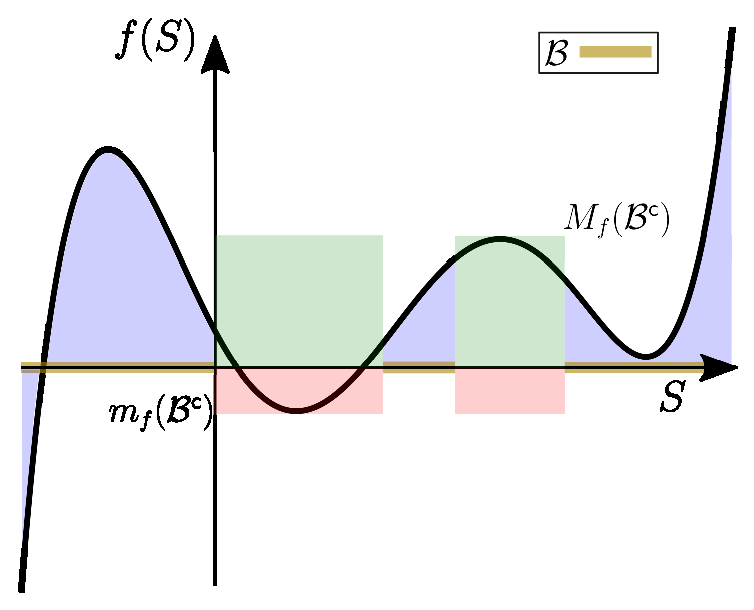
\includegraphics[width=0.4\linewidth]{bounds.eps}
	\caption{The different elements of the bounds of \cref{thm:general_bounds} are seen in the figure. The blue area is preserved as is, and is seen in the bounds as the partial expectation that we explicitly calculate ($\partialexpectation{f(\RV)}{\subSpace}$). The green and red areas are the upper ($M_f(\stcomp{\subSpace})$) and lower ($m_f(\stcomp{\subSpace})$) bounds respectively which need to be weighted by the probability that the variable is found in the compliment subset ($\measure{\stcomp{\subSpace}}$)}
	\label{fig:general_bounds}
\end{figure}
The partial expectation of a \gls{rv} may at times be easier to calculate than the total expectation (the partial expectation is related to but not equivalent to the conditional expectation). We start by introducing the following novel bounds on the difference between the expected value of a given function and its partial expectation.

\begin{theorem}
	\label{thm:general_bounds}
	Let $\RV$ be an arbitrary \gls{rv} such that $\variable\in\Space$. Consider an arbitrary function  $f\colon\Space\to\R$. Then for any subset $\subSpace\subseteq\Space$, $\lowerbound\leq\expectation{f(\RV)}{}-\partialexpectation{f(\RV)}{\subSpace}\leq\upperbound$, where:
	\begin{subequations}
	\begin{align}
		\lowerbound & = m_f(\stcomp{\subSpace})\measure{\stcomp{\subSpace}}\;,\label{eq:bound_lower}
		\\
		\upperbound & = M_f(\stcomp{\subSpace})\measure{\stcomp{\subSpace}}\;,\label{eq:bound_upper}
	\end{align}
	\end{subequations}
	and $m_f(\subSpace)$, $M_f(\subSpace)$ are defined as the infimum and supremum of $f$ over the set $\subSpace$ respectively.
\end{theorem}

\begin{proof}
	\begin{align*}
		\expectation{f(\RV)}{\RV} & = \expectation{f(\RV)\1{\RV\in \subSpace}}{\RV}+ \expectation{f(\RV)\1{\RV\in \stcomp{\subSpace}}}{\RV}
		\\
		& \leq \expectation{f(\RV)\1{\RV\in \subSpace}}{\RV} +M_f(\stcomp{\subSpace})\expectation{\1{\RV\in \stcomp{\subSpace}}}{\RV}
		\\
		& =\expectation{f(\RV)\1{\RV\in \subSpace}}{\RV} +M_f(\stcomp{\subSpace})\measure{\stcomp{\subSpace}}
		\\
		& =\partialexpectation{f(\RV)}{\subSpace} +M_f(\stcomp{\subSpace})\measure{\stcomp{\subSpace}}\qed
	\end{align*}
\end{proof}

For clarity we also provide the following definitions:
\begin{align*}
	\measure{\subSpace} & \triangleq \expectation{\1{\RV\in \subSpace}}{},\\
	\partialexpectation{f(\RV)}{\subSpace} &\equiv\expectation{f\left(\RV\right)\mid\RV\in\subSpace}{}\measure{\subSpace}.
\end{align*}

We can generalize \cref{thm:general_bounds} such the the complementary subset is split into multiple independent sets, allowing for tighter bounds.

\begin{theorem}
	\label{thm:general_bounds_multi}
	Let $\RV$ be an arbitrary \gls{rv} such that $\variable\in\Space$, and  $f\colon\Space\to\R$ be some function. Then for any subset $\subSpace\subseteq\Space$, $\lowerbound\leq\expectation{f(\RV)}{}-\partialexpectation{f(\RV)}{\subSpace}\leq\upperbound$, where:
	\begin{subequations}
		\begin{align}
			\lowerbound & = \sum_{i=1}^Nm_f(\stcompI{\subSpace}{i})\measure{\stcompI{\subSpace}{i}}\;,
			\\
			\upperbound & = \sum_{i=1}^NM_f(\stcompI{\subSpace}{i})\measure{\stcompI{\subSpace}{i}}\;,
		\end{align}
	\end{subequations}
	and $\bigcup\limits_i^N\stcompI{\subSpace}{i}=\stcomp{\subSpace}$, $\stcompI{\subSpace}{i}\cap\stcomp{\subSpace}_j=\emptyset$.
\end{theorem}
\begin{proof}
	The proof is similar to that of \cref{thm:general_bounds}, but with an extra step,
	\begin{align*}
		\expectation{f(\RV)}{\RV} & = \expectation{f(\RV)\1{\RV\in \subSpace}}{\RV}+ \expectation{f(\RV)\1{\RV\in \stcomp{\subSpace}}}{\RV}
		\\&=\expectation{f(\RV)\1{\RV\in \subSpace}}{\RV}+\sum_{i=1}^N\expectation{f(\RV)\1{\RV\in \stcompI{\subSpace}{i}}}{\RV}\\
		&\leq\partialexpectation{f(\RV)}{\subSpace} +\sum_{i=1}^NM_f(\stcompI{\subSpace}{i})\measure{\stcompI{\subSpace}{i}}\qed
	\end{align*}
\end{proof}

All proofs are given only on the upper bound when the lower bound can be reached in a similar manner. Without loss of generality $\measure{\stcomp{\subSpace}}$ and $1-\measure{\subSpace}$ will be used interchangeably depending on the need, where the use of $1-\measure{\subSpace}$ will often be preferable due to computational benefits.


\Cref{fig:general_bounds} illustrates how we change part of the function in order to bound the expectation in an adaptive fashion. To the best of our knowledge, the bounds given in \cref{thm:general_bounds} are novel and have not previously appeared in the literature.

From inequality \eqref{eq:bound_lower}, if we assume $f(\variable)\geq0$, then $\partialexpectation{f(\RV)}{\subSpace}\geq0$ and we arrive at $\expectation{f(\RV)}{}\geq m_f(\stcomp{\subSpace})\prob{\RV\in\stcomp{\subSpace}},$ which is the generalized Markov inequality~\cite{Durrett19book}. In~\cite{Ogasawara21} the authors show an improvement on the Markov inequality by also using partial expectations, although their approach assumes that the function $f(\variable)$ is non-negative strictly increasing; further generalization of the Markov inequality has also been proposed by~\cite{Bhat22spl}.


\section{Special cases}
We explore several special cases relevant to planning and computation efficiency. The following examples are but a small subset of the possible applications.

We begin with $\subSpace$ given as a superset of the subset $\subSpace^\prime$ (i.e. $\subSpace^\prime\subseteq\subSpace$), possible motivation for such an extrapolation would arise from the computation advantage in calculating the extreme values of $\stcomp{\subSpace^\prime}$ over $\stcomp{\subSpace}$. The trivial example of setting $\subSpace^\prime=\emptyset$ leads directly to the global extrema, which can be calculated offline when discussing online algorithms.
\begin{proposition}
	\label{thm:bound_diff}
	Consider a \gls{rv} $\RV$ and a function $f$ as defined in \cref{thm:general_bounds}. Let us define the subsets $\subSpace$ and $\subSpace^\prime$ such that $\subSpace^\prime\subseteq\subSpace\subseteq\Space$. Then $\lowerbound\leq\expectation{f(\RV)}{}-\partialexpectation{f(\RV)}{\subSpace}\leq\upperbound$, where:
	\begin{subequations}
		\begin{align}
			\lowerbound & = m_f(\stcomp{\subSpace^\prime})\measure{\stcomp{\subSpace}}\;,
			\\
			\upperbound & = M_f(\stcomp{\subSpace^\prime})\measure{\stcomp{\subSpace}}\;.
		\end{align}
	\end{subequations}
\end{proposition}
\begin{proof}
	From \cref{thm:general_bounds} we have
	\begin{align*}
		\expectation{f(\RV)}{\RV} & \leq\partialexpectation{f(\RV)}{\subSpace} +M_f(\stcomp{\subSpace})\measure{\stcomp{\subSpace}}
		\intertext{Given that $\subSpace^\prime\subseteq\subSpace$, then $\stcomp{\subSpace}\subseteq\stcomp{\subSpace^\prime}$\;, leading directly to $M_f(\stcomp{\subSpace})\leq M_f(\stcomp{\subSpace^\prime})$, thus}
		& \leq\partialexpectation{f(\RV)}{\subSpace} +M_f(\stcomp{\subSpace^\prime})\measure{\stcomp{\subSpace}}\qed
	\end{align*}
\end{proof}

In \cref{thm:general_bounds} the subset defines the minimum and maximum. Alternatively, one could define the subset via the minimum and maximum. (For further motivation see \cref{sec:complexity}.)

\begin{proposition}
	\label{thm:bound_epsilon}
	Consider a \gls{rv} $\RV$ and a function $f$ as defined in \cref{thm:general_bounds}. Let $\subSpace$ be a subset defined as $\subSpace\triangleq\{\variable\in\Space \mid f\left(\variable\right) < \varepsilon\lor f\left(\variable\right) > \varepsilon^\prime\}$ then $\exists\varepsilon,\varepsilon^\prime$ such that $\varepsilon\leq\varepsilon^\prime$ and $\lowerbound\leq\expectation{f(\RV)}{}-\partialexpectation{f(\RV)}{\subSpace}\leq\upperbound$, where:
	\begin{subequations}
		\begin{align}
			\lowerbound & =\varepsilon\measure{\stcomp{\subSpace}}\;,
			\\
			\upperbound & =\varepsilon^\prime\measure{\stcomp{\subSpace}}\;.
		\end{align}
	\end{subequations}
\end{proposition}
\begin{proof}
	By definition of $\subSpace$, $M_f(\stcomp{\subSpace})\leq\varepsilon^\prime$,  thus
	\begin{equation*}
		\expectation{f(\RV)}{\RV}\leq\partialexpectation{f(\RV)}{\subSpace} +\varepsilon^\prime\measure{\stcomp{\subSpace}}\qed
	\end{equation*}
\end{proof}

In the following propositions we will look into bounding the expectation of two \glspl{rv} under various assumptions. We start by simply bounding the joint expectation,

\begin{proposition}
	\label{thm:bound_multi_cond}
	Consider two arbitrary \glspl{rv} $\RV$ and $\RVI$ such that $\variable\in\Space$ and $\variableI\in\SpaceI$. Let $f\colon\left(\Space,\SpaceI\right)\to\R$ be some arbitrary function, let $\subSpaceI{\variable}$ be an arbitrary subset of $\Space$ and let $\subSpaceI{\variableI}(\variable)$ be an arbitrary subset of $\SpaceI$ as a function of $\variable$. Then $\lowerbound\leq\expectation{f(\RV,\RVI)}{\RV,\RVI}-\partialexpectation{\partialexpectation{f(\RV,\RVI)}{\subSpaceI{\variableI}(\RV)}}{\subSpaceI{\variable}}\leq\upperbound$, where:
	\begin{small}
		\begin{subequations}
			\begin{align}
				\begin{split}
					\lowerbound & = \partialexpectation{m_f(\RV,\stcompI{\subSpace}{\variableI}(\RV))\measure{\stcompI{\subSpace}{\variableI}(\RV)}}{\subSpaceI{\variable}}
					\\
					& \phantomeq+\measure{\stcompI{\subSpace}{\variable}}\left(\inf_{\variable\in\stcompI{\subSpace}{\variable}}\partialexpectation{f(\variable,\RVI)}{\subSpaceI{\variableI}(\variable)}+\inf_{\variable\in\stcompI{\subSpace}{\variable}}\left\{\measure{\stcompI{\subSpace}{\variableI}(\variable)}m_f\left(\variable,\stcompI{\subSpace}{\variableI}(\variable)\right)\right\}\right)\;,
				\end{split}
				\\
				\begin{split}
					\upperbound & = \partialexpectation{M_f(\RV,\stcompI{\subSpace}{\variableI}(\RV))\measure{\stcompI{\subSpace}{\variableI}(\RV)}}{\subSpaceI{\variable}}
					\\
					& \phantomeq+\measure{\stcompI{\subSpace}{\variable}}\left(\sup_{\variable\in\stcompI{\subSpace}{\variable}}\partialexpectation{f(\variable,\RVI)}{\subSpaceI{\variableI}(\variable)}+\sup_{\variable\in\stcompI{\subSpace}{\variable}}\left\{\measure{\stcompI{\subSpace}{\variableI}(\variable)}M_f\left(\variable,\stcompI{\subSpace}{\variableI}(\variable)\right)\right\}\right)\;,
				\end{split}
			\end{align}
		\end{subequations}
	\end{small}
	and $m_f(\subSpaceI{\variable},\RVI)\triangleq\inf\limits_{\variable\in\subSpaceI{\variable}}f(\variable,\RVI)$, $M_f(\subSpaceI{\variable},\RVI)\triangleq\sup\limits_{\variable\in\subSpaceI{\variable}}f(\variable,\RVI)$.
\end{proposition}
\begin{proof}
	We begin by applying \cref{thm:general_bounds} to the inner expectation
	\begin{align*}
		\expectation{\expectation{f(\RV,\RVI)}{\RVI\mid\RV}}{\RV} & \leq \E_{\RV}\Bigl[\partialexpectation{f(\RV,\RVI)}{\subSpaceI{\variableI}(\RV)}+M_f(\RV,\stcomp{\subSpaceI{\variableI}(\RV)})\measure{\stcomp{\subSpaceI{\variableI}(\RV)}}\Bigr]\\
		\intertext{Now applying \cref{thm:general_bounds} to the outer expectation}
		\begin{split}
			&\leq\partialexpectation{\partialexpectation{f(\RV,\RVI)}{\subSpaceI{\variableI}(\RV)}}{\subSpaceI{\variable}}
			+\partialexpectation{M_f(\RV,\stcompI{\subSpace}{\variableI}(\RV))\measure{\stcompI{\subSpace}{\variableI}(\RV)}}{\subSpaceI{\variable}}
			\\
			& \phantomeq+\measure{\stcompI{\subSpace}{\variable}}\sup_{\variable\in\stcompI{\subSpace}{\variable}}\partialexpectation{f(\variable,\RVI)}{\subSpaceI{\variableI}(\variable)}\\
			&\phantomeq
			+\measure{\stcompI{\subSpace}{\variable}}\sup_{\variable\in\stcompI{\subSpace}{\variable}}\left\{\measure{\stcompI{\subSpace}{\variableI}(\variable)}M_f\left(\variable,\stcompI{\subSpace}{\variableI}(\variable)\right)\right\}\qed
		\end{split}
	\end{align*}
\end{proof}

\begin{figure*} [h]
	\centering
	\begin{subfigure}[t]{0.45\textwidth}
		\centering
		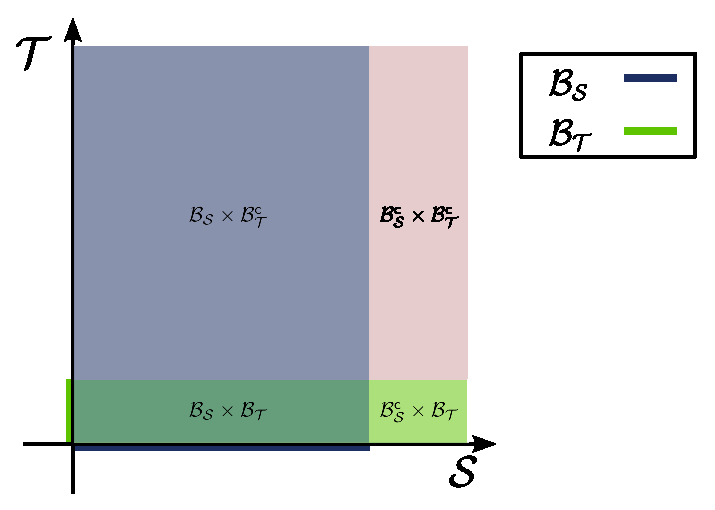
\includegraphics[width= 0.95\linewidth,clip]{independent_sets.eps}
		\caption{Visualization of the partitioning dictated by \autoref{thm:bound_multi_ind_2}. We can explicitly factor the joint domain $\subSpace$ into the Cartesian product $\subSpaceI{\variable}\times\subSpaceI{\variableI}$, thus in this scenario $\stcomp{\subSpace}=\left(\subSpaceI{\variable}\times\stcompI{\subSpace}{\variableI}\right)\cup\left(\stcompI{\subSpace}{\variable}\times\subSpaceI{\variableI}\right)\cup\left(\stcompI{\subSpace}{\variable}\times\stcompI{\subSpace}{\variableI}\right)$}
		\label{fig:ind_sets}
	\end{subfigure}
	\hfill
	\begin{subfigure}[t]{0.45\textwidth}
		\centering
		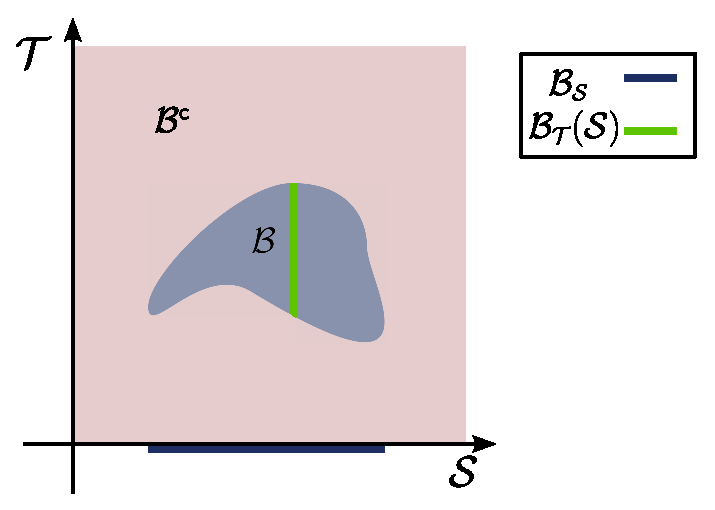
\includegraphics[width= 0.95\linewidth,clip]{dependent_sets.eps}
		\caption{Visualization of the partitioning dictated by \autoref{thm:bound_multi_cond}. The set $\subSpace$ is a general subset of the joint sample space $(\Space\times\SpaceI)$, as such it cannot necessarily be represented as a Cartesian product of two independent sets}
		\label{fig:dep_sets}
	\end{subfigure}
	\caption{Joint domain partitioning employed in the different scenarios}
	\label{fig:sets}
\end{figure*}

Let us now consider the scenario where the two variables are independent
\begin{proposition}
	\label{thm:bound_multi_ind}
	Consider two arbitrary independent \glspl{rv} $\RV$ and $\RVI$ such that $\variable\in\Space$ and $\variableI\in\SpaceI$. Let $f\colon\left(\Space,\SpaceI\right)\to\R$ be some arbitrary function and let $\subSpaceI{\variable}$ and $\subSpaceI{\variableI}$ be arbitrary subsets of $\Space$ and $\SpaceI$ respectively. Then $\lowerbound\leq\expectation{f(\RV,\RVI)}{\RV,\RVI}-\partialexpectation{\partialexpectation{f(\RV,\RVI)}{\subSpaceI{\variableI}}}{\subSpaceI{\variable}}\leq\upperbound$, where:
	\begin{subequations}
		\begin{align}
			\begin{split}
				\lowerbound & = \measure{\stcompI{\subSpace}{\variableI}}\partialexpectation{m_f(\RV,\stcompI{\subSpace}{\variableI})}{\subSpaceI{\variable}}
				+\measure{\stcompI{\subSpace}{\variable}}\inf_{\variable\in\stcompI{\subSpace}{\variable}}\partialexpectation{f(\variable,\RVI)}{\subSpaceI{\variableI}}\\
				&\phantomeq+\measure{\stcompI{\subSpace}{\variableI}}\measure{\stcompI{\subSpace}{\variable}}m_f\left(\stcompI{\subSpace}{\variable},\stcompI{\subSpace}{\variableI}\right)\;,
			\end{split}
			\\
			\begin{split}
				\upperbound & = \measure{\stcompI{\subSpace}{\variableI}}\partialexpectation{M_f(\RV,\stcompI{\subSpace}{\variableI})}{\subSpaceI{\variable}}
				+\measure{\stcompI{\subSpace}{\variable}}\sup_{\variable\in\stcompI{\subSpace}{\variable}}\partialexpectation{f(\variable,\RVI)}{\subSpaceI{\variableI}}\\
				&\phantomeq+\measure{\stcompI{\subSpace}{\variableI}}\measure{\stcompI{\subSpace}{\variable}}M_f\left(\stcompI{\subSpace}{\variable},\stcompI{\subSpace}{\variableI}\right)\;,
			\end{split}
		\end{align}
	\end{subequations}
	and $\subSpaceI{\variable}(\variableI)=\subSpaceI{\variable}$, $\subSpaceI{\variableI}(\variable)=\subSpaceI{\variableI}$.
\end{proposition}
\begin{proof}
	Given that the \glspl{rv} and subsets are independent, \autoref{thm:bound_multi_cond} simplifies trivially to the bounds
\end{proof}

We note that the relation between $\subSpaceI{\variable}$, $\subSpaceI{\variableI}$ and the joint subset ($\subSpace^\prime$) is given by $\subSpace^\prime=\subSpaceI{\variable}\times\subSpaceI{\variableI}$, this does not imply that $\stcomp{\subSpace^\prime}=\stcompI{\subSpace}{\variable}\times\stcompI{\subSpace}{\variableI}$. Furthermore it can be easily shown that the number of terms is exponential with the number of independent variables, thus a simpler bound is desirable. Under the same assumptions, but with further relaxation of the bounds, we can arrive at simplified bounds given by

\begin{proposition}
	\label{thm:bound_multi_ind_2}
	Consider two arbitrary independent \glspl{rv} $\RV$ and $\RVI$ and a function $f$ as in \autoref{thm:bound_multi_cond}. Let $\subSpaceI{\variable}$ and $\subSpaceI{\variableI}$ be arbitrary subsets of $\Space$ and $\SpaceI$ respectively. Then $\lowerbound\leq\expectation{f(\RV,\RVI)}{\RV,\RVI}-\partialexpectation{\partialexpectation{f(\RV,\RVI)}{\subSpaceI{\variableI}}}{\subSpaceI{\variable}}\leq\upperbound$, where:
	\begin{subequations}
		\begin{align}
			\lowerbound & = \left(1-\measure{\subSpaceI{\variable}}\measure{\subSpaceI{\variableI}}\right)m_f(\stcomp{\subSpace^\prime})\;, \\
			\upperbound & = \left(1-\measure{\subSpaceI{\variable}}\measure{\subSpaceI{\variableI}}\right)M_f(\stcomp{\subSpace^\prime})\;,
		\end{align}
	\end{subequations}
	and $\subSpace^\prime\triangleq\subSpaceI{\variable}\times\subSpaceI{\variableI}$.
\end{proposition}
\begin{proof}
	\begin{align*}
		\expectation{f(\RV,\RVI)}{\RV,\RVI}-\partialexpectation{\partialexpectation{f(\RV,\RVI)}{\subSpaceI{\variableI}}}{\subSpaceI{\variable}} & \leq M_f(\stcomp{\subSpace^\prime})\measure{\stcomp{\subSpace^\prime}}                                            \\
		& =M_f(\stcomp{\subSpace^\prime})\left(1-\measure{\subSpaceI{\variable}\times\subSpaceI{\variableI}}\right)         \\
		& =M_f(\stcomp{\subSpace^\prime})\left(1-\measure{\subSpaceI{\variable}}\measure{\subSpaceI{\variableI}}\right)\qed
	\end{align*}
\end{proof}

Finally, we examine how we can leverage possible knowledge of the structure of $f$ to allow for intuitive bounds on seemingly unbounded functions. We begin by bounding the $\log$ function, a common function in information theoretical rewards.

\begin{proposition}
	\label{thm:bound_log}
	Let $\RV$ and $f$ be defined as in \cref{thm:general_bounds} and consider the specific structure of $f(\variable)\triangleq g(\variable)\log h(\variable)$, where $h$ is a non-negative function and let $\subSpace$ be an arbitrary subset. Then $\lowerbound\leq\expectation{f(\RV)}{}-\partialexpectation{f(\RV)}{\subSpace}\leq\upperbound$, where:
	\begin{subequations}
		\begin{align}
			\lowerbound & = \measure{\stcomp{\subSpace}}
			\min\left\{m_g(\stcomp{\subSpace})\log m_h(\stcomp{\subSpace}),M_g(\stcomp{\subSpace})\log m_h(\stcomp{\subSpace})\right\}\;,\label{eq:bound_lower_log}\\
			\upperbound & = \measure{\stcomp{\subSpace}}
			\max\left\{m_g(\stcomp{\subSpace})\log M_h(\stcomp{\subSpace}),M_g(\stcomp{\subSpace})\log M_h(\stcomp{\subSpace})\right\}\;\label{eq:bound_upper_log}.
		\end{align}
	\end{subequations}
\end{proposition}
\begin{proof}
	Assuming $g(\variable)\geq 0$
	\begin{equation*}
		M_f(\stcomp{\subSpace})=\max_{\variable\in\stcomp{\subSpace}}\{g(\variable)\log h(\variable)\}\leq\max\left\{
		\begin{aligned}
			& M_g(\stcomp{\subSpace})\log M_h(\stcomp{\subSpace})\;, \\
			& m_g(\stcomp{\subSpace})\log M_h(\stcomp{\subSpace})
		\end{aligned}\right\}\qed
	\end{equation*}
	The assumption of $g(\variable)\geq 0$ can also be easily dropped for a more general bound.
\end{proof}

We continue to formulate the case of joint expectation on the $\log$ function.
\begin{proposition}
	\label{thm:bound_exp}
	Let $\RV\in\R^N$ and $\RVI\in\R^m$ be two \gls{rv}. Let $f$ be of the specific structure $f(\variable)\triangleq \expectation{\log g(\variable,\RVI)}{\RVI\mid\variable}\colon\R^N\to\R$, where $g$ is non-negative. Thus by \cref{thm:general_bounds} the difference $\expectation{\expectation{\log g(\RV,\RVI)}{\RVI\mid\RV}}{\RV}-
	\partialexpectation{\expectation{\log g(\RV,\RVI)}{\RVI\mid\RV}}{\subSpace}$ is bounded above and below by
	\begin{align}
			\lowerbound=&\measure{\stcomp{\subSpace}}\log\left(\inf_{\variable\in\stcomp{\subSpace},\variableI}g(\variable,\variableI)\right)\;,\label{eq:bound_lower_exp}\\
			\upperbound=&\measure{\stcomp{\subSpace}}\log\left(\sup_{\variable\in\stcomp{\subSpace},\variableI}g(\variable,\variableI)\right)\;.\label{eq:bound_upper_exp}
	\end{align}
\end{proposition}
\begin{proof}
	\begin{align*}
		\expectation{\expectation{\log f(\RV,\RVI)}{\RVI\mid\RV}}{\RV}&=\expectation{\expectation{\log \frac{f(\RV,\RVI)}{\varepsilon(\RVI)}}{\RVI\mid\RV}}{\RV}+\expectation{\expectation{\log \varepsilon(\RVI)}{\RVI\mid\RV}}{\RV}
		\\
		&=\expectation{\expectation{\log \frac{f(\RV,\RVI)}{\varepsilon(\RVI)}}{\RVI\mid\RV}}{\RV}+\expectation{\log \varepsilon(\RVI)}{\RVI}
		\\
		\begin{split}
			&\leq\partialexpectation{\expectation{\log f(\RV,\RVI)}{\RVI\mid\RV}}{\subSpace}-\partialexpectation{\expectation{\log \varepsilon(\RVI)}{\RVI\mid\RV}}{\subSpace}\\
			&\phantomeq+\left(1-\measure{\subSpace}\right)\log\max_{\variableI}\varepsilon(\variableI)+\expectation{\log \varepsilon(\RVI)}{\RVI}\qed
		\end{split}
	\end{align*}
\end{proof}

\section{Bound Properties}\label{sec:properties}
The bounds from \cref{thm:general_bounds} have several desirable properties for bound based decision making algorithms, the principle of which is incrementality, allowing for the tightening of the bounds while reusing parts of the original bounds.


\begin{corollary}[Incrementality]
	\label{thm:incrementality}
	Given a subset $\subSpace^\prime$ such that $\subSpace\subseteq\subSpace^\prime$ the bounds as defined in \cref{thm:general_bounds} can be calculated incrementally for $\subSpace^\prime$.  In other words, calculations only within the new subset $\subSpace_{\textrm{\textup{new}}}\triangleq\subSpace^\prime\setminus\subSpace$ are needed. This can be expressed explicitly as follows:
	\begin{align}
		\partialexpectation{f(\RV)}{\subSpace^\prime} & =\partialexpectation{f(\RV)}{\subSpace}+\partialexpectation{f(\RV)}{\subSpace_{\textrm{\textup{new}}}}\;,
		\\
		\measure{\subSpace^\prime}& =\measure{\subSpace}+\measure{\subSpace_{\textrm{\textup{new}}}}\;.
	\end{align}
	The infimum and supremum are partially incremental, depending on the scenario as described below
	\begin{subequations}
		\begin{align}
			m_f(\stcomp{\subSpace^\prime})
			& =\begin{cases}
				m_f(\stcomp{\subSpace}) & \textup{if}\ m_f(\stcomp{\subSpace})<m_f(\subSpace_{\textrm{\textup{new}}}) \\
				\textup{by definition}  & \textup{else}
			\end{cases}\;, \\
			M_f(\stcomp{\subSpace^\prime})
			& =\begin{cases}
				M_f(\stcomp{\subSpace}) & \textup{if}\ M_f(\stcomp{\subSpace})>M_f(\subSpace_{\textrm{\textup{new}}}) \\
				\textup{by definition}  & \textup{else}
			\end{cases}\;.
		\end{align}
	\end{subequations}
\end{corollary}
\begin{proof}
	\begin{align*}
		\partialexpectation{f(\RV)}{\subSpace^\prime} & =\expectation{f(\RV)\1{\RV\in\subSpace^\prime}}{}\\
		& =\expectation{f(\RV)\left(\1{\RV\in\subSpace}+\1{\RV\in\subSpace_{\textrm{\textup{new}}}}\right)}{}\\
		& =\partialexpectation{f(\RV)}{\subSpace}+\partialexpectation{f(\RV)}{\subSpace_{\textrm{\textup{new}}}}
	\end{align*}
	The proof for $\measure{\subSpace^\prime}$ follows the same logic.

	$\stcomp{\subSpace}=\subSpace_{\textrm{\textup{new}}}\cup\stcomp{\subSpace^\prime}$, thus $M_f(\stcomp{\subSpace})=\max\{M_f(\subSpace_{\textrm{\textup{new}}}),M_f(\stcomp{\subSpace^\prime})\}$, if $M_f(\stcomp{\subSpace})>M_f(\subSpace_{\textrm{\textup{new}}})$, then implicitly $M_f(\stcomp{\subSpace})\neq M_f(\subSpace_{\textrm{\textup{new}}})$ leaving us with $M_f(\stcomp{\subSpace})=M_f(\stcomp{\subSpace^\prime})$. If $M_f(\stcomp{\subSpace})=M_f(\subSpace_{\textrm{\textup{new}}})$ then we gain no information on $M_f(\stcomp{\subSpace^\prime})$, leaving us with $M_f(\stcomp{\subSpace})\geq M_f(\stcomp{\subSpace^\prime})$.
\end{proof}


\begin{corollary}[Convergence]
	\label{thm:convergence}
	The bounds as defined in \cref{thm:general_bounds} converge to zero with respect to the set $\subSpace$, meaning the partial expectation converges to the true expectation when $\subSpace=\Space$.
\end{corollary}
\begin{proof}
	By definition $\measure{\Space}=1$ and $\partialexpectation{f(\RV)}{\Space}=\expectation{f(\RV)}{\RV}$, thus we immediately arrive at $\lowerbound(\Space)=\upperbound(\Space)=0$
\end{proof}

\begin{corollary}[Monotonicity]
	\label{thm:monotonicity}
	The bounds as defined in \cref{thm:general_bounds} are monotonic with respect to the subspace. Specifically:
	\begin{subequations}
		\begin{align}
			\lowerbound(\subSpace) & \leq\lowerbound(\subSpace^\prime)\;, \\
			\upperbound(\subSpace) & \geq\upperbound(\subSpace^\prime)\;,
		\end{align}
	\end{subequations}
	for $\subSpace\subseteq\subSpace^\prime$. Moreover these bounds are strictly monotonic when $\subSpace_{\textrm{\textup{new}}}$ is measurable (i.e. $\measure{\subSpace_{\textrm{\textup{new}}}}\neq0$).
\end{corollary}
\begin{proof}
	Let us define $\subSpace^\prime\supseteq\subSpace$, thus $M_f(\stcomp{\subSpace^\prime})\leq M_f(\stcomp{\subSpace})$, by \autoref{thm:incrementality} we find that $\measure{\subSpace}\leq\measure{\subSpace^\prime}$ thus
	\begin{equation*}
		M_f(\stcomp{\subSpace^\prime})\left(1-\measure{\subSpace^\prime}\right) \leq M_f(\stcomp{\subSpace})\left(1-\measure{\subSpace}\right)\qed
	\end{equation*}
\end{proof}

\section{Complexity}\label{sec:complexity}
Let us denote the complexity of a single evaluation of the function $f$ by $O(\abs{f})$, and the complexity of finding bounds on the infimum and supremum of $f$ by $O(\abs{m})$ and $O(\abs{M})$ respectively. Then the complexity of calculating the bounds in \cref{thm:general_bounds} is given by the complexity of the partial expectation over the set $\subSpace$ and the complexity of finding the infimum and supremum over the set $\stcomp{\subSpace}$, $O\left(\abs{f}\cdot\abs{\subSpace}+\left(\abs{m}+\abs{M}\right)\cdot\abs{\stcomp{\subSpace}}\right)$. When $O(\abs{m}+\abs{M})\ll O(\abs{f})$ then computational savings of approximately $O(\abs{f}\cdot\abs{\stcomp{\subSpace}})$ are attained.

The above assumes that the complexity of division into subsets is trivial. But alternatively, one could select subsets defined by their infimum and supremum as in \autoref{thm:bound_epsilon}, thus $O(\abs{m})=O(\abs{M})=O(1)$, but the complexity is simply transferred into finding which elements belong in each subset, this is the case with the Markov inequality. The choice between these two scenarios is per use case.

\section{Estimators and Novel Probabilistic Bounds}
An estimator $\hat{P}(\states{})$ of the distribution $\prob{\states{}}$ is given by: $\sum\limits_{i=1}^{N}w^i\delta\left(\states{}-\states{}^i\right)$, where $(\weight{}{i},\states{}^i)$ is a weighted particle sampled from $\prob{\states{}}$. Thus by defining $\estimator{\cdot}{\statesRV{}\sim \prob{\states{}}} \triangleq \expectation{\cdot}{\statesRV{}\sim \hat{P}(\states{})}$, we find $\estimator{g(\states{})}{\statesRV{}}=\int\sum_{i=1}^{N}\weight{}{i}\delta\left(\states{}-\states{}^i\right)g(\states{})\D\states{}=\sum_{i=1}^{N}\weight{}{i}g(\states{}^i),$
which is in practice the expectation with respect to a discrete variable with $\hat{P}\left(\states{}^i\right)=\weight{}{i}$. Thus \cref{thm:general_bounds}, with no additional changes, is also valid for estimators, where the sample space is defined by the set of samples. This also holds true for functions of the pdf, both of the form $\estimator{f(\hat{P}(\states{}))}{}$ and $\estimator{f(\prob{\states{}})}{}$ with appropriate attention given to constructing the bound itself.

When the pdf itself is also estimated as in the case of $\hat{P}(\states{})$, then bounds on the estimated weights may be useful for \cref{thm:general_bounds}, thus we provide \autoref{thm:estimator_bound}.

\begin{corollary}
	\label{thm:estimator_bound}
	Let $\{(\weight{}{i},\variable^i)\}^N_{i=1}$ be a set of normalized particles sampled from the distribution $\prob{\variable}$. Then the weights ($\weight{}{i}$) are bounded below and above by
	\begin{subequations}
		\begin{align}
			\lowerbound & =1-\frac{\max \prob{\variable}}{\frac{\min \prob{\variable}}{N-1}+\max\prob{\variable}}\;, \\
			\upperbound & =1-\frac{\min \prob{\variable}}{\frac{\max \prob{\variable}}{N-1}+\min\prob{\variable}}\;.
		\end{align}
	\end{subequations}
\end{corollary}
\begin{proof}
	\begin{align*}
		\min_i \weight{}{i} & =\min_i \frac{\prob{\variable^i}}{\sum_{i=1}^N\prob{\variable^i}}
		\intertext{Let us denote, without loss of generality, $\min\limits_i \prob{\variable^i}$ as $\prob{\variable^1}$, thus}
		& =\frac{\prob{\variable^1}}{\prob{\variable^1}+\sum_{i=2}^N\prob{\variable^i}}          \\
		& \geq\frac{\prob{\variable^1}}{\prob{\variable^1}+(N-1)\max\limits_i\prob{\variable^i}} \\
		& \geq\frac{\min\prob{\variable}}{\min\prob{\variable}+(N-1)\max\prob{\variable}}\qed
	\end{align*}
\end{proof}

The use of estimators in the field of robotics is often present when we use Monte-Carlo methods for reasoning about future actions. As we are working with estimators, we are interested in how close the estimator is to the theoretical expectation. Via Hoeffding's inequality we arrive at two main claims of our paper; the first is a probabilistic bound between the true expectation and the estimated partial expectation.

\begin{theorem}
	\label{thm:partial_hoeffding}
	Consider the set of samples $\{\variable^i\}_{i=1}^N$ drawn from $\RV$, then
	\begin{align*}
		\prob{\lowerbound\leq\expectation{f(\RV)}{}-\partialestimator{f(\RV)}{\subSpace_n}\leq\upperbound}\geq1-\delta&&\forall\delta\in(0,1)\;,
	\end{align*}
	where $\subSpace_n\triangleq\{\variable^i\}_{i=1}^n$ for $n\leq N$,
	\begin{subequations}
		\begin{align}
			\lowerbound & =-\sqrt{\frac{\Delta_f^2}{2N}\log\frac{2}{\delta}}+m_f(\stcomp{\subSpace_n})\estimatedmeasure{\stcomp{\subSpace_n}}\;, \\
			\upperbound & =\sqrt{\frac{\Delta_f^2}{2N}\log\frac{2}{\delta}}+M_f(\stcomp{\subSpace_n})\estimatedmeasure{\stcomp{\subSpace_n}}\;,
		\end{align}
	\end{subequations}
	and $\Delta_f(\subSpace)\triangleq M_f(\subSpace)-m_f(\subSpace)$
\end{theorem}
\begin{proof}
	From Hoeffding's inequality on the \gls{rv} $f(\RV)$ the following holds
	\begin{equation*}
		\prob{\abs{\expectation{f(\RV)}{}-\estimator{f(\RV)}{}}\leq t}\geq1-\delta,
	\end{equation*}
	where $t=\sqrt{\frac{\Delta_f^2}{2N}\log\frac{2}{\delta}}$. From the absolute value we have two inequalities, we fill focus on the upper bound.
	With the addition of inequality \refeq{eq:bound_upper} for some subset $\subSpace_n$ of the samples
	\begin{align*}
		& \expectation{f(\RV)}{}-\estimator{f(\RV)}{}+\estimator{f(\RV)}{}-\partialestimator{f(\RV)}{\subSpace}\leq t+M_f(\stcomp{\subSpace})\estimatedmeasure{\stcomp{\subSpace}}, \\
		& \expectation{f(\RV)}{}-\partialestimator{f(\RV)}{\subSpace}\leq t+M_f(\stcomp{\subSpace})\estimatedmeasure{\stcomp{\subSpace}}.
	\end{align*}
	Repeating the procedure for the lower bounds results in the complete bounds.
\end{proof}

It can be shown that when comparing \cref{thm:partial_hoeffding} to the case of simply taking a Hoeffding bound with $n$ samples from the original distribution, our bounds are tighter when the following inequality is satisfied:
\begin{equation}
	C\cdot\left(\sqrt{\frac{1}{n}}-\sqrt{\frac{1}{N}}\right)\geq\Delta_f(\stcomp{\subSpace_n})\estimatedmeasure{\stcomp{\subSpace_n}}\;,
\end{equation}
where $C\triangleq \Delta_f\sqrt{2\log\frac{2}{\delta}}$. The bound is relevant when $N$ samples are drawn, but evaluation of the function $f$ for all $N$ samples is undesirable, allowing for a controlled way to remove some samples.

The second of the claims is a probabilistic bound between the true expectation and the estimated conditional expectation.
\begin{theorem}
	\label{thm:conditional_hoeffding}
	Let $\RV$ be some \gls{rv} and let $\subSpace\subseteq\Space$ be some sample space. Consider the set of samples $\{\variable^i\}_{i=1}^N$ drawn from $\RV\1{\RV\in\subSpace}$, then
	\begin{align*}
		\prob{\lowerbound\leq\expectation{f(\RV)}{}-\measure{\subSpace}\condestimator{f(\RV)}{\subSpace}{}\leq\upperbound}\geq1-\delta&&\forall\delta\in(0,1)\;,
	\end{align*}
	where
	\begin{subequations}
		\begin{align}
			\lowerbound & =-\measure{\subSpace}\sqrt{\frac{\Delta_f(\subSpace)^2}{2N}\log\frac{2}{\delta}}+m_f(\stcomp{\subSpace})\measure{\stcomp{\subSpace}}\;, \\
			\upperbound & =\measure{\subSpace}\sqrt{\frac{\Delta_f(\subSpace)^2}{2N}\log\frac{2}{\delta}}+M_f(\stcomp{\subSpace})\measure{\stcomp{\subSpace}}\;.
		\end{align}
	\end{subequations}
\end{theorem}
\begin{proof}
	From Hoeffding's inequality on the \gls{rv} $f(\RV)$ the following holds
	\begin{equation*}
		\prob{\abs{\condexpectation{f(\RV)}{\subSpace}{}-\condestimator{f(\RV)}{\subSpace}{}}\leq t}\geq1-\delta\;,
	\end{equation*}
	where $t=\sqrt{\frac{\Delta_f^2}{2N}\log\frac{2}{\delta}}$. From the absolute value we have two inequalities, we fill focus on the upper bound.
	Multiplying though by $\measure{\subSpace}$ and the addition of inequality \refeq{eq:bound_upper} we find
	\begin{align*}
		& \partialexpectation{f(\RV)}{\subSpace}-\measure{\subSpace}\condestimator{f(\RV)}{\subSpace}{}\leq \measure{\subSpace}t\;,\\
		\begin{split}
			& \expectation{f(\RV)}{}-\partialexpectation{f(\RV)}{\subSpace}+\partialexpectation{f(\RV)}{\subSpace}-\measure{\subSpace}\condestimator{f(\RV)}{\subSpace}{} \\
			& \leq \measure{\subSpace}t+M_f(\stcomp{\subSpace})\measure{\stcomp{\subSpace}}\;,
		\end{split} \\
		& \expectation{f(\RV)}{}-\measure{\subSpace}\condestimator{f(\RV)}{\subSpace}{}\leq\measure{\subSpace}t+M_f(\stcomp{\subSpace})\measure{\stcomp{\subSpace}}\;.
	\end{align*}
\end{proof}

\noindent Similarly to \cref{thm:partial_hoeffding}, \cref{thm:conditional_hoeffding} offers tighter bounds in comparison to the vanilla Hoeffding bound under the following inequality constraint:
\begin{equation}
	C\cdot\left(\Delta_f-\measure{\subSpace}\Delta_f(\subSpace)\right)\geq \measure{\stcomp{\subSpace}}\Delta_f(\stcomp{\subSpace})\;,
\end{equation}
where $C\triangleq\sqrt{\frac{2}{N}\log\frac{2}{\delta}}$.

Utilizing this bound is relevant when one would like to focus the sampling procedure on a specific area of the distribution, or if only a proposal distribution is available on part of the support, while still being able to make a claim on the expectation. It may be desirable to apply another Hoeffding inequality in order to estimate and bound with the use of $\estimatedmeasure{\subSpace}$.

%We can bound the expectation of $f(\RV)$ by sampling via importance sampling only from the subspace $\subSpace$ via some proposal distribution $q(\variable)$, where the sample space $\subSpace$ is such that $\int_\subSpace q(\variable)\D\variable=1$. This extension of the standard Hoeffding inequality incorporates the use of \cref{thm:general_bounds}, allowing for concentration inequality on the expected value with respect to a partial estimator, and not the complete estimator as is traditionally done.
%
%We will address one special case where $q(\variable)\triangleq \frac{p(\variable)\1{\variable\in\subSpace}}{\int_\subSpace p(\variable)\D\variable}=\frac{p(\variable)\1{\variable\in\subSpace}}{\measure{\subSpace}}$. Under these conditions
%\begin{equation}
%	\partialexpectation{f(\RV)}{\subSpace}\equiv\measure{\subSpace}\expectation{f\left(\RV\right)}{\RV\sim q},
%\end{equation}
%and the bounds of \cref{thm:partial_hoeffding} still hold with probability $\left((1-\delta)(1-\delta^\prime)\right)^2$ for the difference $\expectation{f(\RV)}{\RV\sim p}-
%\measure{\subSpace}\estimator{f\left(\RV\right)}{\RV\sim q}$. Although it might prove necessary to estimate $\measure{\subSpace}$ and apply an additional use of the Hoeffding's inequality.
\chapter{Planning}

The bounds discussed in \cref{sec:bounds} have applications in various contexts, both for \glspl{pomdp} and other domains. In this section, we examine how these bounds can be effectively employed in \gls{bsp}. We start with general formulations of bounds for \glspl{pomdp}. Subsequently, we focus on information-theoretic rewards, particularly entropy. Finally, we address the challenges of planning in high-dimensional state spaces.

\section{Reward and Value Functions}

In the context of planning, the general reward function is denoted as $\reward{\blf{},\pi,\blf{}^\prime}$. Our goal in planning is to bound the cumulative expected reward, as represented in \eqref{eq:value_function}, where the expectation is explicitly given on observations and implicitly for states in the reward structure. By reducing the domain over which this expectation is calculated ---whether with respect to states, observations, or both--- we can achieve improved computational efficiency (see \cref{sec:complexity}) while providing formal performance guarantees. In this paper we focus on bounding the expectation with respect to the observations, although similar bounds can be formulated for the state space.

We begin by bounding the expected reward with respect to the observation space:
\begin{equation}
		\expectation{\reward{\blf{},\pi}}{\observationsRV{}}-\partialexpectation{\reward{\blf{},\pi(\blf{})}}{\subSpaceI{\observations{}}}
		\leq\measure{\stcompI{\subSpace}{\observations{}}}\sup_{\observations{}\in\stcompI{\subSpace}{\observations{}}}\reward{\blf{},\pi(\blf{})}\;,
\end{equation}
where $\subSpaceI{\observations{}}\subseteq\observationSpace$.

In many planning scenarios, the belief dependent reward is assumed to have a structure of $\reward{\blf{},\pi(\blf{})}\equiv \expectation{R(\blf{}(\statesRV{}),\statesRV{},\pi(\blf{}))}{\statesRV{}\sim\blf{}}$. For such cases, we can derive bounds on the reward with respect to the state space:
\begin{equation}
		\expectation{R(\blf{}(\statesRV{}),\statesRV{},\pi(\blf{}))}{\statesRV{}\sim\blf{}}-\partialexpectation{R(\blf{}(\statesRV{}),\statesRV{},\pi(\blf{}))}{\subSpaceI{\states{}}}
		\leq\measure{\stcompI{\subSpace}{\states{}}}\sup_{\states{}\in\stcompI{\subSpace}{\states{}}}R(\blf{}(\states{}),\states{},\pi(\blf{}))\;,
\end{equation}
where $\subSpaceI{\states{}}\subseteq\stateSpace$.

Not all rewards depend on the belief. State-dependent rewards, given by $\expectation{R(\statesRV{},\pi(\blf{}))}{\statesRV{}\sim\blf{}}$, follow a similar pattern but often benefit from known $R_{\min}$ and $R_{\max}$ values, simplifying the bounds to:
\begin{equation}
	\begin{split}
		\expectation{R(\statesRV{},\pi(\blf{}))}{\statesRV{}\sim\blf{}}-\partialexpectation{R(\statesRV{},\pi(\blf{}))}{\subSpaceI{\states{}}}&\leq\measure{\stcompI{\subSpace}{\states{}}}\sup_{\states{}\in\stcompI{\subSpace}{\states{}}}R(\states{},\pi(\blf{}))             \\
		 &\leq\measure{\stcompI{\subSpace}{\states{}}}R_{\max}\;.
	\end{split}
\end{equation}
If we further look at action sequences and not policies, then the case of state dependent rewards further simplifies matters by being independent of the observations.

These bounds can be jointly used to reduce the computational complexity by reducing the state and observation spaces concurrently.

With these reward bounds, we can proceed to bound the value function. When bounding with respect to the state space:
\begin{corollary}
	\label{thm:val_func_bounds_states}
	$\lowerbound^\pi(\blf{k})\leq V^\pi(\blf{k})-\bar{V}^\pi(\blf{k})\leq\upperbound^\pi(\blf{k})$, where:
	\begin{subequations}
		\begin{align}
			\lowerbound\nolimits^\pi(\blf{k})& =\measure{\stcompI{\subSpace}{k}}\inf_{\states{k}\in\stcompI{\subSpace}{k}}R_k+\sum_{l=k+1}^{k+L}\gamma^{l-k}\expectation{\measure{\stcompI{\subSpace}{l}}\inf_{\states{l}\in\stcompI{\subSpace}{l}}\boldsymbol{R}_l}{\observationsRV{k+1:l}}\;,\\
			\upperbound\nolimits^\pi(\blf{k}) & =\measure{\stcompI{\subSpace}{k}}\sup_{\states{k}\in\stcompI{\subSpace}{k}}R_k+\sum_{l=k+1}^{k+L}\gamma^{l-k}\expectation{\measure{\stcompI{\subSpace}{l}}\sup_{\states{l}\in\stcompI{\subSpace}{l}}\boldsymbol{R}_l}{\observationsRV{k+1:l}}\;,\\
			\bar{V}^\pi(\blf{k}) & =\partialexpectation{\boldsymbol{R}_k}{\subSpaceI{k}}+\sum_{l=k+1}^{k+L}\gamma^{l-k}\expectation{\partialexpectation{\boldsymbol{R}_l}{\subSpaceI{l}}}{\observationsRV{k+1:l}}\;.
		\end{align}
	\end{subequations}
	and $R_k\triangleq R(\blf{k}(\states{k}),\states{k},\pi(\blf{k}))$.
\end{corollary}
\begin{proof}
	Applying \cref{thm:general_bounds} to $\expectation{\boldsymbol{R}_l}{\states{l}}$ and summing for the cumulative reward results in the desired bounds.
\end{proof}
\noindent We use the shorthand $R_k\triangleq R(\blf{k}(\states{k}),\states{k},\pi(\blf{k}))$.

Expressing the bounds in a recursive manner, as is done for the value function with the Bellman equation \eqref{eq:bellman}, we find the following:
\begin{corollary}
	\label{thm:val_func_bounds_states_bellman}
	$\lowerbound^\pi(\blf{t})\leq V^\pi(\blf{t})-\bar{V}^\pi(\blf{t})\leq\upperbound^\pi(\blf{t})\quad\forall t\in[k,k+L]$, where:
	\begin{subequations}
		\begin{align}
			\lowerbound\nolimits^\pi(\blf{t}) & =\measure{\stcompI{\subSpace}{t}}\inf_{\states{t}\in\stcompI{\subSpace}{t}}R_t+\gamma\expectation{\lowerbound(\blf{t+1})}{\observationsRV{t+1}}\;,\\
			\upperbound\nolimits^\pi(\blf{t}) & =\measure{\stcompI{\subSpace}{t}}\sup_{\states{t}\in\stcompI{\subSpace}{t}}R_t+\gamma\expectation{\upperbound(\blf{t+1})}{\observationsRV{t+1}}\;,\\
			\bar{V}^\pi(\blf{t}) & =\partialexpectation{\boldsymbol{R}_t}{\subSpaceI{t}}
			+\gamma\expectation{\bar{V}^\pi(\blf{t+1})}{\observationsRV{t+1}}\;.
		\end{align}
	\end{subequations}
	and $\lowerbound^\pi(\blf{k+L})=\upperbound^\pi(\blf{k+L})=V^\pi(\blf{k+L})=\bar{V}^\pi(\blf{k+L})=0$, $\subSpaceI{t}\subseteq\stateSpace$.
\end{corollary}
\begin{proof}
	Proof by induction:

	\textbf{\underline{base case:}}
	\begin{align*}
		\upperbound\nolimits^\pi(\blf{k+L-1})&=\measure{\stcompI{\subSpace}{k+L-1}}\sup_{\states{k+L-1}\in\stcompI{\subSpace}{k+L-1}}R_t+\gamma\expectation{\upperbound(\blf{k+L})}{\observationsRV{k+L}}\\
		&=\measure{\stcompI{\subSpace}{k+L-1}}\sup_{\states{k+L-1}\in\stcompI{\subSpace}{k+L-1}}R_t\;,\\
		\bar{V}^\pi(\blf{k+L-1}) & =\partialexpectation{\boldsymbol{R}_t}{\subSpaceI{k+L-1}}
		+\gamma\expectation{\bar{V}^\pi(\blf{k+L})}{\observationsRV{k+L}}\\
		&=\partialexpectation{\boldsymbol{R}_{k+L-1}}{\subSpaceI{k+L-1}}\;,\\
		V^\pi(\blf{k+L-1})&=\expectation{\boldsymbol{R}_{k+L-1}}{\statesRV{k+L-1}}
		+\gamma\expectation{V^\pi(\blf{k+L})}{\observationsRV{k+L}}\\
		&=\expectation{\boldsymbol{R}_{k+L-1}}{\statesRV{k+L-1}}\;.
	\end{align*}
	Put together we find that the inequality holds as it is a direct consequence of \cref{thm:general_bounds} for $\expectation{\boldsymbol{R}_{k+L-1}}{\statesRV{k+L-1}}$.

	\textbf{\underline{induction step:}}
	Let us assume that $V^\pi(\blf{t+1})-\bar{V}^\pi(\blf{t+1})\leq\upperbound(\blf{t+1})$ then
	\begin{align*}
		V^\pi(\blf{t})&-\bar{V}^\pi(\blf{t})\\
		\begin{split}
			&=\expectation{R(\blf{t}(\statesRV{t}),\statesRV{t},\pi(\blf{t}))}{\statesRV{t}}-\partialexpectation{R(\blf{t}(\statesRV{t}),\statesRV{t},\pi(\blf{t}))}{\subSpaceI{t}} \\
			&\phantomeq+\gamma\left(\expectation{V^\pi(\blf{t+1})-\bar{V}^\pi(\blf{t+1})}{\observationsRV{t+1}}\right)
		\end{split}    \\
		\begin{split}
			&\leq\expectation{R(\blf{t}(\statesRV{t}),\statesRV{t},\pi(\blf{t}))}{\statesRV{t}}-\partialexpectation{R(\blf{t}(\statesRV{t}),\statesRV{t},\pi(\blf{t}))}{\subSpaceI{t}} \\
			&\phantomeq+\gamma\left(\expectation{\upperbound(\blf{t+1})}{\observationsRV{t+1}}\right)
		\end{split} \\
		&\leq\measure{\subSpaceI{t+1}}\sup_{\stcompI{\subSpace}{t+1}}R(\blf{t}(\statesRV{t}),\statesRV{t},\pi(\blf{t}))+\gamma\left(\expectation{\upperbound(\blf{t+1})}{\observationsRV{t+1}}\right)\qed
	\end{align*}
\end{proof}

As was done for the reward, we can also bound with respect to the observation space:
\begin{corollary}
	\label{thm:val_func_bounds_obs}
	$\lowerbound^\pi(\blf{k})\leq V^\pi(\blf{k})-\bar{V}^\pi(\blf{k})\leq\upperbound^\pi(\blf{k})$, where:
	\begin{small}
		\begin{subequations}
			\begin{align}
				\lowerbound\nolimits^\pi(\blf{k})& =\sum_{l=k}^{k+L-1}\gamma^{l-k}\measure{\stcompI{\subSpace}{k+1:l+1}\mid\blf{k},\pi}\inf_{\observations{k+1:l+1}\in\stcompI{\subSpace}{k+1:l+1}}\reward{\blf{l},\pi_l,\blf{l+1}}\;, \\
				\upperbound\nolimits^\pi(\blf{k})& =\sum_{l=k}^{k+L-1}\gamma^{l-k}\measure{\stcompI{\subSpace}{k+1:l+1}\mid\blf{k},\pi}\sup_{\observations{k+1:l+1}\in\stcompI{\subSpace}{k+1:l+1}}\reward{\blf{l},\pi_l,\blf{l+1}}\;, \\
				\bar{V}^\pi(\blf{k}) & =\sum_{l=k}^{k+L-1}\gamma^{l-k}\partialexpectation{\reward{\blf{l},\pi_l,\blf{l+1}}}{\subSpaceI{k+1:l+1}\mid\blf{k},\pi}\;,
			\end{align}
		\end{subequations}
	\end{small}
	and $\subSpaceI{k+1:l+1}\subseteq\observationSpace^{l-k}$ which is the joint observation space over time.
\end{corollary}
\begin{proof}
	Beginning with \eqref{eq:value_function} we look for bounds on $\expectation{\reward{\blf{l},\pi_l,\blf{l+1}}}{\observationsRV{k+1:l+1}\mid\blf{k},\pi}$. Applying \cref{thm:general_bounds} leads us directly to the bounds for a single time step. Subsequently we sum over all time-steps.
\end{proof}

If we wish to propagate the choice of subset not just to the immediate expected reward, but through to the entire value function, thus completely eliminating specific realizations of observations from the objective function, we find:
\begin{corollary}
	\label{thm:val_func_bounds_obs_bellman}
	$\lowerbound^\pi(\blf{t})\leq V^\pi(\blf{t})-\bar{V}^\pi(\blf{t})\leq\upperbound^\pi(\blf{t})\quad\forall t\in[k,k+L]$, where:
	\begin{small}
		\begin{subequations}
			\begin{align}
				\begin{split}
					\lowerbound\nolimits^\pi(\blf{t})&=\measure{\stcompI{\subSpace}{t+1}\mid\blf{t},\pi}\Bigl(\inf_{\stcompI{\subSpace}{t+1}}\reward{\blf{t},\pi_t,\blf{t+1}}+\gamma\inf_{\stcompI{\subSpace}{t+1}}\bar{V}^\pi(\blf{t+1})\Bigr)\\
					&+
					\gamma\Bigl(\measure{\stcompI{\subSpace}{t+1}\mid\blf{t},\pi}\inf_{\stcompI{\subSpace}{t+1}}\lowerbound(\blf{t+1})+\partialexpectation{\lowerbound(\blf{t+1})}{\subSpaceI{t+1}\mid\blf{t},\pi}\Bigr)\;,
				\end{split}\\
				\begin{split}
					\upperbound\nolimits^\pi(\blf{t})&=\measure{\stcompI{\subSpace}{t+1}\mid\blf{t},\pi}\Bigl(\sup_{\stcompI{\subSpace}{t+1}}\reward{\blf{t},\pi_t,\blf{t+1}}+\gamma\sup_{\stcompI{\subSpace}{t+1}}\bar{V}^\pi(\blf{t+1})\Bigr)\\
					&+
					\gamma\Bigl(\measure{\stcompI{\subSpace}{t+1}\mid\blf{t},\pi}\sup_{\stcompI{\subSpace}{t+1}}\lowerbound(\blf{t+1})+\partialexpectation{\lowerbound(\blf{t+1})}{\subSpaceI{t+1}\mid\blf{t},\pi}\Bigr)\;,
				\end{split}\\
				\bar{V}^\pi(\blf{t}) &=\partialexpectation{\reward{\blf{t},\pi_t,\blf{t+1}}}{\subSpaceI{t+1}\mid\blf{t},\pi}+\gamma\partialexpectation{\bar{V}^\pi(\blf{t+1})}{\subSpaceI{t+1}\mid\blf{t},\pi}\;,
			\end{align}
		\end{subequations}
	\end{small}
	and $\lowerbound^\pi(\blf{k+L})=\upperbound^\pi(\blf{k+L})=V^\pi(\blf{k+L})=\bar{V}^\pi(\blf{k+L})=0$ and $\subSpaceI{t}\subseteq\observationSpace$.
\end{corollary}
\begin{proof}
	Proof by induction:

	\textbf{\underline{base case:}}
	\begin{align*}
		\upperbound\nolimits^\pi(\blf{k+L-1})&=\measure{\stcompI{\subSpace}{k+L}\mid\blf{k+L-1},\pi}\Bigl(\sup_{\stcompI{\subSpace}{k+L}}\reward{\blf{k+L-1},\pi_t,\blf{k+L}}+\gamma\sup_{\stcompI{\subSpace}{k+L}}\bar{V}^\pi(\blf{k+L})\Bigr)\\
		&+
		\gamma\Bigl(\measure{\stcompI{\subSpace}{k+L}\mid\blf{t},\pi}\sup_{\stcompI{\subSpace}{k+L}}\lowerbound(\blf{k+L})+\partialexpectation{\lowerbound(\blf{k+L})}{\subSpaceI{k+L}\mid\blf{k+L-1},\pi}\Bigr)\\
		&=\measure{\stcompI{\subSpace}{k+L}\mid\blf{k+L-1},\pi}\Bigl(\sup_{\stcompI{\subSpace}{k+L}}\reward{\blf{k+L-1},\pi_t,\blf{k+L}}\Bigr)\;,\\
		\bar{V}^\pi(\blf{k+L-1}) &=\partialexpectation{\reward{\blf{k+L-1},\pi_{k+L-1},\blf{k+L}}}{\subSpaceI{k+L}\mid\blf{k+L-1},\pi}+\gamma\partialexpectation{\bar{V}^\pi(\blf{k+L})}{\subSpaceI{k+L}\mid\blf{k+L-1},\pi}\\
		&=\partialexpectation{\reward{\blf{k+L-1},\pi_{k+L-1},\blf{k+L}}}{\subSpaceI{k+L}\mid\blf{k+L-1},\pi}\;,\\
		V^\pi(\blf{k+L-1})&=\expectation{\reward{\blf{k+L-1},\pi_{k+L-1},\blf{k+L}}}{\observationsRV{k+L}\mid\blf{k+L-1},\pi}+\gamma\expectation{V^\pi(\blf{k+L})}{\observationsRV{k+L}}\\
		&=\expectation{\reward{\blf{k+L-1},\pi_{k+L-1},\blf{k+L}}}{\observationsRV{k+L}\mid\blf{k+L-1},\pi}\;.
	\end{align*}
	Put together we find that the inequality holds as it is a direct consequence of \cref{thm:general_bounds} for $\expectation{\reward{\blf{k+L-1},\pi_{k+L-1},\blf{k+L}}}{\observationsRV{k+L}\mid\blf{k+L-1},\pi}$.

	\textbf{\underline{induction step:}}
	, let us assume that $V^\pi(\blf{t+1})-\bar{V}^\pi(\blf{t+1})\leq\upperbound(\blf{t+1})$ then
	\begin{align*}
		V^\pi(\blf{t})&-\bar{V}^\pi(\blf{t})\\
		\begin{split}
			=&\expectation{\reward{\blf{t},\pi_t,\blf{t+1}}}{\observationsRV{t+1}}-\partialexpectation{\reward{\blf{t},\pi_t,\blf{t+1}}}{\subSpaceI{t+1}}\\
			&+\gamma\left(\expectation{V^\pi(\blf{t+1})}{\observationsRV{t+1}}-\partialexpectation{\bar{V}^\pi(\blf{t+1})}{\subSpaceI{t+1}}\right)
		\end{split}\\
		\begin{split}
			\leq&\measure{\stcompI{\subSpace}{t+1}}\sup_{\stcompI{\subSpace}{t+1}}\reward{\blf{t},\pi_t,\blf{t+1}}\\
			&+\partialexpectation{\reward{\blf{t},\pi_t,\blf{t+1}}}{\subSpaceI{t+1}}-\partialexpectation{\reward{\blf{t},\pi_t,\blf{t+1}}}{\subSpaceI{t+1}}\\
			&+\gamma\measure{\stcompI{\subSpace}{t+1}}\sup_{\stcompI{\subSpace}{t+1}}V^\pi(\blf{t+1})+\gamma\left(\partialexpectation{V^\pi(\blf{t+1})}{\subSpaceI{t+1}}-\partialexpectation{\bar{V}^\pi(\blf{t+1})}{\subSpaceI{t+1}}\right)
		\end{split}\\
		\begin{split}
			\leq&\measure{\stcompI{\subSpace}{t+1}}\sup_{\stcompI{\subSpace}{t+1}}\reward{\blf{t},\pi_t,\blf{t+1}}\\
			&+\gamma\left(\measure{\stcompI{\subSpace}{t+1}}\sup_{\stcompI{\subSpace}{t+1}}V^\pi(\blf{t+1})+\partialexpectation{\upperbound(\blf{t+1})}{\subSpaceI{t+1}}\right)
		\end{split}\\
		\begin{split}
			=&\measure{\stcompI{\subSpace}{t+1}}\sup_{\stcompI{\subSpace}{t+1}}\reward{\blf{t},\pi_t,\blf{t+1}}\\
			&+\gamma\measure{\stcompI{\subSpace}{t+1}}\sup_{\stcompI{\subSpace}{t+1}}\left(V^\pi(\blf{t+1})-\bar{V}^\pi(\blf{t+1})+\bar{V}^\pi(\blf{t+1})\right) \\
			&+\gamma\partialexpectation{\upperbound(\blf{t+1})}{\subSpaceI{t+1}}
		\end{split}\\
		\begin{split}
			\leq&\measure{\stcompI{\subSpace}{t+1}}\sup_{\stcompI{\subSpace}{t+1}}\reward{\blf{t},\pi_t,\blf{t+1}}\\
			&+\gamma\measure{\stcompI{\subSpace}{t+1}}\sup_{\stcompI{\subSpace}{t+1}}\left(\upperbound(\blf{t+1})+\bar{V}^\pi(\blf{t+1})\right)+\gamma\partialexpectation{\upperbound(\blf{t+1})}{\subSpaceI{t+1}}
		\end{split}\\
		\begin{split}
			\leq&\measure{\stcompI{\subSpace}{t+1}}\sup_{\stcompI{\subSpace}{t+1}}\reward{\blf{t},\pi_t,\blf{t+1}}\\
			&+\gamma\measure{\stcompI{\subSpace}{t+1}}\left(\sup_{\stcompI{\subSpace}{t+1}}\upperbound(\blf{t+1})+\sup_{\stcompI{\subSpace}{t+1}}\bar{V}^\pi(\blf{t+1})\right)+\gamma\partialexpectation{\upperbound(\blf{t+1})}{\subSpaceI{t+1}}\qed
		\end{split}
	\end{align*}
\end{proof}

In \autoref{thm:val_func_bounds_obs_bellman} the choice of subsets $\subSpaceI{t}$ is used for bounding the expected reward as well as the cumulative expected rewards. If one were to construct a belief tree, then the choice of subset would be analogous to pruning the branches indicated by $\stcomp{\subSpace}$.

An alternative approach which proves to be more manageable to formulate is to take the partial expectation only with respect to the immediate expected reward. This approach still allows for closed-loop planning, but does not prune the tree, instead it simplifies calculations for the immediate expected reward.
\begin{corollary}
	\label{thm:val_func_immediate_bounds_obs_bellman}
	$\lowerbound(\blf{t})\leq V^\pi(\blf{t})-\bar{V}^\pi(\blf{t})\leq\upperbound(\blf{t})\quad\forall t\in[k,k+L]$, where:
	\begin{small}
		\begin{subequations}
			\begin{align}
				\lowerbound(\blf{t}) & =\measure{\stcompI{\subSpace}{t+1}}\inf_{\stcompI{\subSpace}{t+1}}\reward{\blf{t},\pi_t,\blf{t+1}}+\gamma\expectation{\lowerbound(\blf{t+1})}{\observationsRV{t+1}}\;,\\
				\upperbound(\blf{t}) & =\measure{\stcompI{\subSpace}{t+1}}\sup_{\stcompI{\subSpace}{t+1}}\reward{\blf{t},\pi_t,\blf{t+1}}+\gamma\expectation{\upperbound(\blf{t+1})}{\observationsRV{t+1}}\;,\\
				\bar{V}^\pi(\blf{t}) & =\partialexpectation{\reward{\blf{t},\pi_{t},\blf{t+1}}}{\subSpaceI{t+1}}+\gamma\expectation{\bar{V}^\pi(\blf{t+1})}{\observationsRV{t+1}}\;.
			\end{align}
		\end{subequations}
	\end{small}
	and $\lowerbound^\pi(\blf{k+L})=\upperbound^\pi(\blf{k+L})=V^\pi(\blf{k+L})=\bar{V}^\pi(\blf{k+L})=0$ and $\subSpaceI{t}\subseteq\observationSpace$.
\end{corollary}
\begin{proof}
	Proof by induction:

	\textbf{\underline{base case:}}
	\begin{align*}
		\upperbound\nolimits^\pi(\blf{k+L-1})&=\measure{\stcompI{\subSpace}{k+L}}\sup_{\stcompI{\subSpace}{k+L}}\reward{\blf{k+L-1},\pi_{k+L-1},\blf{k+L}}+\gamma\expectation{\upperbound(\blf{k+L})}{\observationsRV{k+L}}\\
		&=\measure{\stcompI{\subSpace}{k+L}}\sup_{\stcompI{\subSpace}{k+L}}\reward{\blf{k+L-1},\pi_{k+L-1},\blf{k+L}}\;,\\
		\bar{V}^\pi(\blf{k+L-1})&=\partialexpectation{\reward{\blf{k+L-1},\pi_{k+L-1},\blf{k+L}}}{\subSpaceI{k+L}}+\gamma\expectation{\bar{V}^\pi(\blf{k+L})}{\observationsRV{k+L}}\\
		&=\partialexpectation{\reward{\blf{k+L-1},\pi_{k+L-1},\blf{k+L}}}{\subSpaceI{k+L}}\;,\\
		V^\pi(\blf{k+L-1})&=\expectation{\reward{\blf{k+L-1},\pi_{k+L-1},\blf{k+L}}}{\observationsRV{k+L}\mid\blf{k+L-1},\pi}+\gamma\expectation{V^\pi(\blf{k+L})}{\observationsRV{k+L}}\\
		&=\expectation{\reward{\blf{k+L-1},\pi_{k+L-1},\blf{k+L}}}{\observationsRV{k+L}\mid\blf{k+L-1},\pi}\;.
	\end{align*}
	Put together we find that the inequality holds as it is a direct consequence of \cref{thm:general_bounds} for $\expectation{\reward{\blf{k+L-1},\pi_{k+L-1},\blf{k+L}}}{\observationsRV{k+L}\mid\blf{k+L-1},\pi}$.

	\textbf{\underline{induction step:}}
	Let us assume that $V^\pi(\blf{t+1})-\bar{V}^\pi(\blf{t+1})\leq\upperbound(\blf{t+1})$ then
	\begin{align*}
		V^\pi(\blf{t})-&\bar{V}^\pi(\blf{t})\\
		\begin{split}
			&=\expectation{\reward{\blf{t},\pi_t,\blf{t+1}}}{\observationsRV{t+1}}-\partialexpectation{\reward{\blf{t},\pi_t,\blf{t+1}}}{\subSpaceI{t+1}}\\
			&\phantomeq+\gamma\Bigl(\expectation{V^\pi(\blf{t+1})}{\observationsRV{t+1}}-\expectation{\bar{V}^\pi(\blf{t+1})}{\observationsRV{t+1}}\Bigr)
		\end{split}\\
		\begin{split}
			&\leq\measure{\stcompI{\subSpace}{t+1}}\sup_{\stcompI{\subSpace}{t+1}}\reward{\blf{t},\pi_t,\blf{t+1}}\\
			&\phantomeq+\partialexpectation{\reward{\blf{t},\pi_t,\blf{t+1}}}{\subSpaceI{t+1}}-\partialexpectation{\reward{\blf{t},\pi_t,\blf{t+1}}}{\subSpaceI{t+1}}\\
			&\phantomeq+\gamma\expectation{V^\pi(\blf{t+1})-\bar{V}^\pi(\blf{t+1})}{\observationsRV{t+1}}
		\end{split}\\
		&\leq\measure{\stcompI{\subSpace}{t+1}}\sup_{\stcompI{\subSpace}{t+1}}\reward{\blf{t},\pi_t,\blf{t+1}}+\gamma\expectation{\upperbound(\blf{t+1})}{\observationsRV{t+1}}\qed
	\end{align*}
\end{proof}

For a specific planning scenario, assuming that the desired bounds are now available, we refer to previous works~\cite{Sztyglic22iros,Barenboim22ijcai} to explore the applications of planning with bounds.


\section{Conditional Entropy Bounds}\label{sec:cond_ent_bounds}
We will be looking exclusively at two subsequent planning steps, thus we will drop the use of time indices, using $\square\equiv\square_k$ and $\square^\prime\equiv\square_{k+1}$.
In the case where our reward is entropy, we can expand the conditional entropy as follows via Bayes rule
\begin{equation}
		\expectation{\condEntropy{\statesRV{}}{\observationsRV{}}}{\observationsRV{}}\equiv\condEntropy{\statesRV{}}{\observationsRV{}}=\entropy{\statesRV{}}+\condEntropy{\observationsRV{}}{\statesRV{}}-\entropy{\observationsRV{}}.\label{eq:bayes_entropy}
\end{equation}
To demonstrate the functionality of these approaches we look to realize the bounds with information theoretical rewards. We look to \autoref{thm:val_func_immediate_bounds_obs_bellman} as our value function bounds, which requires bounds on the expected reward. For the choice of entropy ($\entropy{\statesRV{}}$) as the reward, our expected reward becomes conditional entropy ($\condEntropy{\statesRV{}}{\observationsRV{}}$). We prove novel bounds on the conditional entropy with respect to the observation space that utilize \cref{thm:general_bounds}.

\begin{theorem}
	\label{thm:entropy_bounds}
	The conditional entropy of the \gls{rv} $\statesRV{}$ given the \gls{rv} $\observationsRV{}$ can be bounded by the difference of the partial expectation with respect to $\observationsRV{}$. Thus $\lowerbound\leq\condEntropy{\statesRV{}}{\observationsRV{}}-\simplecondEntropy{\statesRV{}}{\observationsRV{}}{\observations{}}\leq\upperbound$, where:
	\begin{small}
		\begin{subequations}
			\begin{align}
				\lowerbound&=-\measure{\stcomp{\subSpace}}\Bigl(\log\sup_{\observations{}\in\stcomp{\subSpace}}M_{\observations{}}-\log m_{\norm{\observations{}}}(\stcomp{\subSpace})\Bigr)-\upperbound_\subSpace\Bigl(\expectation{\log C_{pq}}{\observationsRV{}}\Bigr)\;,
				\\
				\upperbound& =-\measure{\stcomp{\subSpace}}\Bigl(\log\inf_{\observations{}\in\stcomp{\subSpace}}m_{\observations{}}-\log M_{\norm{\observations{}}}(\stcomp{\subSpace})\Bigr)\;,\\
				\begin{split}
					\simplecondEntropy{\statesRV{}}{\observationsRV{}}{\observations{}}&\triangleq\entropy{\statesRV{}}+\log\pnorm{\prob{\states{}}}{q}{\states{}}\\
					&\phantomeq-\partialexpectation{\expectation{\log\probcond{\observationsRV{}}{\statesRV{}}}{\statesRV{}\sim\probcond{\statesRV{}}{\observationsRV{}}}+\log\pnorm{\probcond{\observationsRV{}}{\states{}}}{p}{\states{}}}{\subSpace}\;.
				\end{split}
			\end{align}
		\end{subequations}
	\end{small}
	The definition of $\upperbound_\subSpace\Bigl(\expectation{\log C_{pq}}{\observationsRV{}}\Bigr)$ can be seen in the proof.
	\begin{align*}
		m_{\norm{\observations{}}}(\subSpace) &\triangleq\inf_{\observations{}\in\subSpace}\pnorm{\probcond{\observations{}}{\states{}}}{p}{\states{}}\;,&M_{\norm{\observations{}}}(\subSpace) &\triangleq\sup_{\observations{}\in\subSpace}\pnorm{\probcond{\observations{}}{\states{}}}{p}{\states{}}\;,\\
		m_{\observations{}}&\triangleq\inf_{\states{}}\probcond{\observations{}}{\states{}}\;,&M_{\observations{}}&\triangleq\sup_{\states{}}\probcond{\observations{}}{\states{}}\;.
	\end{align*}
\end{theorem}
\begin{proof}
	We begin by applying Bayes theorem to $\condEntropy{\statesRV{}}{\observationsRV{}}$
	\begin{equation}
		\expectation{\condEntropy{\statesRV{}}{\observationsRV{}}}{\observationsRV{}}\equiv\condEntropy{\statesRV{}}{\observationsRV{}}=\entropy{\statesRV{}}+\condEntropy{\observationsRV{}}{\statesRV{}}-\entropy{\observationsRV{}}\;.
	\end{equation}
	The term $\entropy{\statesRV{}}$ is independent of $\observationsRV{}$ and so remains unchanged. The next two terms we bound via \autoref{thm:observation_bounds} and \autoref{thm:normalizer_bounds} from \cref{sec:appendix} which are subsequently shown and proven. Collecting the bounds on all the terms results directly in the bounds mentioned in the theorem.
	\begin{equation*}
		\begin{split}
			\upperbound_\subSpace\left(\expectation{\log C_{pq}}{\observationsRV{}}\right)&=-\frac{\log p}{p}-\frac{\log q}{q}-\partialexpectation{\log m_{\observations{}}}{\subSpace}-\log m_{\states{}}\\
			&\phantomeq+ \partialexpectation{\log\left(m_{\states{}}M_{\states{}}^{q-1}+m_{\observations{}}M_{\observations{}}^{p-1}\right)}{\subSpace}\\
			&\phantomeq+\measure{\stcomp{\subSpace}}\log\Biggl( m_{\states{}}M_{\states{}}^{q-1}+\inf_{\observations{}\in\stcomp{\subSpace}}m_{\observations{}}\Biggl(\sup_{\observations{}\in\stcomp{\subSpace}}M_{\observations{}}\Biggr)^{p-1}\Biggr) \\
			&\phantomeq-\measure{\stcomp{\subSpace}}\log\inf_{\observations{}\in\stcomp{\subSpace}}m_{\observations{}}\;,
		\end{split}
	\end{equation*}
	where $M_{\states{}}\triangleq\sup\prob{\states{}}$ and $m_{\states{}}\triangleq\inf\prob{\states{}}$.
\end{proof}
We use $\pnorm{\cdot}{p}{\variable}$ to represent the p\tsups{th}-norm with respect to the integration variable $\variable$. We mention that $m_{\norm{\observations{}}}(\subSpace)\geq \inf\limits_{\observations{}\in\subSpace}m_{\observations{}}$ and $M_{\norm{\observations{}}}(\subSpace)\leq \sup\limits_{\observations{}\in\subSpace}M_{\observations{}}$ and can be used to loosen the bounds if needed.

To the best of our knowledge the conditional entropy bounds introduced above are novel. Similar works that provide simplification with guarantees for information theoretical rewards are \cite{Sztyglic22iros,Barenboim22ijcai,Yotam24tro}. We leave comparative studies to these works for future research.

Subsequent to Bayesian factorization of the conditional entropy ($\condEntropy{\statesRV{}}{\observationsRV{}}=\entropy{\statesRV{}}+\condEntropy{\observationsRV{}}{\statesRV{}}-\entropy{\observationsRV{}}$) in \cref{thm:entropy_bounds}, $\entropy{\statesRV{}}$ assumes that the actions are independent of the observations. In the non-myopic case this implies an open-loop setting, as would be necessitated in the context of \autoref{thm:val_func_bounds_obs}. As \autoref{thm:val_func_immediate_bounds_obs_bellman} is myopic in the partial expectation, its application in \cref{thm:entropy_bounds} still allows for closed-loop planning.

\section{Entropy Estimator}
A common estimator of the entropy is the Boers estimator \cite{Boers10fusion}. We will look into bounding this estimator with respect to reducing the state space. The Boers estimator is given by:
\begin{equation}
	\label{eq:boers}
		\entropyEstimator{\statesRV{}^\prime}=\log\left(\sum_{i=1}^N\weight{}{i}\probcond{\observations{}^\prime}{\states{}^{\prime i}}\right)-\sum_{i=1}^N\weight{}{\prime i}\log\left(\probcond{\observations{}^\prime }{\states{}^{\prime i}}\sum_{j=1}^N\weight{}{j}\probcond{\states{}^{\prime i}}{\states{}^{j}}\right)
\end{equation}
Where $\{\states{}^i,\weight{}{i}\}_{i=1}^N$ are samples from belief $\blf{}$ and are self normalized.

In order to bound the estimator we begin by expressing it in terms of expectations, allowing for the straight forwards application of our bounds.
\begin{equation}
		\entropyEstimator{\statesRV{}^\prime}=\log\estimator{\probcond{\observations{}^\prime}{\statesRV{}^\prime}}{\statesRV{}}-\estimator{\log\probcond{\observations{}^\prime}{\statesRV{}^\prime}}{\statesRV{}^\prime}-\estimator{\log\estimator{\probcond{\statesRV{}^\prime}{\statesRV{}}}{\statesRV{}}}{\statesRV{}^\prime}
\end{equation}
We can now apply the bounds from \cref{thm:general_bounds}.
\begin{lemma}
	\label{thm:boers_bounds}
	$\lowerbound\leq\entropyEstimator{\statesRV{}^\prime}-\simplentropy{\statesRV{}^\prime}{}\leq\upperbound$, where:
	\begin{small}
	\begin{subequations}
		\begin{align}
			\begin{split}
				\lowerbound &=\log\left(\sum\limits_{i=1}^n\weight{}{i}\probcond{\observations{}^\prime}{\states{}^{\prime i}}+\left(1-\sum\limits_{i=1}^n\weight{}{i}\right)\inf\limits_{j\in[n+1,N]}\probcond{\observations{}^\prime}{\states{}^{\prime j}}\right) \\
				& \phantomeq-\left(1-\sum_{i=1}^n\weight{}{\prime i}\right)\log\sup_{j\in[n+1,N]}\probcond{\observations{}^\prime}{\states{}^{\prime j}}\\
				&\phantomeq-\sum_{i=1}^n\weight{}{\prime i}\log\left(\sum_{j=1}^n\weight{}{j}\probcond{\states{}^{\prime i}}{\states{}^j}+\left(1-\sum\limits_{j=1}^n\weight{}{j}\right)\sup_{j\in[n+1,N]}\probcond{\states{}^{\prime i}}{\states{}^j}\right)\\
				& \phantomeq-\left(1-\sum_{i=1}^n\weight{}{\prime i}\right)\log\left(\sup_{i\in[n+1,N]}\sum_{j=1}^n\weight{}{j}\probcond{\states{}^{\prime i}}{\states{}^j}+\left(1-\sum\limits_{j=1}^n\weight{}{j}\right)\sup_{i,j\in[n+1,N]}\probcond{\states{}^{\prime i}}{\states{}^j}\right)
			\end{split} \\
			\begin{split}
				\upperbound & =\log\left(\sum\limits_{i=1}^n\weight{}{i}\probcond{\observations{}^\prime}{\states{}^{\prime i}}+\left(1-\sum\limits_{i=1}^n\weight{}{i}\right)\sup\limits_{j\in[n+1,N]}\probcond{\observations{}^\prime}{\states{}^{\prime j}}\right) \\
				& \phantomeq-\left(1-\sum_{i=1}^n\weight{}{\prime i}\right)\log\inf_{j\in[n+1,N]}\probcond{\observations{}^\prime}{\states{}^{\prime j}}\\
				&\phantomeq-\sum_{i=1}^n\weight{}{\prime i}\log\left(\sum_{j=1}^n\weight{}{j}\probcond{\states{}^{\prime i}}{\states{}^j}+\left(1-\sum\limits_{j=1}^n\weight{}{j}\right)\inf_{j\in[n+1,N]}\probcond{\states{}^{\prime i}}{\states{}^j}\right)\\
				& \phantomeq-\left(1-\sum_{i=1}^n\weight{}{\prime i}\right)\log\left(\inf_{i\in[n+1,N]}\sum_{j=1}^n\weight{}{j}\probcond{\states{}^{\prime i}}{\states{}^j}+\left(1-\sum\limits_{j=1}^n\weight{}{j}\right)\inf_{i,j\in[n+1,N]}\probcond{\states{}^{\prime i}}{\states{}^j}\right)
			\end{split}\\
			\simplentropy{\statesRV{}^\prime}{} & \triangleq-\sum_{i=1}^n\weight{}{\prime i}\log\probcond{\observations{}^\prime}{\states{}^{\prime i}}
		\end{align}
	\end{subequations}
	\end{small}
\end{lemma}
\begin{proof}
	\begin{align}
		\begin{split}
			\entropyEstimator{\statesRV{}^\prime}&=\log\estimator{\probcond{\observations{}^\prime}{\statesRV{}^\prime}}{\statesRV{}}-\estimator{\log\probcond{\observations{}^\prime}{\statesRV{}^\prime}}{\statesRV{}^\prime}\\
			&\phantomeq-\estimator{\log\estimator{\probcond{\statesRV{}^\prime}{\statesRV{}}}{\statesRV{}}}{\statesRV{}^\prime}
		\end{split}\\
		\begin{split}
			&\leq\log\left(\partialestimator{\probcond{\observations{}^\prime}{\statesRV{}^\prime}}{\subSpace}+\estimatedmeasure{\stcomp{\subSpace}}\sup_{\stcomp{\subSpace}}\probcond{\observations{}^\prime}{\states{}^\prime}\right)\\
			&\phantomeq-\partialestimator{\log\probcond{\observations{}^\prime}{\statesRV{}^\prime}}{\subSpace^\prime}-\estimatedmeasure{\stcomp{\subSpace^\prime}}\inf_{\stcomp{\subSpace^\prime}}\log\probcond{\observations{}^\prime}{\states{}^\prime}\\
			&\phantomeq-\estimator{\log\left(\partialestimator{\probcond{\statesRV{}^\prime}{\statesRV{}}}{\subSpace}+\estimatedmeasure{\stcomp{\subSpace}}\inf_{\stcomp{\subSpace}}\probcond{\statesRV{}^\prime}{\states{}}\right)}{\statesRV{}^\prime}
		\end{split}\\
		\begin{split}
			&\leq\log\left(\partialestimator{\probcond{\observations{}^\prime}{\statesRV{}^\prime}}{\subSpace}+\estimatedmeasure{\stcomp{\subSpace}}\sup_{\stcomp{\subSpace}}\probcond{\observations{}^\prime}{\states{}^\prime}\right)\\
			&\phantomeq-\partialestimator{\log\probcond{\observations{}^\prime}{\statesRV{}^\prime}}{\subSpace^\prime}-\estimatedmeasure{\stcomp{\subSpace^\prime}}\inf_{\stcomp{\subSpace^\prime}}\log\probcond{\observations{}^\prime}{\states{}^\prime}\\
			&\phantomeq-\partialestimator{\log\left(\partialestimator{\probcond{\statesRV{}^\prime}{\statesRV{}}}{\subSpace}+\estimatedmeasure{\stcomp{\subSpace}}\inf_{\stcomp{\subSpace}}\probcond{\statesRV{}^\prime}{\states{}}\right)}{\subSpace^\prime}\\
			&\phantomeq-\estimatedmeasure{\stcomp{\subSpace^\prime}}\inf_{\stcomp{\subSpace^\prime}}\log\left(\partialestimator{\probcond{\states{}^\prime}{\statesRV{}}}{\subSpace}+\estimatedmeasure{\stcomp{\subSpace}}\inf_{\stcomp{\subSpace}}\probcond{\states{}^\prime}{\states{}}\right)
		\end{split}\\
		\begin{split}
			&\leq\log\left(\partialestimator{\probcond{\observations{}^\prime}{\statesRV{}^\prime}}{\subSpace}+\estimatedmeasure{\stcomp{\subSpace}}\sup_{\stcomp{\subSpace}}\probcond{\observations{}^\prime}{\states{}^\prime}\right)\\
			&\phantomeq-\partialestimator{\log\probcond{\observations{}^\prime}{\statesRV{}^\prime}}{\subSpace^\prime}-\estimatedmeasure{\stcomp{\subSpace^\prime}}\log\inf_{\stcomp{\subSpace^\prime}}\probcond{\observations{}^\prime}{\states{}^\prime}\\
			&\phantomeq-\partialestimator{\log\left(\partialestimator{\probcond{\statesRV{}^\prime}{\statesRV{}}}{\subSpace}+\estimatedmeasure{\stcomp{\subSpace}}\inf_{\stcomp{\subSpace}}\probcond{\statesRV{}^\prime}{\states{}}\right)}{\subSpace^\prime}\\
			&\phantomeq-\estimatedmeasure{\stcomp{\subSpace^\prime}}\log\left(\inf_{\stcomp{\subSpace^\prime}}\partialestimator{\probcond{\states{}^\prime}{\statesRV{}}}{\subSpace}+\estimatedmeasure{\stcomp{\subSpace}}\inf_{\stcomp{\subSpace},\stcomp{\subSpace^\prime}}\probcond{\states{}^\prime}{\states{}}\right)
		\end{split}
	\end{align}
\end{proof}

The computational complexity of the bounds, assuming that the supremum and infimum are $O(1)$, is now $O(n^2)$ as seen in the definition of $\simplentropy{\statesRV{}^\prime}{}$ from the double summation, in contrast to the previous complexity of $O(N^2)$, assuming that $\abs{\subSpaceI{k+1}}=\abs{\subSpaceI{k}}=n$. In \cite{Sztyglic22iros} bounds on the Boer's estimator are also derived, but with a complexity of $O(nN)$. Let us further simplify \cref{thm:boers_bounds} by utilizing the global extrema, thus

\begin{proposition}
	\label{thm:boers_bounds_simple}
	$\lowerbound\leq\entropyEstimator{\statesRV{}^\prime}-\simplentropy{\statesRV{}^\prime}{}\leq\upperbound$, where:
	\begin{subequations}
		\begin{align}
			\begin{split}
				\lowerbound & =\log\left(\sum\limits_{i=1}^n\weight{}{i}\probcond{\observations{}^\prime}{\states{}^{\prime i}}+\left(1-\sum\limits_{i=1}^n\weight{}{i}\right)m_{\observations{}^\prime}\right) \\
				&\phantomeq-\sum_{i=1}^n\weight{}{\prime i}\log\left(\sum_{j=1}^n\weight{}{j}\probcond{\states{}^{\prime i}}{\states{}^j}+\left(1-\sum\limits_{i=1}^n\weight{}{i}\right)M_{\states{}}\right)\\
				& \phantomeq-\left(1-\sum_{i=1}^n\weight{}{\prime i}\right)\left(\log M_{\states{}}+\log M_{\observations{}^\prime}\right)
			\end{split}\\
			\begin{split}
				\upperbound & =\log\left(\sum\limits_{i=1}^n\weight{}{i}\probcond{\observations{}^\prime}{\states{}^{\prime i}}+\left(1-\sum\limits_{i=1}^n\weight{}{i}\right)M_{\observations{}^\prime}\right) \\
				&\phantomeq-\sum_{i=1}^n\weight{}{\prime i}\log\left(\sum_{j=1}^n\weight{}{j}\probcond{\states{}^{\prime i}}{\states{}^j}+\left(1-\sum\limits_{i=1}^n\weight{}{i}\right)m_{\states{}}\right)\\
				& \phantomeq-\left(1-\sum_{i=1}^n\weight{}{\prime i}\right)\left(\log m_{\states{}}+\log m_{\observations{}^\prime}\right)
			\end{split}\\
			\simplentropy{\statesRV{}^\prime}{} & \triangleq-\sum_{i=1}^n\weight{}{\prime i}\log\probcond{\observations{}^\prime}{\states{}^{\prime i}}
		\end{align}
	\end{subequations}
	and we define $m_{\states{}}\triangleq\inf\limits_{\states{},\states{}^\prime}\probcond{\states{}^\prime}{\states{}}$, $M_{\states{}}\triangleq\sup\limits_{\states{},\states{}^\prime}\probcond{\states{}^\prime}{\states{}}$, $m_{\observations{}}\triangleq\inf\limits_{\states{}}\probcond{\observations{}}{\states{}}$, and $M_{\observations{}}\triangleq\sup\limits_{\states{}}\probcond{\observations{}}{\states{}}$.
\end{proposition}
\begin{proof}
	\begin{align}
		\begin{split}
			&\leq\log\left(\partialestimator{\probcond{\observations{}^\prime}{\statesRV{}^\prime}}{\subSpace}+\estimatedmeasure{\stcomp{\subSpace}}\sup_{\stcomp{\subSpace}}\probcond{\observations{}^\prime}{\states{}^\prime}\right)\\
			&\phantomeq-\partialestimator{\log\probcond{\observations{}^\prime}{\statesRV{}^\prime}}{\subSpace^\prime}-\estimatedmeasure{\stcomp{\subSpace^\prime}}\log\inf_{\stcomp{\subSpace^\prime}}\probcond{\observations{}^\prime}{\states{}^\prime}\\
			&\phantomeq-\partialestimator{\log\left(\partialestimator{\probcond{\statesRV{}^\prime}{\statesRV{}}}{\subSpace}+\estimatedmeasure{\stcomp{\subSpace}}\inf_{\stcomp{\subSpace}}\probcond{\statesRV{}^\prime}{\states{}}\right)}{\subSpace^\prime}\\
			&\phantomeq-\estimatedmeasure{\stcomp{\subSpace^\prime}}\log\left(\inf_{\stcomp{\subSpace^\prime}}\partialestimator{\probcond{\states{}^\prime}{\statesRV{}}}{\subSpace}+\estimatedmeasure{\stcomp{\subSpace}}\inf_{\stcomp{\subSpace},\stcomp{\subSpace^\prime}}\probcond{\states{}^\prime}{\states{}}\right)
		\end{split}\\
		\begin{split}
			&\leq\log\left(\partialestimator{\probcond{\observations{}^\prime}{\statesRV{}^\prime}}{\subSpace}+\estimatedmeasure{\stcomp{\subSpace}}M_{\observations{}^\prime}\right)\\
			&\phantomeq-\partialestimator{\log\probcond{\observations{}^\prime}{\statesRV{}^\prime}}{\subSpace^\prime}-\estimatedmeasure{\stcomp{\subSpace^\prime}}\log m_{\observations{}^\prime}\\
			&\phantomeq-\partialestimator{\log\left(\partialestimator{\probcond{\statesRV{}^\prime}{\statesRV{}}}{\subSpace}+\estimatedmeasure{\stcomp{\subSpace}}m_{\states{}}\right)}{\subSpace^\prime}\\
			&\phantomeq-\estimatedmeasure{\stcomp{\subSpace^\prime}}\log m_{\states{}}
		\end{split}\\
		\begin{split}
			&=\log\left(\partialestimator{\probcond{\observations{}^\prime}{\statesRV{}^\prime}}{\subSpace}+\estimatedmeasure{\stcomp{\subSpace}}M_{\observations{}^\prime}\right)\\
			&\phantomeq-\partialestimator{\log\probcond{\observations{}^\prime}{\statesRV{}^\prime}}{\subSpace^\prime}\\
			&\phantomeq-\partialestimator{\log\left(\partialestimator{\probcond{\statesRV{}^\prime}{\statesRV{}}}{\subSpace}+\estimatedmeasure{\stcomp{\subSpace}}m_{\states{}}\right)}{\subSpace^\prime}\\
			&\phantomeq-\estimatedmeasure{\stcomp{\subSpace^\prime}}\left(\log m_{\states{}}+\log m_{\observations{}^\prime}\right)
		\end{split}
	\end{align}
\end{proof}

\section{High Dimensional Aspect}\label{sec:high_dim}

\begin{figure}[h]
	\centering
	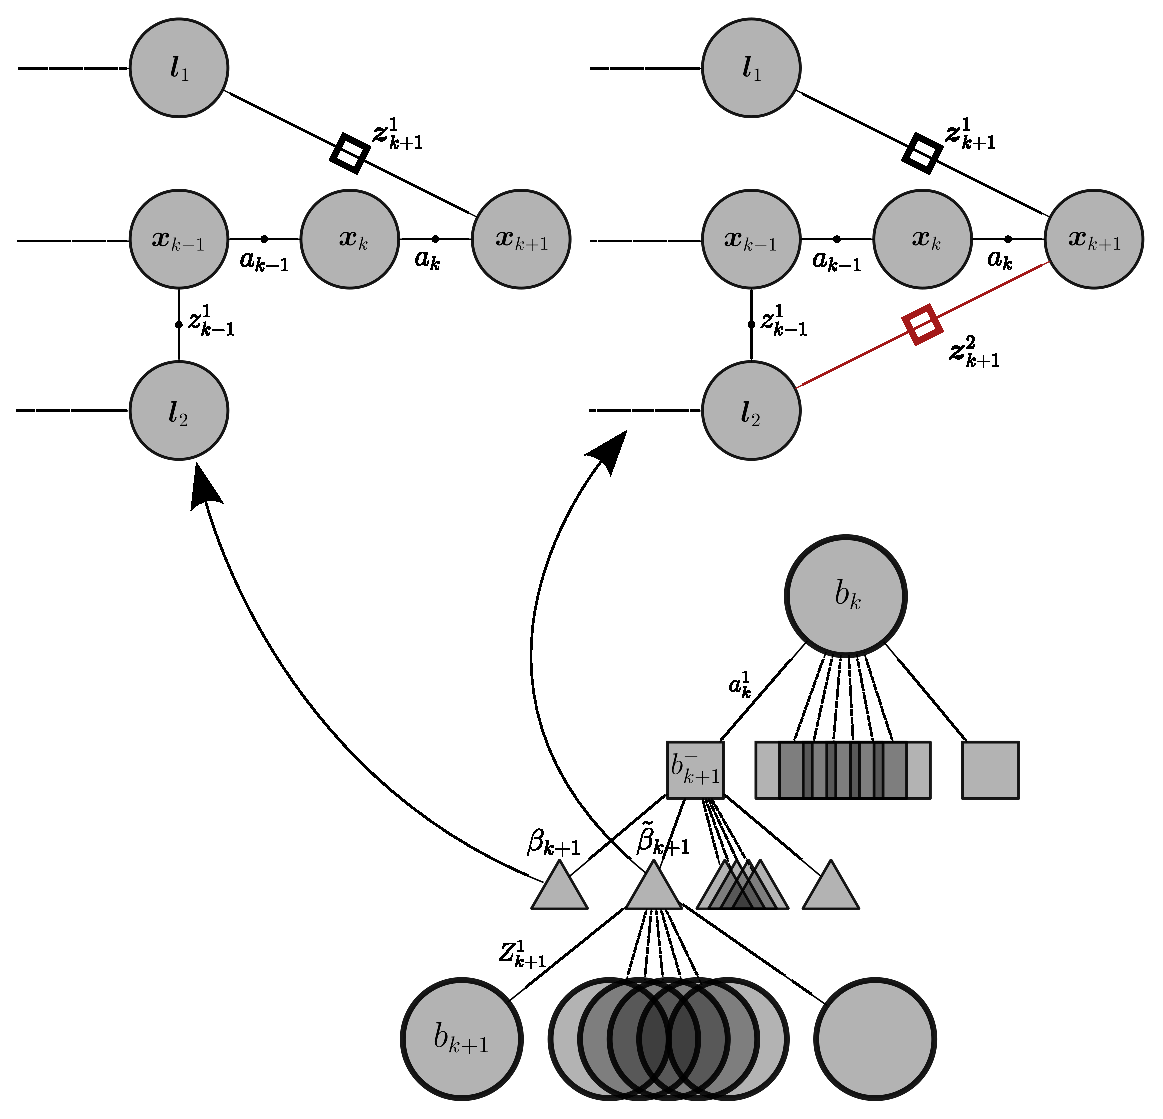
\includegraphics[width=0.4\linewidth,clip]{tree_to_topo.eps}
	\caption{Each da node (triangle) is associated with a specific factor graph topology. At this point the observations associated with the da realizations are still \glspl{rv}. In the example, by eliminating $\observationRV{k+1}{2}$, the topology resulting from $\tilde{\da{}{}}_{k+1}$ becomes identical to that of $\da{k+1}{}$}
	\label{fig:topology}
\end{figure}
High dimensional problems, such as \gls{slam}, often exhibit structure that allows for the belief to be represented via a factor graph. Planning algorithms that aim to address the problem of high-dimensional planning can thus leverage the topology of the problem as a cheap source of information. The comparison of topology between similar beliefs is captured by the \gls{da} variable ($\da{}{}$) as seen in \cref{fig:topology}. We assume that realizations of \gls{da} can be generated from the distribution $\probcond{\da{}{}}{\states{}}$ (e.g. a Bernoulli distribution on the failure rate of a locator beacon).

\subsection{Complete Factor Elimination}\label{sec:complete_elimination}

As illustrated in \cref{fig:topology}, the beliefs of neighboring \gls{da} nodes share much of the same topological aspects. More precisely, when $\norm{\da{}{}-\tilde{\da{}{}}}_{1}\ll\abs{L}$ and the history\footnote{When taking into account \gls{da}, $\hist{k}\triangleq\{\action{0:k-1},\da{1:k}{},\observations{1:k}\}$} $\priorHist{}$ is shared between the nodes (i.e., they share the same belief-action parent node), then the belief topology is identical up to
$\mathcal{F}\bigl(\abs{\tilde{\da{}{}}-\da{}{}}\bigr)$, where we recall that $f_i\in\mathcal{F}(\da{}{})$ is an observation factor as indicated by $\da{}{i}$. Although in this work we limit our discussion to a myopic comparison of \gls{da}, the concept can be extended to a non-myopic form. In the \gls{slam} scenario, $\da{}{}$ encodes the connectivity of pose to landmarks, with the observations yet unspecified (as is symbolized by the square nodes in the factor graphs of \cref{fig:topology}). This similarity in the topology motivates the removal of selected \gls{da} nodes, with guarantees in the form of bounds formulated as a function of the remaining \gls{da} nodes. We examine \cref{thm:general_bounds} in its application to \eqref{eq:da_bellman} to understand the potential method for eliminating specific realizations of \gls{da}.
\begin{equation}
	\label{eq:remove_da}
	\expectation{\expectation{V^\pi(\blf{})}{\observationsRV{}\mid\daRV{}{}}}{\daRV{}{}}-\partialexpectation{\expectation{V^\pi(\blf{})}{\observationsRV{}\mid\daRV{}{}}}{\subSpace}=\sum_{\da{i}{}\in\stcomp{\subSpace}}\measure{\da{i}{}}\expectation{V^\pi(\blf{})}{\observationsRV{}\mid\da{i}{}}\;.
\end{equation}
where $\subSpace\subseteq\mathcal{D}$.

\Cref{eq:remove_da} is an equality as we have not yet bounded the expected value function. The next step is to bound the conditional expectation.

\subsection{Application to Conditional Entropy}

For an application of eliminating realizations of \gls{da}, we look to conditional entropy as our expected reward. \Cref{thm:entropy_bounds} forms the basis of our bounds, but it does not take into consideration different \glspl{da}. This brings us to our novel bound on the conditional entropy that takes advantage of the problem topology in order to make high-dimensional planning more tractable.

\begin{corollary}
	\label{thm:bounds_elim}
	$\lowerbound(\da{\textup{diff}}{})\leq\condEntropy{\statesRV{}}{\observationsRV{},\tilde{\da{}{}}}-\simplecondEntropy{\statesRV{}}{\observationsRV{},\da{}{},\tilde{\da{}{}}}{}\leq\upperbound(\da{}{},\tilde{\da{}{}})\quad\forall\tilde{\da{}{}},\da{}{}\in\mathcal{D}$, where:
	\begin{small}
		\begin{subequations}
			\begin{align}
				\lowerbound(\da{}{},\tilde{\da{}{}}) & =-\sum_{f_i\in\mathcal{F}(\da{\textup{diff}}{})}\left(\log\sup M_{f_i}-\log m_{\norm{f_i}}\right)-\upperbound_{\da{}{\prime}}\Bigl(\expectation{\log C_{pm}}{\observationsRV{}}\Bigr)\;,\\
				\upperbound(\da{\textup{diff}}{}) & =-\sum_{f_i\in\mathcal{F}(\da{\textup{diff}}{})}\left(\log\inf m_{f_i}-\log M_{\norm{f_i}}\right)\;,\\
				\simplecondEntropy{\statesRV{}}{\observationsRV{},\da{}{},\tilde{\da{}{}}}{}&\triangleq\entropy{\statesRV{}} +\E_{\observationsRV{}{}\mid\da{}{\prime}}\Biggl[{\log\Big\lVert{\prob{\states{}}\prod_{f_i\in\mathcal{F}(\da{}{\prime})}f_i}\Big\rVert_{q}^{\states{}}}\Biggr]\;,
			\end{align}
		\end{subequations}
	\end{small}
	$\da{\textup{diff}}{i}\triangleq\max(\tilde{\da{}{i}}-\da{}{i},0)$, $\da{}{\prime}\triangleq\tilde{\da{}{}}-\da{\textup{diff}}{}$ and	$\upperbound_{\da{}{\prime}}\Bigl(\expectation{\log C_{pm}}{\observationsRV{}}\Bigr)$ is defined in the proof.
\end{corollary}
\begin{proof}
	From \autoref{thm:entropy_high_dim_bounds}, if we take the global extremes and completely eliminate the observations we trivially arrive at the desired statement.

	For this case:
	\begin{equation*}
		\begin{split}
			\upperbound_{\da{}{\prime}}\left(\expectation{\log C_{pm}}{\observationsRV{}}\right)&=-\frac{m\log p}{p}-\frac{\log q}{q}-\sum_{f_i\in\mathcal{F}(\da{\textup{diff}}{})}\log \inf m_{f_i}-\expectation{\log m_{\states{}}}{\observationsRV{}{}\mid\da{}{\prime}}\\
			&\phantomeq+\E_{\observationsRV{}{}\mid\da{}{\prime}}\left[\log\left(\sum_{f_i\in\mathcal{F}(\da{\textup{diff}}{})}\left(\sup M_{f_i}\right)^{p-1}\inf m_{f_i}+M_{\states{}}^{q-1}m_{\states{}}\right)\right]\;,
		\end{split}
	\end{equation*}
	where
	\begin{align*}
		&M_{f_i}\triangleq\sup_{\states{}}\probcond{\observationRV{i}{}}{\states{}}\;,&&
		m_{f_i}\triangleq\inf_{\states{}}\probcond{\observationRV{i}{}}{\states{}}\;,
		\\
		&M_{\states{}}\triangleq\sup_{\states{}}\prod_{f_i\in\mathcal{F}(\da{}{\prime})}f_i\prob{\states{}}\;,&&
		m_{\states{}}\triangleq\inf_{\states{}}\prod_{f_i\in\mathcal{F}(\da{}{\prime})}f_i\prob{\states{}}\;.
	\end{align*}
\end{proof}

It should be noted that for the bounds to be meaningful, $\inf m_{f_i}>0$. For example, this is not the case when $f_i$ is the Gaussian distribution. Furthermore, this limits the discussion of $f_i$ to finite support.

As an example let us assume $\tilde{\da{}{}}=\begin{bmatrix}1&1&0\end{bmatrix}^\intercal$ and $\da{}{}=\begin{bmatrix}0&1&1\end{bmatrix}^\intercal$. For such a case we find that $\da{\textup{diff}}{}=\begin{bmatrix}1&0&0\end{bmatrix}^\intercal$ and $\da{}{\prime}=\begin{bmatrix}0&1&0\end{bmatrix}^\intercal$. We note that $\da{}{\prime}$ indicates as to what associations are shared between $\tilde{\da{}{}}$ and $\da{}{}$. We provide the equivalent definitions $\da{}{i\prime}\equiv \tilde{\da{}{i}}\land\da{}{i}$ and $\da{\textup{diff}}{i}\equiv \tilde{\da{}{i}}\land\lnot\da{}{i}$.
When $\tilde{\da{}{}}\succeq\da{}{}$, $\da{}{\prime}\equiv\da{}{}$ and when $\tilde{\da{}{}}\preceq\da{}{}$, $\da{\textup{diff}}{}=0$ resulting in no computational benefit, as the computational benefit is proportional to $\norm{\da{\textup{diff}}{}}_1$. This highlights the trade-off between computational efficiency and tightness of the bounds when selecting a $\da{}{}\in\subSpace$ for the computation of \autoref{thm:bounds_elim}.

To incorporate \autoref{thm:bounds_elim} into planning, the bounds must be applied in the context of the value function. As shown, the bounds are myopic and bound the immediate expected reward. \autoref{thm:val_func_immediate_bounds_obs_bellman} allows for bounding the value function with respect to bounds on the immediate expected reward. In a similar fashion we can bound the expected value function as shown in \eqref{eq:remove_da}, where now different realizations of \gls{da} are taken into consideration.

We are unaware of prior works that provide bounds on the value function while considering different \gls{da} realizations, when the reward is the entropy of the state. In~\cite{Shienman22icra} the authors consider the Shannon entropy of the hypothesis probabilities. In~\cite{Yotam24tro} the authors consider simplification of the observation space for the expected differential entropy for a given \gls{da}.
\chapter{Experiments}
\section{Low Dimensional Reward Bounds}
\subsection{Simulation Setup}
\begin{figure}[h]
	\centering
	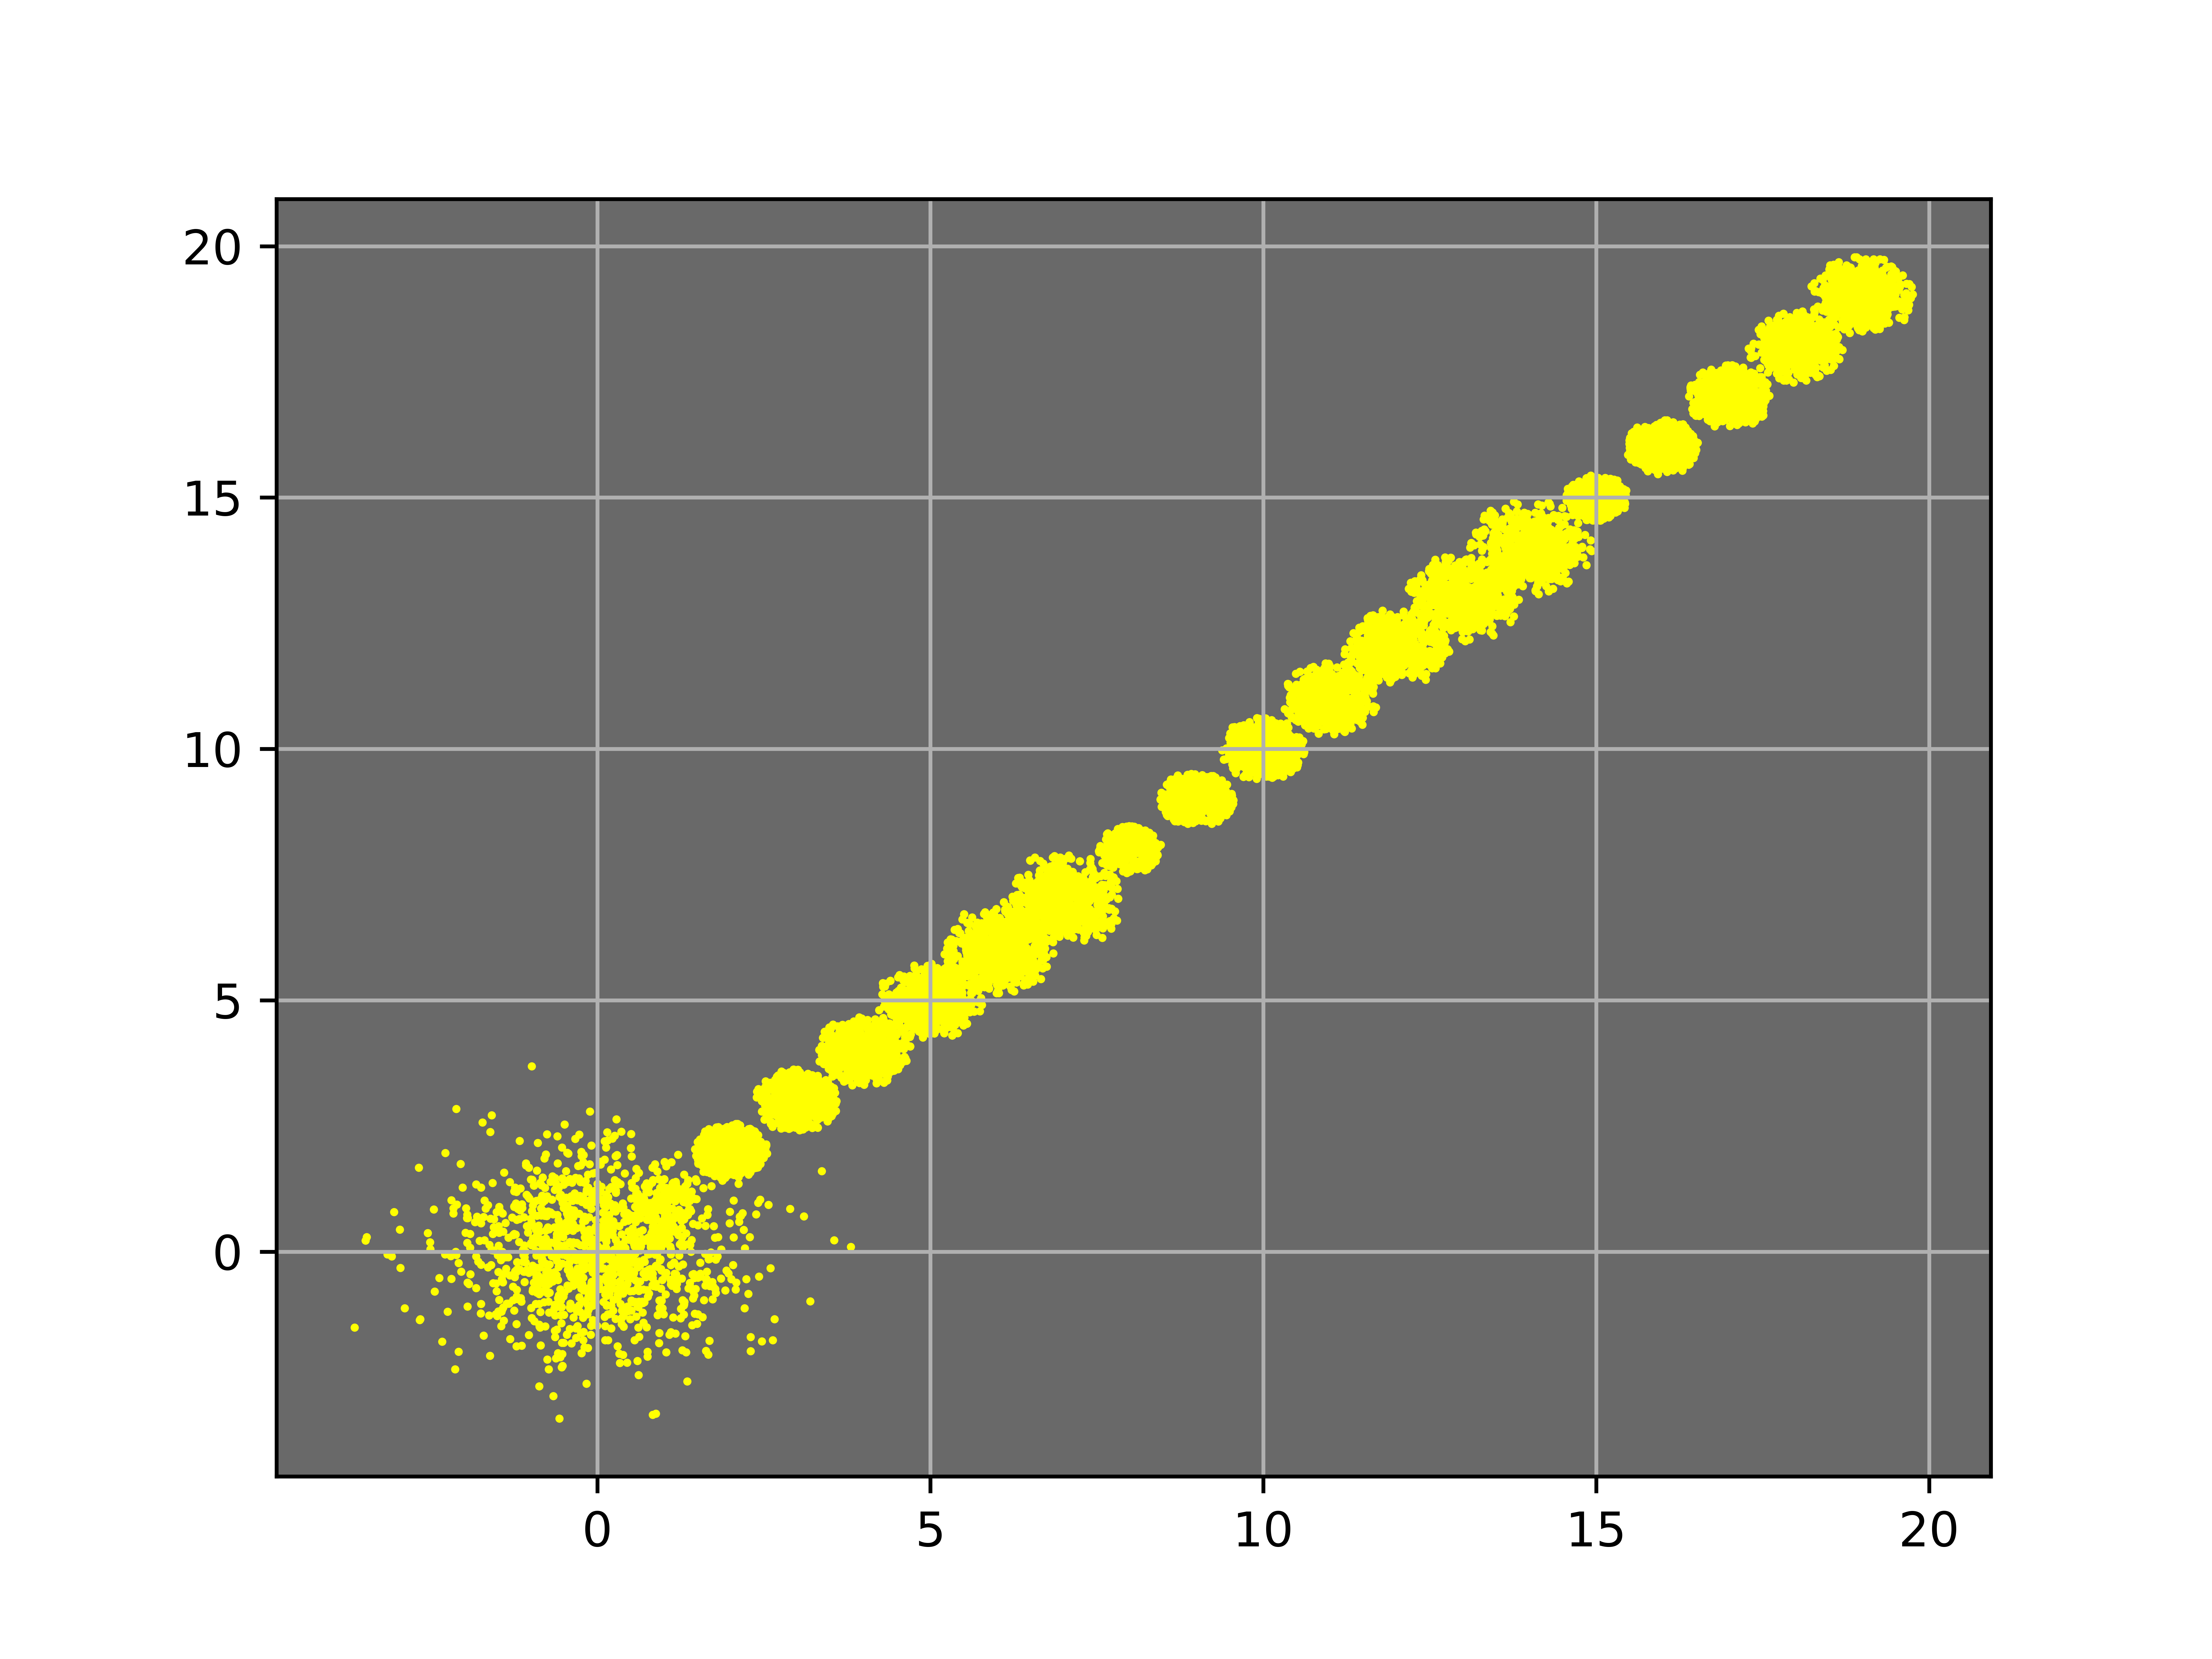
\includegraphics[width= 0.4\linewidth,clip]{belief_trajectory}
	\caption{The trajectory of the particle filter over time. The action taken each time-step is $[1,1]$.}
	\label{fig:belief_trajectory}
\end{figure}
	We begin our empirical study in a low dimensional particle filter scenario. The agent is given to be in $\mathbb{R}^2$, and we begin with a prior belief $\blf{0}\sim N(0,I\sigma_0^2)$. The agent is moved along a predetermined trajectory for which it is given a transition model upon which to perform predictions of the form $\state{}^\prime=\state{}+\action{}+\omega_{\action{}}$ where $\omega_{\action{}}\sim N_{r_a}(0,I\sigma_{\action{}}^2)$. The agent also gathers noisy measurements along its path $\observation{}{}=\state{}+\omega_{\observation{}{}}$, where $\omega_{\observation{}{}}\sim N_{r_{\observation{}{}}}(0,I\sigma_{\observation{}{}}^2)$ and the observation noise is time dependent. $N_{r}(0,\Sigma)$ is a multivariate zero-mean Gaussian distribution with covariance $\Sigma$ and truncated at radius $r$, allowing for an infimum greater than zero, which is reasonable given noise filtering and outlier pruning practices. The belief is maintained as a set of weighted particles $\{\states{}^i,\weight{}{i}\}_{i=1}^N$ and we use a particle filter to update the belief each time-step. The reward is an estimator of the entropy given by~\cite{Boers10fusion}. At the end of each update step particles with zero weight were discarded (possible because of the truncated Gaussian), after reward calculation resampling was performed. The trajectory of the particle filter can be seen in \cref{fig:belief_trajectory}. We evaluate our bounds \autoref{thm:boers_bounds_simple} and compare them to those provided by~\cite{Sztyglic22iros}.
\subsection{Results}
\begin{figure}[h]
	\centering
	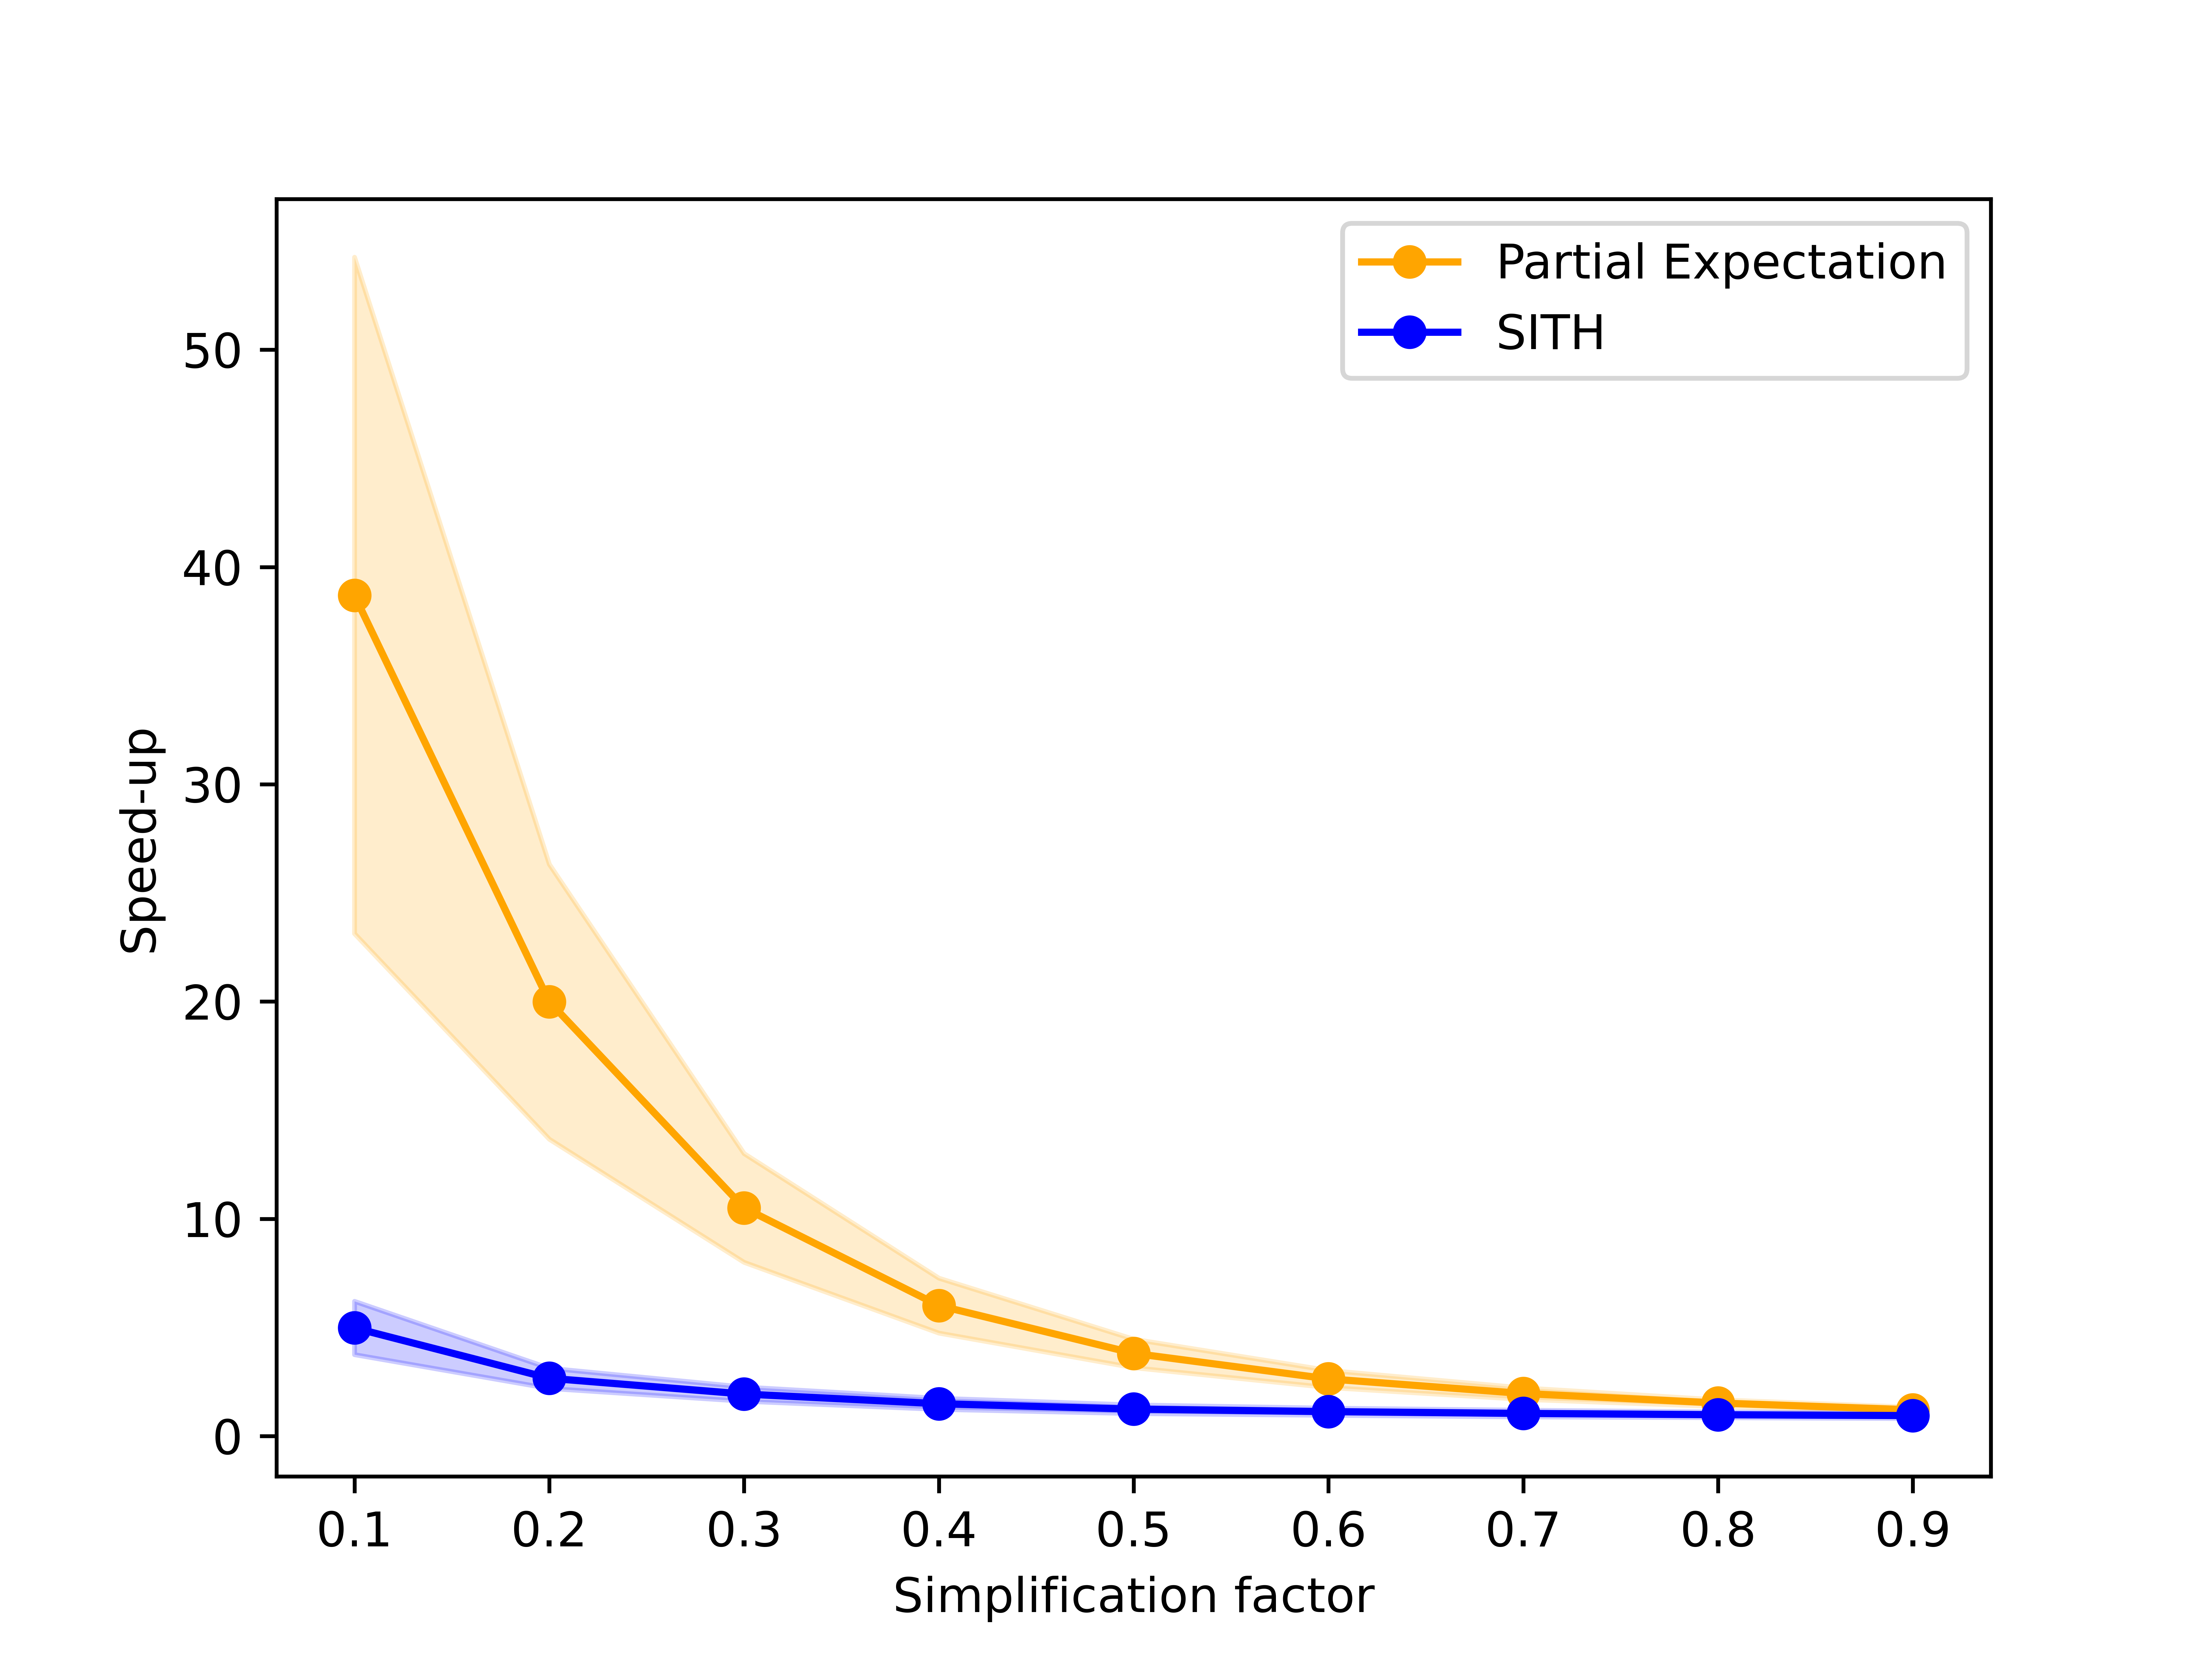
\includegraphics[width= 0.4\linewidth,clip]{speedup}
	\caption{The relative speed-up of each bounding algorithm on the Boer's estimator, speed-up is relative to the Boer's estimator time. Results are averaged over 10 runs using a nominal set of 1000 belief particles.}
	\label{fig:speedup}
\end{figure}
	In our comparison there are two primary aspects which we would like to investigate. This first is the relative computational efficiency of each algorithm, and the second is the bound tightness. Beginning with the computational efficiency, the Boer's estimator requires $O(N^2)$ computations. We define $\alpha = n/N$ to be the simplification factor, as such the computational complexity of the SITH bounds are $\alpha_sN^2$ and the complexity of our bounds are $\alpha_p^2N^2$ for $0<\alpha\leq1$. Thus for the same level of simplification, we expect a quadratic speed-up, whereas the SITH bounds are limited to a linear speed-up. If we look at \cref{fig:speedup} we observe this exact behavior. Furthermore, as the SITH algorithm also makes use of computations on the complementary set of particles is complexity has some added linear complexity with respect to $N$, this is often observed at large values of $\alpha$ where there is not much simplification. For example, for $\alpha_s=\numlist{0.8;0.9}$ the relative speed-up is less than 1, meaning that calculating the bounds is more computationally expensive.
\begin{figure} [h]
	\centering
	\begin{subfigure}[t]{0.32\textwidth}
		\centering
		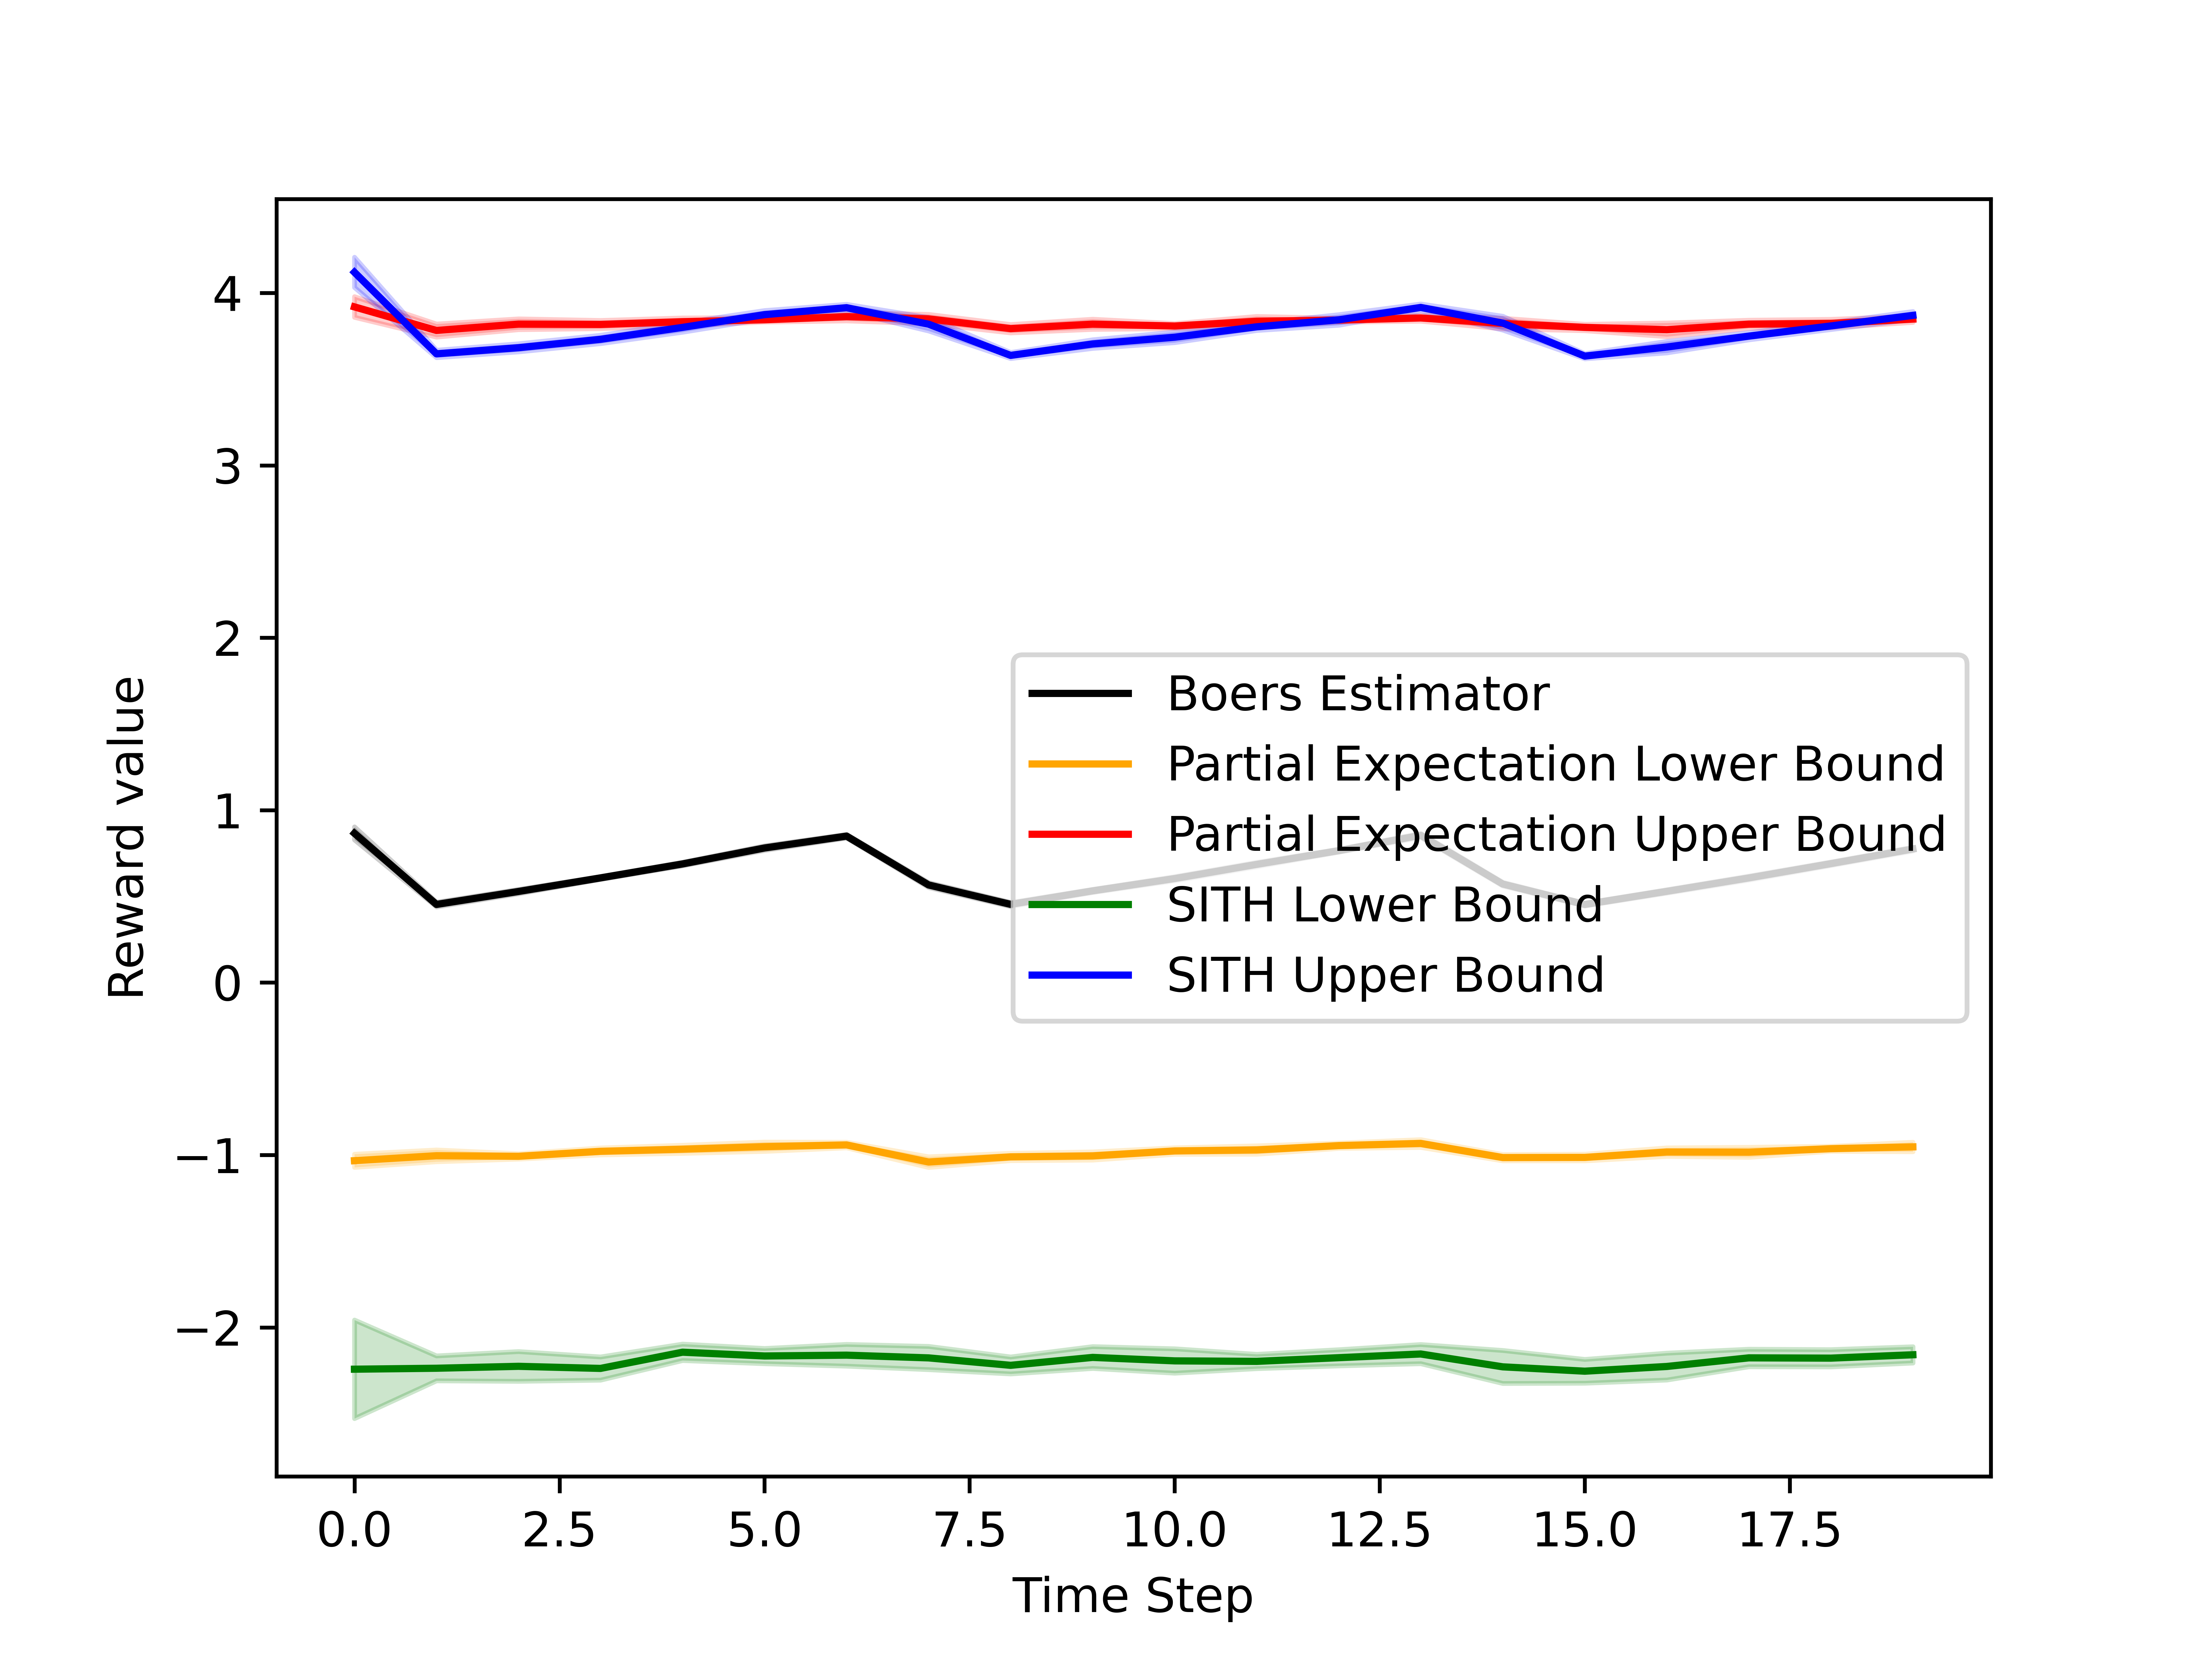
\includegraphics[width= 0.95\linewidth,clip]{1200_03}
		\caption{$\alpha_p=0.3$, relative speed-up of \num{11.0\pm2.7} for partial expectation and \num{5.8\pm1.5} for SITH}
		\label{fig:alpha_03}
	\end{subfigure}
	\hfill
	\begin{subfigure}[t]{0.32\textwidth}
		\centering
		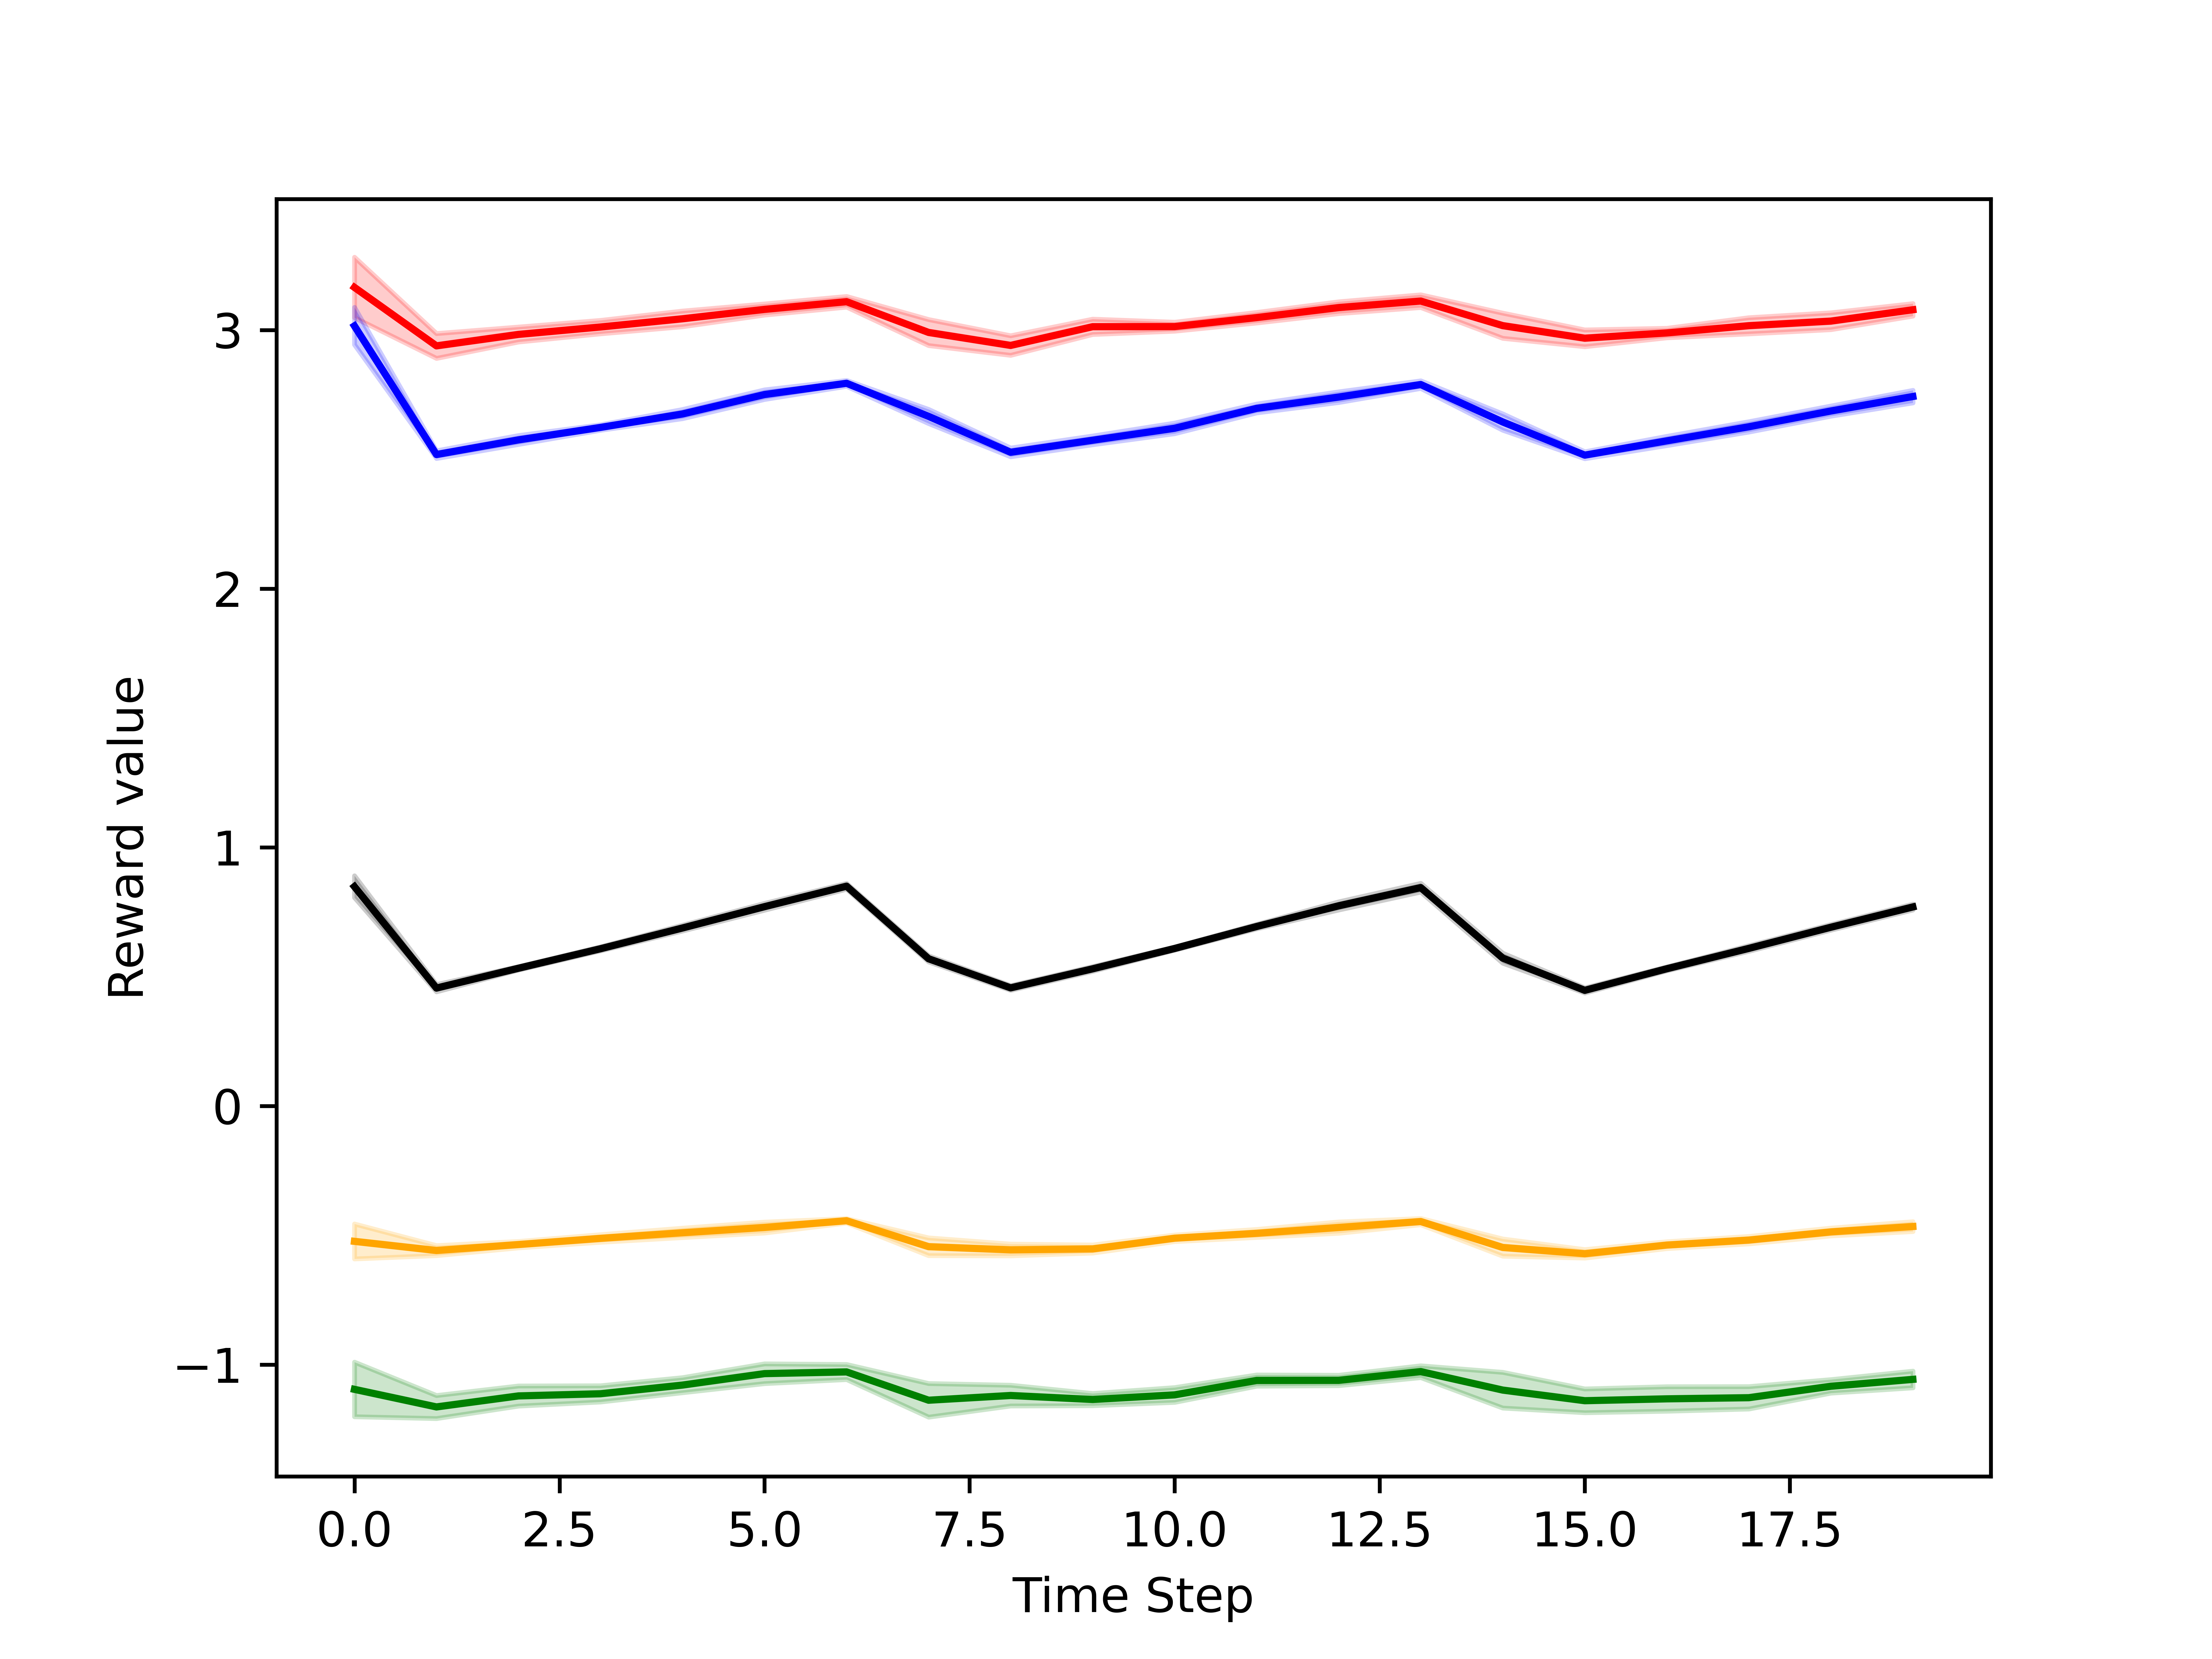
\includegraphics[width= 0.95\linewidth,clip]{1200_05}
		\caption{$\alpha_p=0.5$, relative speed-up of \num{3.6\pm0.5} for partial expectation and \num{2.0\pm0.3} for SITH}
		\label{fig:alpha_05}
	\end{subfigure}
	\hfill
	\begin{subfigure}[t]{0.32\textwidth}
		\centering
		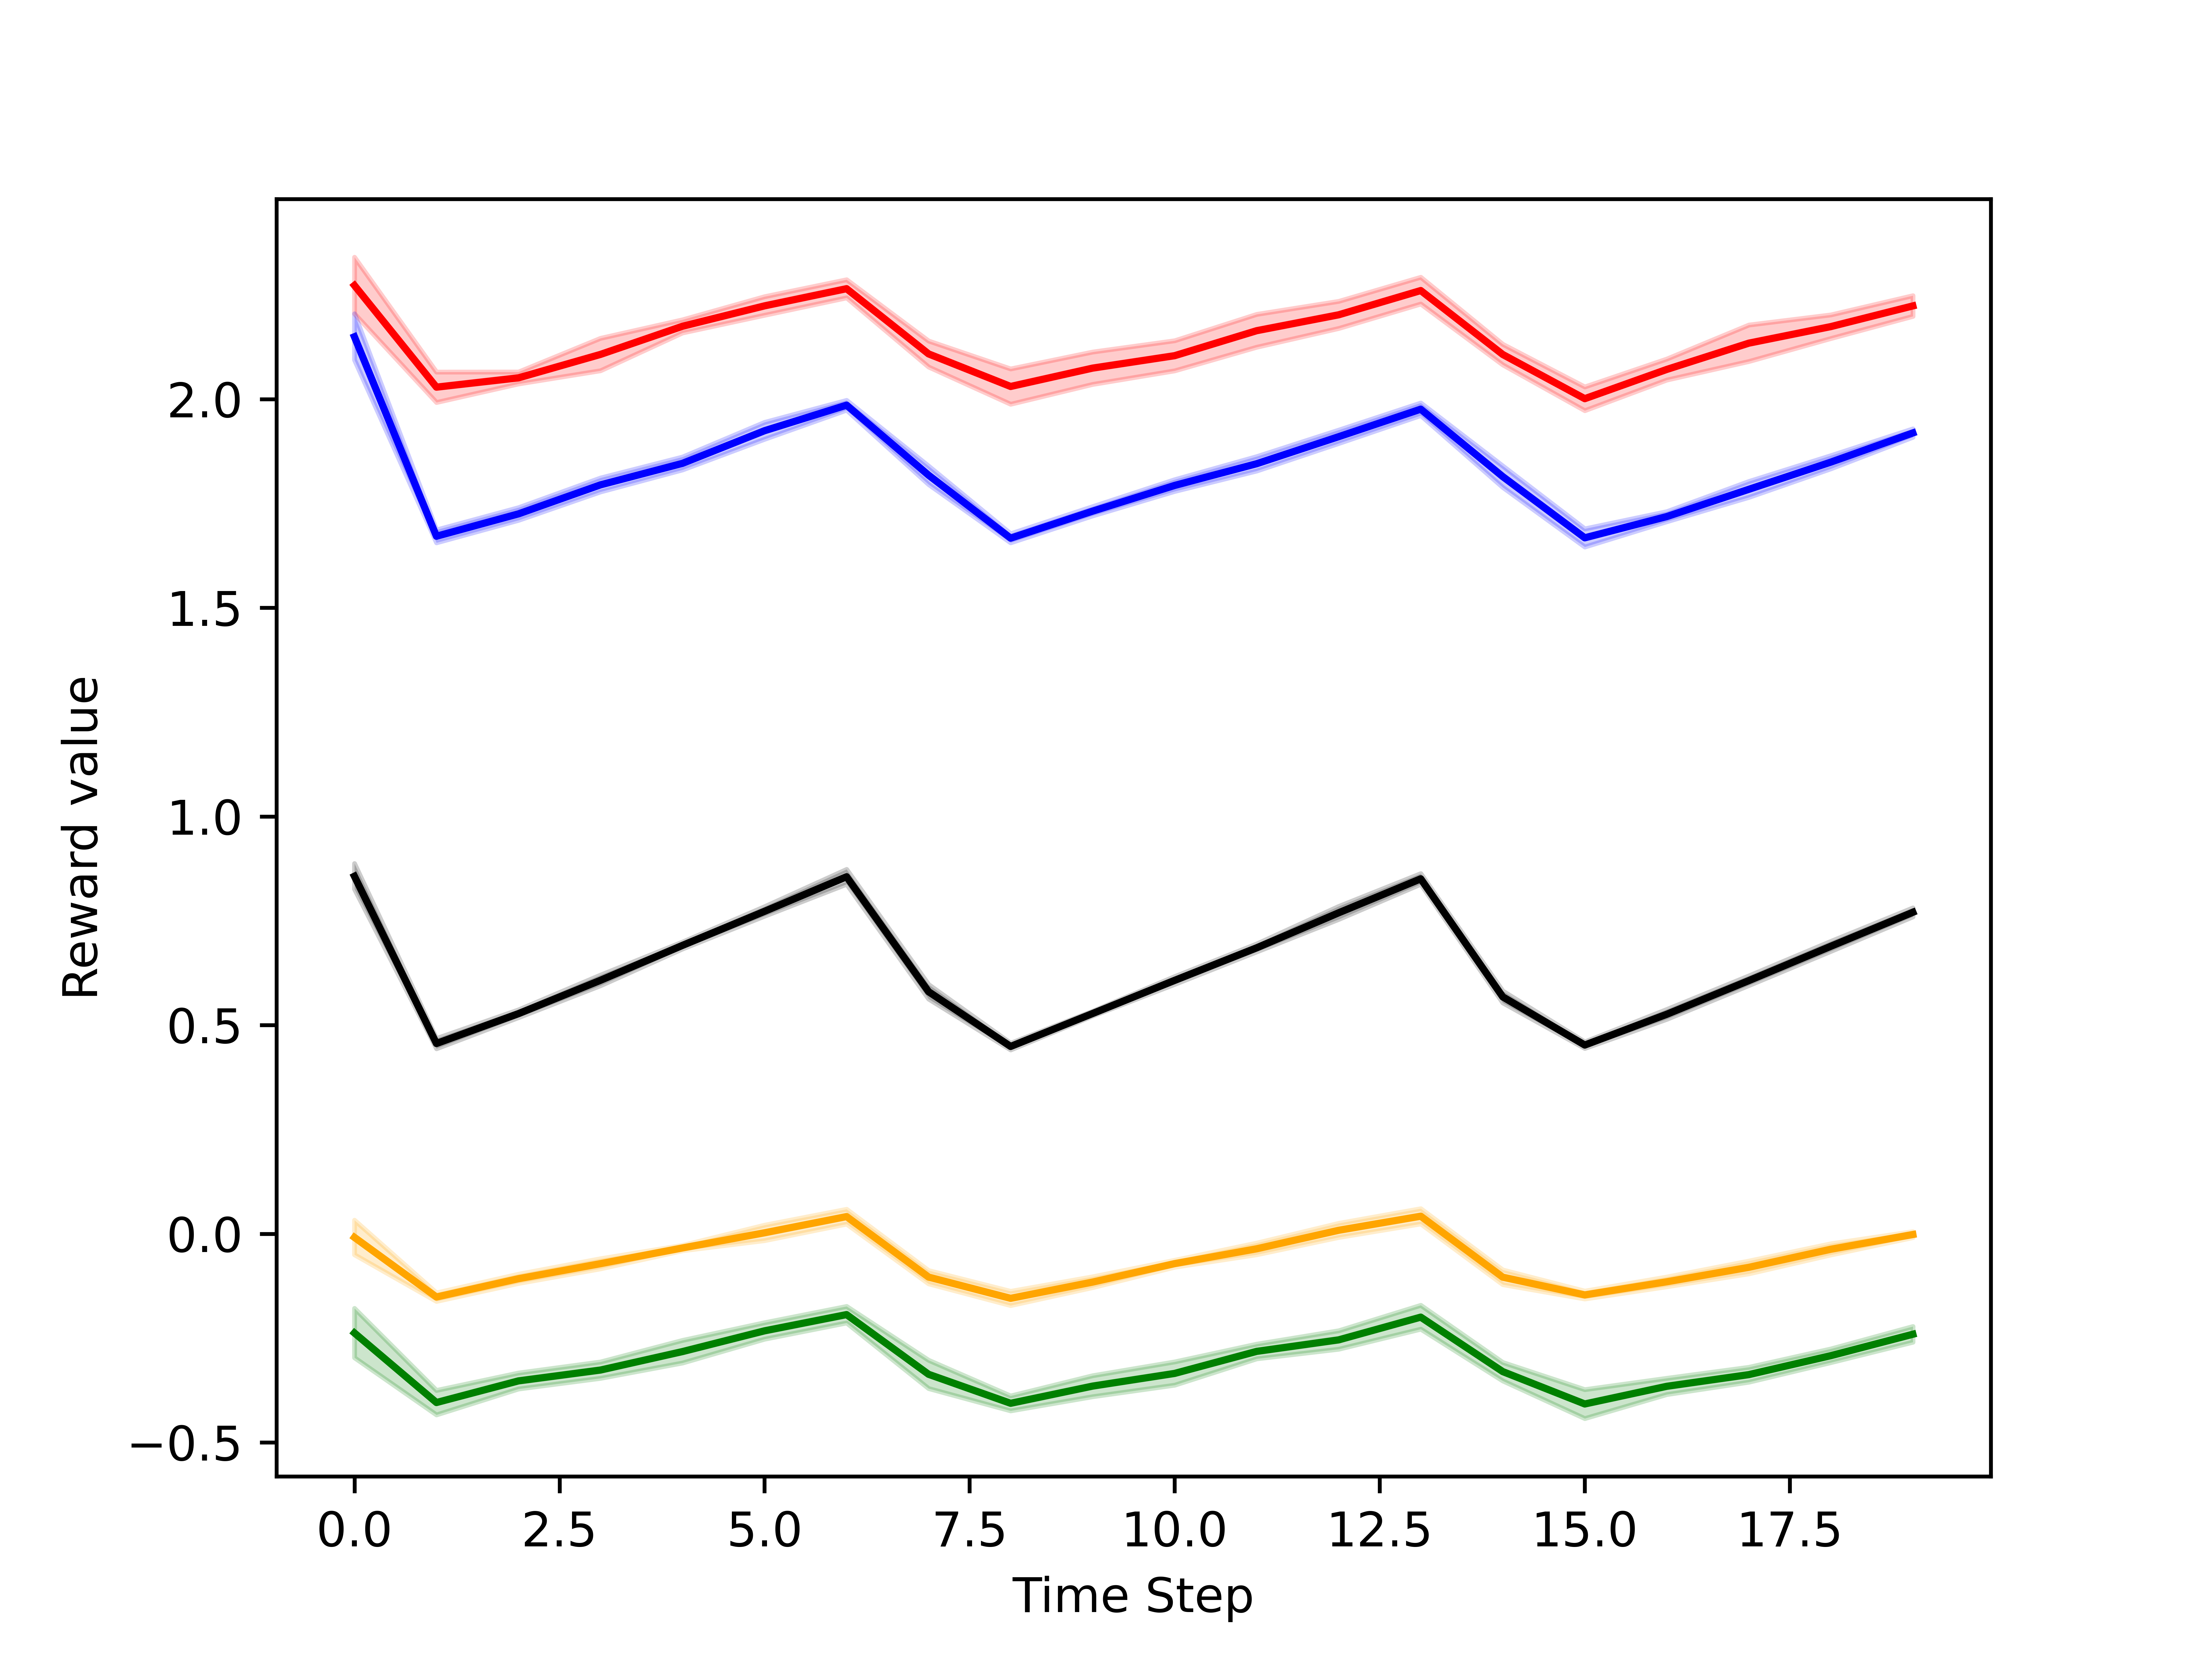
\includegraphics[width= 0.95\linewidth,clip]{1200_07}
		\caption{$\alpha_p=0.7$, relative speed-up of \num{1.9\pm0.2} for partial expectation and \num{1.2\pm0.2} for SITH}
		\label{fig:alpha_07}
	\end{subfigure}
	\caption{Bounds on the Boer's estimator for $\alpha_s=\alpha_p^2$, averaged over 10 runs using a nominal 1200 belief particles.}
	\label{fig:boers_bound_comp}
\end{figure}
	From \cref{fig:boers_bound_comp}\footnote{The periodic nature of the plots is a results of the periodic definition of the observation covariance in the simulations which can be noticed in \cref{fig:belief_trajectory}.} it is apparent that as $\alpha$ shrinks both bounds become looser, as is expected, but that the bounds of SITH loosen more than our bounds. In all cases our lower bound outperforms that of SITH. With respect to the upper bound, as we use less particles in the bound calculations, we note that our bounds begin to outperform those of SITH. In these simulations we defined $\alpha_s=\alpha_p^2$ and use the same $n$ particles between bounds. The idea was to keep the speed-up constant between the algorithms and compare for bound tightness. What we see though is that even though the same particles are used, our bounds still outperform those of SITH with respect to speed-up, almost by a factor of two at times, while supplying comparable bounds, if not better. Finally we would like to note that for larger values of $\sigma_{\observation{}{}}$ (we found this to be about $\sigma_{\observation{}{}}>r_{\action{}}+r_{\observation{}{}}$), the SITH upper bound would becomes superfluous, returning $\infty$. This is due to the upper bound of $(b)$ in Theorem 3. of~\cite{Sztyglic22iros} which is a summation of the transition likelihood between a subset of prior particles and all propagated particles. As we use a particle filter, nothing ensures that a propagated particle will have a prior particle with non-zero transition likelihood because of the truncated Gaussian. This problem is avoided in our bounds as the summation is between a subset of prior particles and the propagated subset itself.
\section{High Dimensional Planning}
\subsection{Simulation Setup}
\begin{figure}[h]
	\centering
	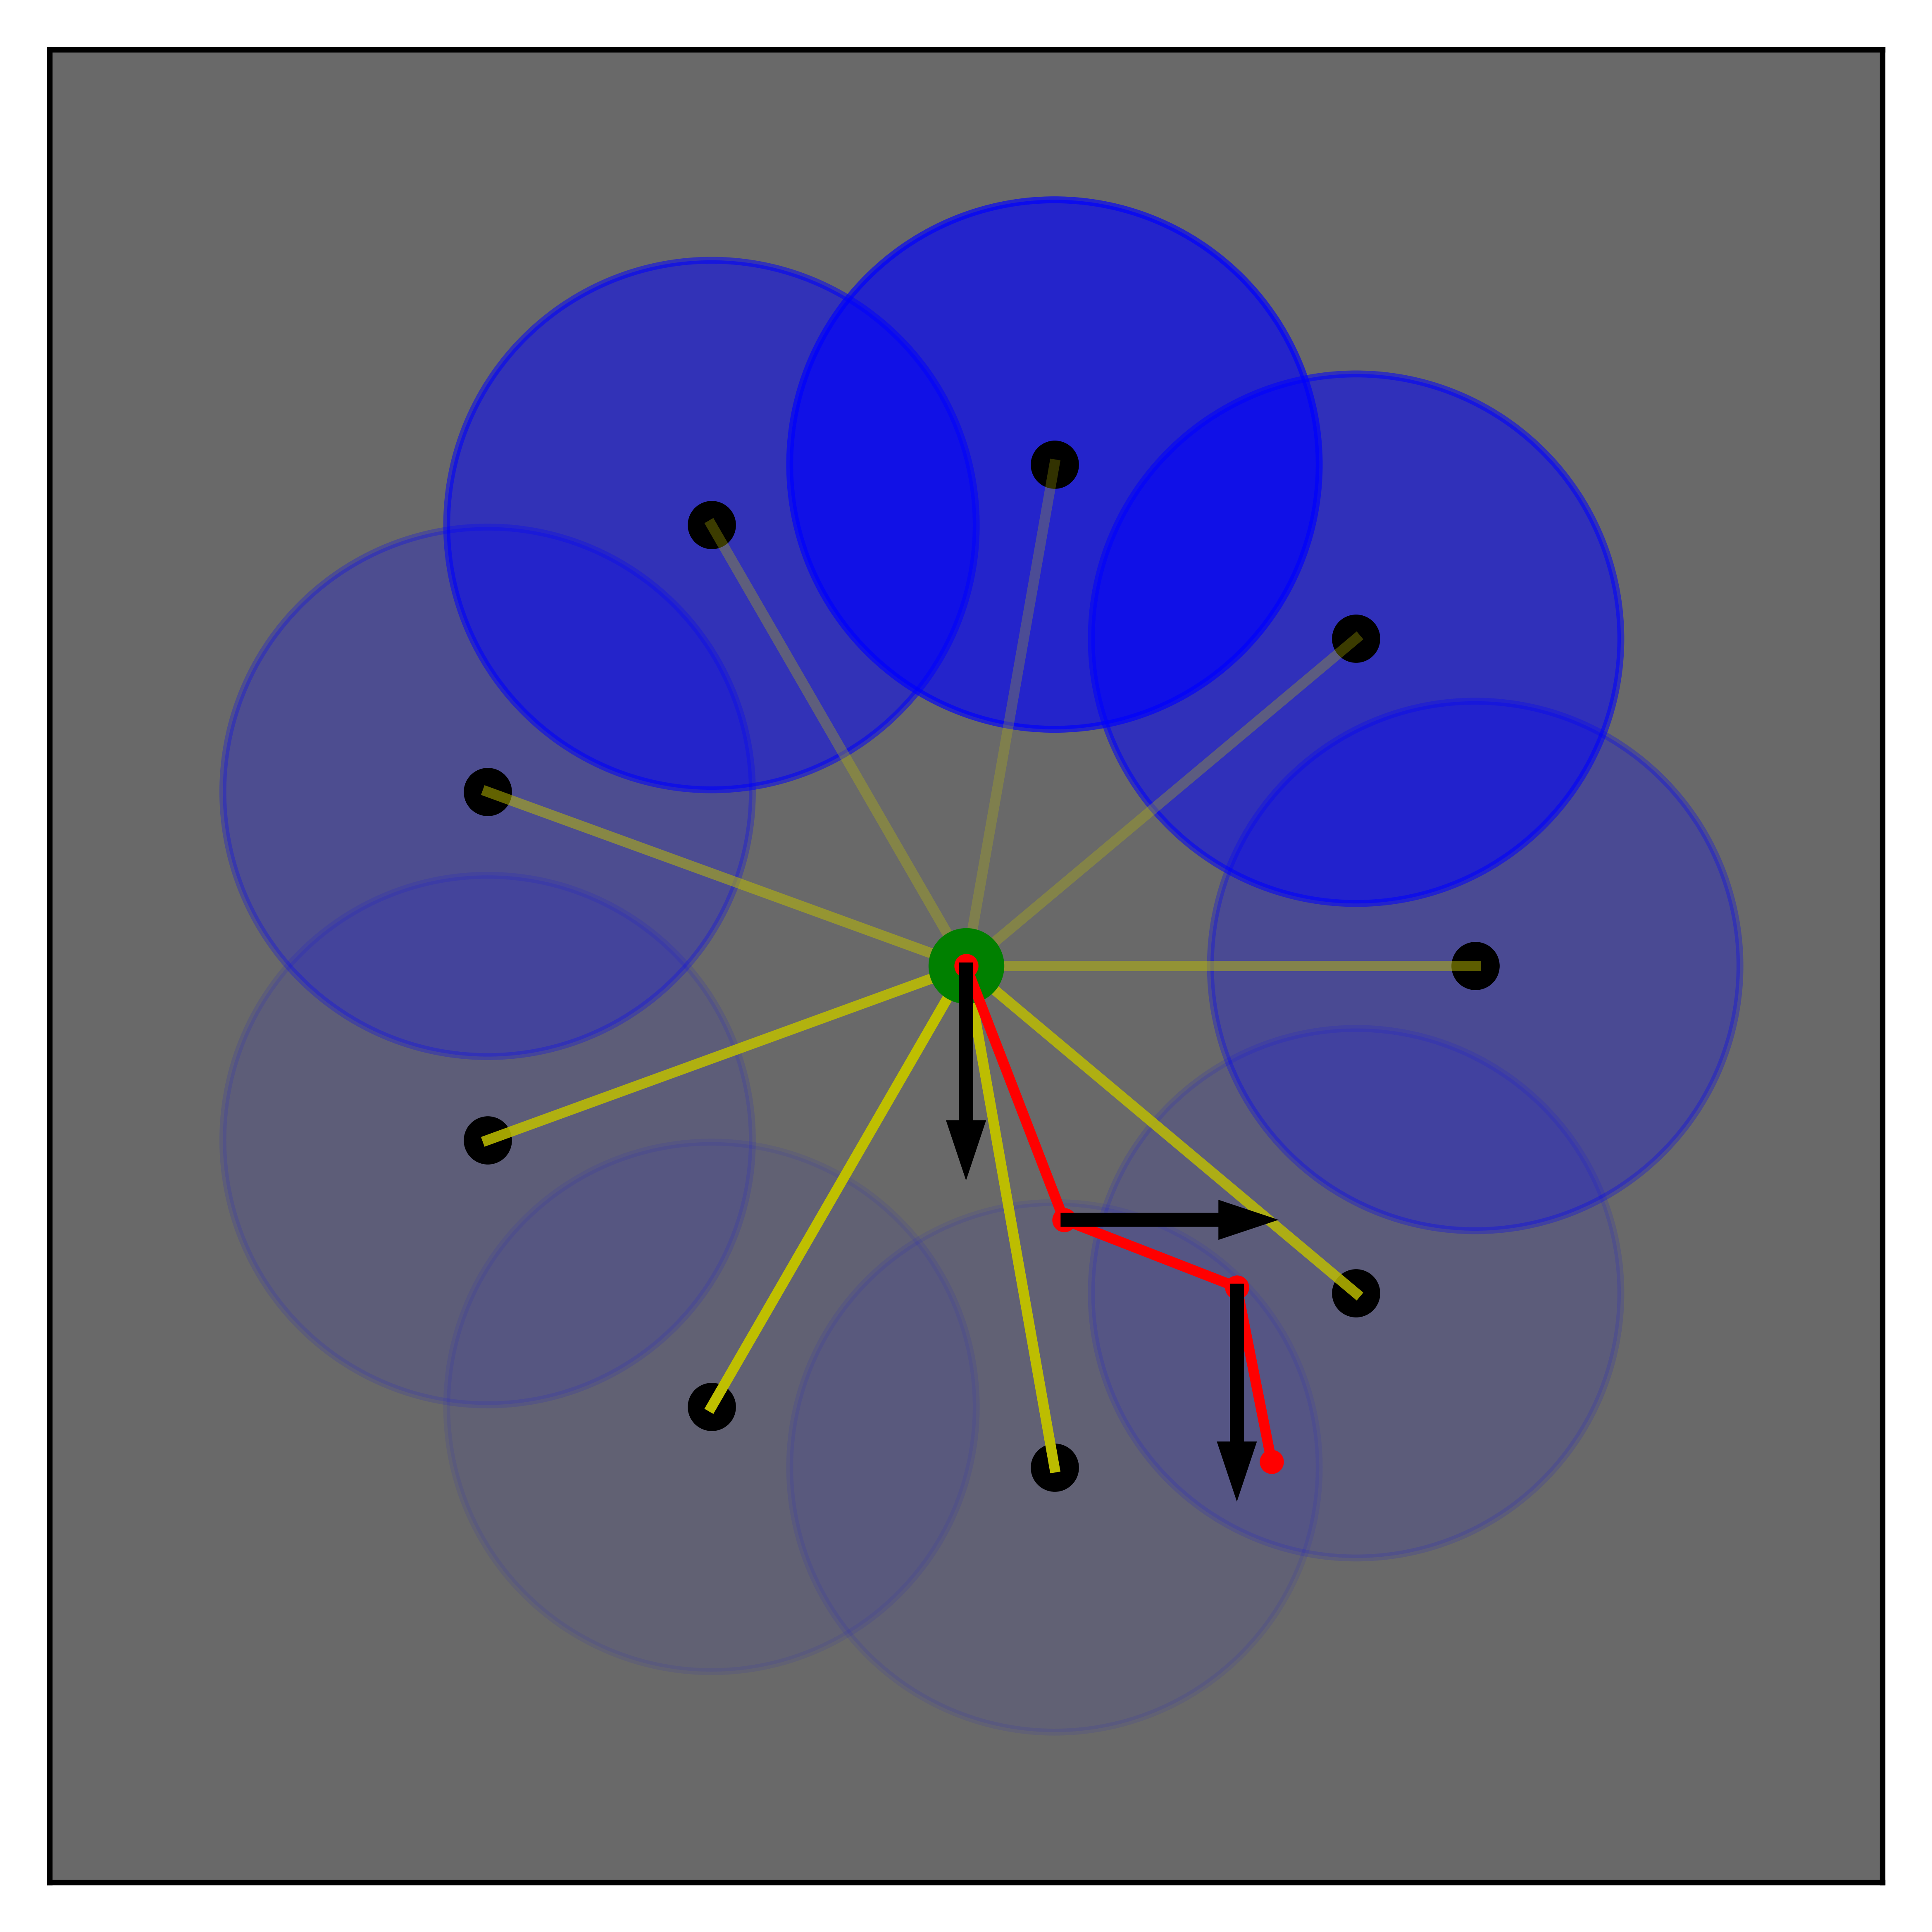
\includegraphics[width= 0.4\linewidth,clip]{actions}
	\caption{The agent path as dictated by the optimal actions, overlayed with the actions selected by the maximum lower bound on the Q-function for $\kappa=0.5$. In this case the maximum lower bound was in agreement with the optimal action, this is not always the case. The beacon intensity denotes its probability of success. And the line intensities are directly proportional to the covariance of the observation factor used as an initial belief.}
	\label{fig:actions}
\end{figure}
As discussed in \cref{sec:complete_elimination}, \autoref{thm:bounds_elim} can be utilized alongside \eqref{eq:remove_da} when formulated for expected reward. The following simulations demonstrate the improvement in runtime and the resulting bounds obtained upon utilizing the aforementioned inequalities.

We consider planning in the landmark-\gls{slam} scenario, a high-dimensional smoothing problem where the state space expands over time to include current and past poses, as well as landmarks in $\mathbb{R}^2$. The action space consists of unit circle motion primitives. The transition model is given by $\state{}^\prime=\state{}+\action{}+\omega_{\action{}}$ where $\omega_{\action{}}\sim N_{r_a}(0,I\sigma_{\action{}}^2)$, and the observation model is given by $\observation{}{}=\landmark{}-\state{}+\omega_{\observation{}{}}$, where $\omega_{\observation{}{}}\sim N_{r_{\observation{}{}}}(0,I\sigma_{\observation{}{}}^2)$. Observations are relative position between poses and landmarks. Each landmark $\landmark{i}$ has probability $p_i$ to succeed in sending an observation to the agent once the agent is within a radius $r$ of the landmark (i.e. $\probcond{\da{}{i}}{\state{},\landmark{i}}=\1{\norm{\state{}-\landmark{i}}\leq r}p_i$). The reward is given to be negative entropy as the task is information gain.

An initial belief over the agent pose and landmarks is instantiated via a prior on the initial pose and observation factors to each landmark. Subsequently belief tree is constructed using sparse sampling, where, in addition to action and observation nodes, we introduce \gls{da} nodes (see \cref{fig:topology}). High-dimensional inference is handled incrementally using the slices approach from~\cite{Shienman24arxiv}. After constructing the tree in a downward pass, rewards, expected reward bounds, and Q-functions are calculated in an upward pass while maintaining Bellman optimality. In the case of bounds on the Q-function, the maximum over the lower and upper bounds are passed up. We define $\kappa$ as $\frac{\abs{\subSpace}}{\abs{\mathcal{D}}}$, representing the proportion of \gls{da} nodes eliminated for the expected reward bounds.  When $\kappa=1$ no nodes are eliminated and the expected reward remains unchanged; for $\kappa=0$ all $\da{}{}$ realizations are discarded, resulting in loose bounds on the expected reward. Specifically, $\kappa$ splits $\mathcal{D}$ into two sets: $\da{}{}\in\subSpace$ and $\tilde{\da{}{}}\in\stcomp{\subSpace}$ as required for \autoref{thm:bounds_elim}. The reference \gls{da}, $\da{}{}$, is used to calculate bounds on $\condEntropy{\statesRV{}}{\observationsRV{},\tilde{\da{}{}}}$; the selection process of a reference \gls{da} is not addressed in this work, and we simply select a reference \gls{da} such that $\da{\textup{diff}}{}\neq0$. Joint state sampling via~\cite{Shienman24arxiv} allows access to the estimated joint likelihood which was used to evaluate the reward. The weighted samples represent our belief over the state for reward calculations, using the same samples for both rewards and bounds.

\subsection{Results}
\begin{figure}[h]
	\centering
	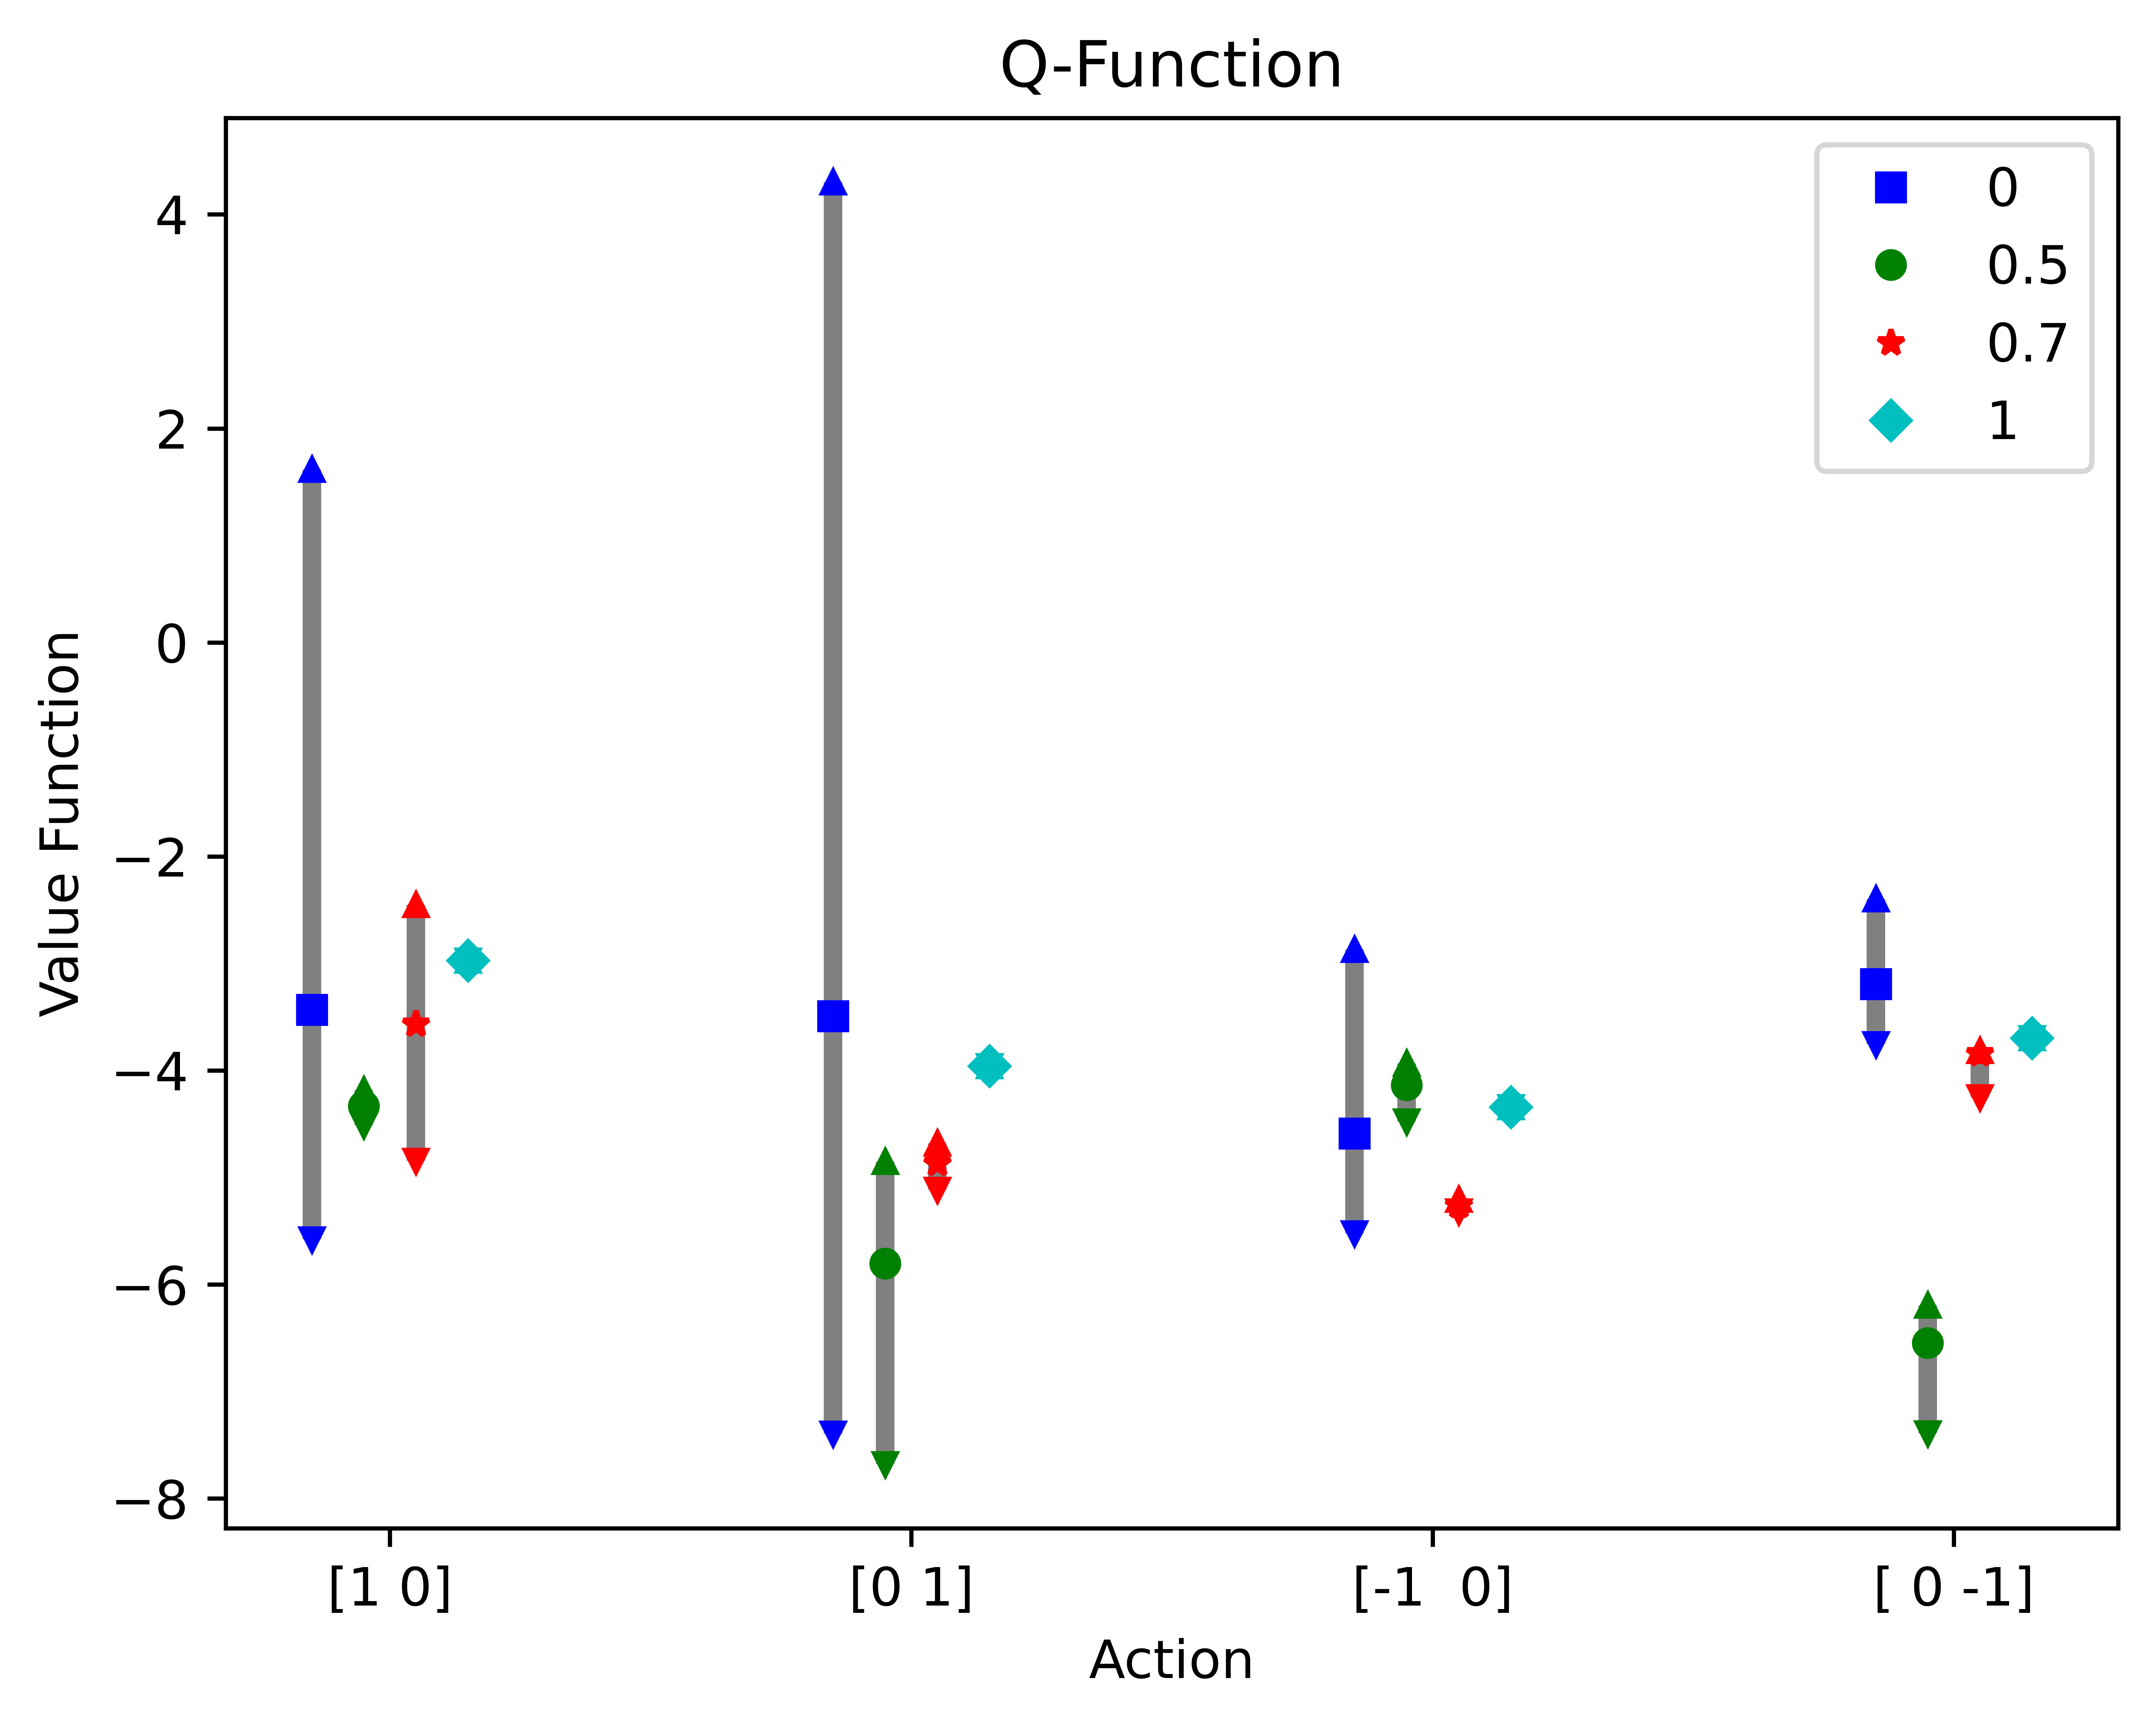
\includegraphics[width= 0.4\linewidth,clip]{q_function}
	\caption{Comparison of the Q-functions alongside the bounds calculated on the Q-functions for various values of $\kappa$.}
	\label{fig:q_function}
\end{figure}
From \cref{fig:q_function} we first note that for $\kappa=0$ the bounds are most loose, but offer a significant speedup as shown if \cref{table:results}. In essence, these are the free bounds. For $\kappa=1$ we find that the bounds converge to the optimal Q-function and no penalty is suffered to the speedup. Finally for $\kappa=\numlist{0.5;0.7}$ we observe a speedup of $\times$\numlist{2.6;1.3} respectively. Although the bounds on the Q-function overlap in both cases, not permitting optimal action selection, they do allow for action elimination. For $\kappa=0.7$ actions \numlist{2;3} can be eliminated, for $\kappa=0.5$ actions \numlist{2;4} can be eliminated. The Q-function bounds for a given $\kappa$ differ in looseness as the bounds are proportional to $\measure{\stcomp{\subSpace}}$ and so depend on the \gls{da} eliminated. As higher weighted \gls{da} nodes are discarded, the bounds are proportionally weighted, the benefit being that often times \gls{da} nodes with higher likelihood must be traversed more times for evaluating the reward. Finally, as the number of \gls{da} nodes per action is limited in our simulation, often times we must take $\da{\textup{ref}}{}=0$, as for all other $\da{\textup{ref}}{}$ $\da{\textup{diff}}{}=0$. Finally, due to the discrete nature of the division of $\mathcal{D}$, as $\abs{\mathcal{D}}$ grows, the value of $\frac{\abs{\subSpace}}{\abs{\mathcal{D}}}$ approaches the pre-defined $\kappa$.
\begin{table}
	\centering
	\caption{A value of $q=2$ was selected for \autoref{thm:bounds_elim}. 150 samples were used for inference, 150 observations per action for sparse sampling, and 100 samples for reward calculations.}\label{table:results}
	\scalebox{0.8}{
	\begin{tabular}{|c|c|c|c|c|}
		\hline
		$\kappa$\tablefootnote{results are averaged over three runs.}&  No. Eliminated Factors & Reward Runtime [\unit{\second}] & Bounds Runtime [\unit{\second}] & Speedup \\
		\hline
		\num{1} & \num{0\pm 0} & \num{876.5 \pm164.5} & \num{874.0\pm 164.5} & \num{1.0\pm0.0} \\
		\hline
		\num{0.7} & \num{88\pm 45} & \num{991.1 \pm446.6} & \num{743.7\pm 283.4} & \num{1.3\pm0.1} \\
		\hline
		\num{0.5} & \num{189\pm 92} & \num{720.8 \pm43.0} & \num{295.0\pm 94.5} & \num{2.6\pm0.4} \\
		\hline
		\num{0} & \num{330\pm 164} & \num{651.7\pm123.5} & \num{16.3\pm 0.6} & \num{39.8\pm7.1} \\
		\hline
	\end{tabular}}
\end{table}


\chapter{Discussion}
\label{sec:discussion}
In this paper, we address the challenges associated with planning under uncertainty by introducing novel, tractable bounds on reward and value functions. We formulated and proved novel bounds utilizing the concept of partial expectation and developed probabilistic bounds that incorporate Hoeffding's inequality. Providing conditions for which they improve upon Hoeffding's inequality. These novel bounds offer a computationally efficient alternative to optimal solution calculations, providing simplification with guarantees.

We applied these bounds to various planning contexts, starting with bounding the expected reward relative to the observation space, pertinent to both state and belief-dependent rewards. Our approach extends to recursively bounding value functions and addresses the complexities of information-theoretic rewards. In high-dimensional state spaces, such as those found in active \gls{slam}, we proposed methods for efficiently reasoning about future observation realizations by leveraging the structure of belief topologies. Finally we simulate planning in landmark-SLAM with bounds on the Q-function. To the best of our knowledge planning with non-parametric beliefs with landmark uncertainty has not been previously addressed, and more-so for the case of belief dependent rewards.

Future research should focus on optimizing the selection of the subset $\subSpace$ to achieve the tightest bounds and address guided \gls{mcts}~\cite{Silver10nips} with our bounds. Furthermore, leveraging the properties mentioned in \cref{sec:properties} for an adaptive algorithm shows promise. We look forwards to possible uses of the probability theory bounds in other fields.

%
% Add any appendices here; they must come _before_ the bibliography
%
\appendix
%\noappendicestocpagenum
%\addappheadtotoc
\chapter{Appendix}\label{sec:app}

\section{Appendix of \cref{sec:cond_ent_bounds}}
\begin{proposition}
	\label{thm:observation_bounds}
	The conditional entropy of the \gls{rv} $\observationsRV{}$ given the \gls{rv} $\statesRV{}$ and assuming access to the likelihood distribution, can be bounded by the difference of the partial expectation with respect to $\observationsRV{}$. Thus $\lowerbound\leq\condEntropy{\observationsRV{}}{\statesRV{}}-\simplecondEntropy{\observationsRV{}}{\statesRV{}}{\observations{}}\leq\upperbound$, where:
	\begin{subequations}
		\begin{align}
			\lowerbound&=-\measure{\stcomp{\subSpace}}\log\sup_{\observations{}\in\stcomp{\subSpace}}M_{\observations{}}\;,\\
			\upperbound& =-\measure{\stcomp{\subSpace}}\log\inf_{\observations{}\in\stcomp{\subSpace}}m_{\observations{}}\;,\\
			\simplecondEntropy{\observationsRV{}}{\statesRV{}}{\observations{}} &\triangleq-\partialexpectation{\expectation{\log\probcond{\observationsRV{}}{\statesRV{}}}{\statesRV{}\mid\observationsRV{}}}{\subSpace}\;.
		\end{align}
	\end{subequations}
\end{proposition}
\begin{proof}
	We begin by expressing the conditional entropy as follows
	\begin{align*}
		\condEntropy{\observationsRV{}}{\statesRV{}} & =-\int\int\prob{\states{}}\probcond{\observations{}{}}{\states{}}\log\probcond{\observations{}{}}{\states{}}\D\observations{}\D\states{}\\
		& =-\int\int\prob{\observations{}}\probcond{\states{}}{\observations{}}\log\probcond{\observations{}{}}{\states{}}\D\states{}\D\observations{}\\
		& =-\expectation{\expectation{\log \probcond{\observationsRV{}}{\statesRV{}}}{\statesRV{}\mid\observationsRV{}}}{\observationsRV{}},
		\label{eq:entropy_observation}
	\end{align*}
	As a direct consequence of \cref{thm:general_bounds}
	\begin{equation*}
		\condEntropy{\observationsRV{}}{\statesRV{}}+\partialexpectation{\expectation{\log\probcond{\observationsRV{}}{\statesRV{}}}{\statesRV{}\mid\observationsRV{}}}{\subSpace}\leq
		-\measure{\stcomp{\subSpace}}\inf_{\observations{}\in\stcomp{\subSpace}}\expectation{\log\probcond{\observations{}}{\statesRV{}}}{\statesRV{}\mid\observations{}}
	\end{equation*}
	we can then loosen the bounds via
	\begin{align*}
		\inf_{\observations{}\in\stcomp{\subSpace}}\expectation{\log\probcond{\observations{}}{\statesRV{}}}{\statesRV{}\mid\observations{}} & \geq \log\inf_{\states{},\observations{}\in\stcomp{\subSpace}}\probcond{\observations{}}{\states{}} \\
		& =\log\inf_{\observations{}\in\stcomp{\subSpace}}m_{\observations{}}
	\end{align*}
\end{proof}

\begin{proposition}
	\label{thm:normalizer_bounds}
	The entropy of the \gls{rv} $\observationsRV{}$, which is distributed like the normalizer of the belief, can be bounded with a difference of a partial expectation, such that $\lowerbound\leq\entropy{\observationsRV{}} -\simplentropy{\observationsRV{}}{\observations{}}\leq\upperbound$, where
	\begin{subequations}
		\begin{align}
			\lowerbound & =-\measure{\stcomp{\subSpace}}\log M_{\norm{\observations{}}}(\stcomp{\subSpace})\;,                                                                      \\
			\upperbound & =-\measure{\stcomp{\subSpace}}\log m_{\norm{\observations{}}}(\stcomp{\subSpace})+\upperbound_\subSpace\left(\expectation{\log C_{pq}}{\observationsRV{}}\right)\;,\\
			\simplentropy{\observationsRV{}}{\observations{}}&\triangleq-\partialexpectation{\log\pnorm{\probcond{\observationsRV{}}{\states{}}}{p}{\states{}}}{\subSpace}-\log\pnorm{\prob{\states{}}}{q}{\states{}}\;,
		\end{align}
	\end{subequations}
	and
	\begin{equation}
		\begin{split}
			\upperbound_\subSpace&\left(\expectation{\log C_{pq}}{\observationsRV{}}\right)                                                                                                                                                       \\
			&=-\frac{\log p}{p}-\frac{\log q}{q}-\partialexpectation{\log m_{\observations{}}}{\subSpace}-\log m_{\states{}}                                                                                                      \\
			&\phantomeq+ \partialexpectation{\log\left(m_{\states{}}M_{\states{}}^{q-1}+m_{\observations{}}M_{\observations{}}^{p-1}\right)}{\subSpace}                                                                           \\
			&\phantomeq+\measure{\stcomp{\subSpace}}\log\Bigl( m_{\states{}}M_{\states{}}^{q-1}+\inf_{\observations{}\in\stcomp{\subSpace}}m_{\observations{}}\Bigl(\sup_{\observations{}\in\stcomp{\subSpace}}M_{\observations{}}\Bigr)^{p-1}\Bigr) \\
			&\phantomeq-\measure{\stcomp{\subSpace}}\log\inf_{\observations{}\in\stcomp{\subSpace}}m_{\observations{}}\;.
		\end{split}
	\end{equation}
\end{proposition}
\begin{proof}
	Bounding the normalizer entropy ($\entropy{\observationsRV{}}$) is more difficult, and requires two bounding steps. In the first step we will use Holder's inequality and its variants~\cite{Wang77cmb} to separate the observations from the belief. We can then subsequently apply bounds of the form seen in \cref{thm:general_bounds}.

	For both upper and lower bounds we begin by bounding the normalizer:
	\begin{equation*}
		\prob{\observationsRV{}}=\int\probcond{\observationsRV{}}{\states{}}\prob{\states{}}d\states{}\;,
	\end{equation*}
	bounding above by
	\begin{equation}
		\pnorm{\probcond{\observationsRV{}}{\states{}}}{p}{\states{}}\pnorm{\prob{\states{}}}{q}{\states{}}\;,\label{eq:general_holders}
	\end{equation}
	and bounding below by~\cite{Wang77cmb}
	\begin{equation}
		C_{pq}^{-1}\pnorm{\probcond{\observationsRV{}}{\states{}}}{p}{\states{}}\pnorm{\prob{\states{}}}{q}{\states{}}\;,\label{eq:general_reverse_holders}
	\end{equation}
	where $\frac{1}{p}+\frac{1}{q}=1$, $\pnorm{\cdot}{p}{\variable}$ is the $p$\tsups{th} norm with respect to $\variable$ and
	\begin{equation*}
		C_{pq}\triangleq\frac{\frac{M_{\observations{}}^{p-1}}{m_{\states{}}}+ \frac{M_{\states{}}^{q-1}}{m_{\observations{}}}}{p^{1/p}q^{1/q}}\;,
	\end{equation*}
	with $p,q>1$, limited by \eqref{eq:general_reverse_holders}, and
	\begin{gather*}
		M_{\observations{}}\triangleq\sup_{\states{}}\probcond{\observationsRV{}}{\states{}}\;,\quad
		m_{\observations{}}\triangleq\inf_{\states{}}\probcond{\observationsRV{}}{\states{}}\;,
		\\
		M_{\states{}}\triangleq\sup_{\states{}}\prob{\states{}}\;,\quad
		m_{\states{}}\triangleq\inf_{\states{}}\prob{\states{}}\;,
	\end{gather*}
	under the assumption that the infimum of the functions are greater than zero.

	In the following we will prove the upper bound, the lower bound is derived in a similar manner but for $C_{pq}=1$. Applying inequalities \eqref{eq:reverse_holders} and \eqref{eq:bound_upper_log} we find that
	\begin{align*}
		\entropy{\observationsRV{}} & \leq\expectation{\log C_{pq}}{\observationsRV{}} -\expectation{\log\left(\pnorm{\probcond{\observationsRV{}}{\states{}}}{p}{\states{}}\pnorm{\prob{\states{}}}{q}{\states{}}\right)}{\observationsRV{}} \\
		& =\expectation{\log C_{pq}}{\observationsRV{}}-\expectation{\log \pnorm{\probcond{\observationsRV{}}{\states{}}}{p}{\states{}}}{\observationsRV{}} -\log\pnorm{\prob{\states{}}}{q}{\states{}}           \\
		\begin{split}
			& \leq\expectation{\log C_{pq}}{\observationsRV{}} -\partialexpectation{\log \pnorm{\probcond{\observationsRV{}}{\states{}}}{p}{\states{}}}{\subSpace} -\log\pnorm{\prob{\states{}}}{q}{\states{}} \\
			& \phantomeq-\measure{\stcomp{\subSpace}}\inf_{\observations{}\in\stcomp{\subSpace}}\log \pnorm{\probcond{\observations{}}{\states{}}}{p}{\states{}}
		\end{split}                   \\
		\begin{split}
			& \leq \expectation{\log C_{pq}}{\observationsRV{}}-\partialexpectation{\log \pnorm{\probcond{\observationsRV{}}{\states{}}}{p}{\states{}}}{\subSpace} -\log\pnorm{\prob{\states{}}}{q}{\states{}} \\
			& \phantomeq-\measure{\stcomp{\subSpace}}\left(\log m_{\norm{\observations{}}}(\stcomp{\subSpace})\right)
		\end{split}
	\end{align*}
	where
	\begin{align*}
		m_{\norm{\observations{}}}(\subSpace) & \triangleq\inf_{\observations{}\in\subSpace}\pnorm{\probcond{\observations{}}{\states{}}}{p}{\states{}}\;,
		\\
		M_{\norm{\observations{}}}(\subSpace) & \triangleq\sup_{\observations{}\in\subSpace}\pnorm{\probcond{\observations{}}{\states{}}}{p}{\states{}}\;.
	\end{align*}
	Via the definition of $C_{pq}$ we can further refine the bounds
	\begin{align*}
		\expectation{\log C_{pq}}{\observationsRV{}} & = -\frac{\log p}{p}-\frac{\log q}{q}-\log m_{\states{}}+\expectation{\log \left(M_{\observationsRV{}}^{p-1}+\frac{m_{\states{}}M_{\states{}}^{q-1}}{m_{\observationsRV{}}}\right)}{\observationsRV{}}\\
		\begin{split}
			& \leq -\frac{\log p}{p}-\frac{\log q}{q}-\log m_{\states{}}+\partialexpectation{\log\left( M_{\observationsRV{}}^{p-1}+\frac{m_{\states{}}M_{\states{}}^{q-1}}{m_{\observationsRV{}}}\right)}{\subSpace}                                        \\
			& \phantomeq+\measure{\stcomp{\subSpace}}\sup_{\observations{}\in\stcomp{\subSpace}}\log\left( M_{\observations{}}^{p-1}+\frac{m_{\states{}}M_{\states{}}^{q-1}}{m_{\observations{}}}\right)
		\end{split} \\
		\begin{split}
			& \leq-\frac{\log p}{p}-\frac{\log q}{q}-\log m_{\states{}}-\partialexpectation{\log m_{\observationsRV{}}}{\subSpace}\\
			&\phantomeq+\partialexpectation{\log\left(m_{\states{}}M_{\states{}}^{q-1}+m_{\observationsRV{}}M_{\observationsRV{}}^{p-1}\right)}{\subSpace}
			-\measure{\stcomp{\subSpace}}\log\inf_{\observations{}\in\stcomp{\subSpace}}m_{\observations{}}\\
			& \phantomeq+\measure{\stcomp{\subSpace}}\log\Bigl( m_{\states{}}M_{\states{}}^{q-1}
			+\inf_{\observations{}\in\stcomp{\subSpace}}m_{\observations{}}\Bigl(\sup_{\observations{}\in\stcomp{\subSpace}}M_{\observations{}}\Bigr)^{p-1}\Bigr)
		\end{split}
	\end{align*}
\end{proof}

\section{Appendix to \cref{sec:high_dim}}

\begin{proposition}
	\label{thm:entropy_high_dim_bounds}
	The conditional entropy of the \gls{rv} $\statesRV{}$ given the \gls{rv} $\observationsRV{}=\observationRV{}{1:n}$ can be bounded by the difference of the partial expectation with respect to $\observationRV{}{1:m}$ for $m\leq n$. Thus $\lowerbound_m\leq\condEntropy{\statesRV{}}{\observationsRV{}}-\simplecondEntropy{\statesRV{}}{\observationsRV{}}{m}\leq\upperbound_m$, where:
	\begin{small}
		\begin{subequations}
			\begin{align}
				\lowerbound\nolimits_m & =-\sum_{i=1}^m\measure{\stcompI{\subSpace}{i}}\left(\log\sup_{\observation{}{i}\in\stcompI{\subSpace}{i}}M_{\observation{}{i}}-\log m_{\norm{\observation{}{i}}}(\stcompI{\subSpace}{i})\right)-\upperbound_{\observationRV{}{m+1:n}}\left(\expectation{\log C_{pm}}{\observationsRV{}}\right)\;,
				\\
				\upperbound\nolimits_m  & =-\sum_{i=1}^m\measure{\stcompI{\subSpace}{i}}\left(\log\inf_{\observation{}{i}\in\stcompI{\subSpace}{i}}m_{\observation{}{i}}-\log M_{\norm{\observation{}{i}}}(\stcompI{\subSpace}{i})\right)\;,\\
				\begin{split} \simplecondEntropy{\statesRV{}}{\observationsRV{}}{m}&\triangleq\entropy{\statesRV{}}+\expectation{\log\pnorm{\prod_{j=m+1}^n\probcond{\observationRV{}{j}}{\states{}}\prob{\states{}}}{q}{\states{}}}{\observationRV{}{m+1:n}}                    \\
					&\phantomeq+\sum_{i=1}^m\partialexpectation{\log\pnorm{\probcond{\observationRV{}{i}}{\states{}}}{p}{\states{}}}{\subSpace_i}-\partialexpectation{\expectation{\log\probcond{\observationRV{}{i}}{\statesRV{}}}{\statesRV{}\mid\observationRV{}{i}}}{\subSpace_i}\;,
				\end{split}
			\end{align}
		\end{subequations}
	\end{small}
	and
	\begin{equation}
		\begin{split}
			& \upperbound_{\observationRV{}{1:m}}\left(\expectation{\log C_{pm}}{\observationsRV{}}\right)\\
			& \quad=-\frac{m\log p}{p}-\frac{\log q}{q}\\
			& \quad\phantomeq-\prod_{i=1}^m\measure{\subSpace_i}\Biggl(\expectation{\log m_{\states{}}}{\observationRV{}{m+1:n}}+\sum_{j=1}^m\frac{\partialexpectation{\log m_j}{\subSpace_j}}{\measure{\subSpace_j}}\Biggr) \\
			& \quad\phantomeq+\E_{\observationRV{}{m+1:n}}\Biggl[\partexp_{\subSpace_1}\Biggl[\dotsi\partexp_{\subSpace_m}\Biggl[
			\log \Biggl(\sum_{i=1}^{m} M_{\observation{}{i}}^{p-1}m_{\observation{}{i}}+M_{\states{}}^{q-1}m_{\states{}}\Biggr)\Biggr]\dotsi\Biggr]\Biggr]                                                                    \\
			& \quad\phantomeq+\left(1-\prod_{i=1}^m\measure{\subSpace_i}\right)\Biggl(-\sum_{i=1}^m\log \inf m_{\observation{}{i}}\\
			& \quad\quad\phantomeq+\E_{\observationRV{}{m+1:n}}\left[-\log m_{\states{}}+\log\left(\sum_{i=1}^{m}\left(\sup M_{\observation{}{i}}\right)^{p-1}\inf m_{\observation{}{i}} +M_{\states{}}^{q-1}m_{\states{}}\right)\right]\Biggr)
		\end{split}
	\end{equation}
\end{proposition}
\begin{proof}
	$\condEntropy{\observationsRV{}}{\statesRV{}}=\sum\limits_{i=1}^{\abs{\observationsRV{}}}\condEntropy{\observationRV{}{i}}{\statesRV{}}$ assuming conditional independence of the observations, as such we can bound $\condEntropy{\observationsRV{}}{\statesRV{}}$ with a sum of bounds from \autoref{thm:observation_bounds} given the conditional independence of observations. Bounds on the normalizer entropy $\entropy{\observationsRV{}}$ are given by \autoref{thm:normalizer_bounds_struct}.
\end{proof}

Note that $m_{\norm{\observation{}{i}}}(\subSpace)\geq \inf\limits_{\observation{}{i}\in\subSpace}m_{\observation{}{i}}$ and $M_{\norm{\observation{}{i}}}(\subSpace)\leq \sup\limits_{\observation{}{i}\in\subSpace}M_{\observation{}{i}}$ and can be used to loosen the bounds if needed.


\begin{proposition}
	\label{thm:normalizer_bounds_struct}
	$\lowerbound_m\leq\entropy{\observationsRV{}} -\simplentropy{\observationsRV{}}{m}\leq\upperbound_m$ for $\observationsRV{}=\observationRV{}{1:n}$, where:
	\begin{subequations}
		\begin{align}
			\lowerbound\nolimits_m & =-\sum_{i=1}^m\measure{\stcompI{\subSpace}{i}}\log M_{\norm{\observation{}{i}}}(\stcompI{\subSpace}{i})\;, \\
			\upperbound\nolimits_m & =-\sum_{i=1}^m\measure{\stcompI{\subSpace}{i}}\log m_{\norm{\observation{}{i}}}(\stcompI{\subSpace}{i})+\upperbound_{\observationRV{}{1:m}}\left(\expectation{\log C_{pm}}{\observationsRV{}}\right)\;,\\
			\begin{split}
				\simplentropy{\observationsRV{}}{m} & \triangleq-\sum_{i=1}^m\partialexpectation{\log\pnorm{\probcond{\observationRV{}{i}}{\states{}}}{p}{\states{}}}{\subSpace_i}\\
				&\phantomeq-\expectation{\log\pnorm{\prod_{j=m+1}^n\probcond{\observationRV{}{j}}{\states{}}\prob{\states{}}}{q}{\states{}}}{\observationRV{}{m+1:n}}\;,
			\end{split}
		\end{align}
	\end{subequations}
	and
	\begin{equation}
		\begin{split}
			& \upperbound_{\observationRV{}{1:m}}\left(\expectation{\log C_{pm}}{\observationsRV{}}\right)\\
			& \quad=-\frac{m\log p}{p}-\frac{\log q}{q}
			-\prod_{i=1}^m\measure{\subSpace_i}\Biggl(\expectation{\log m_{\states{}}}{\observationRV{}{m+1:n}}+\sum_{j=1}^m\frac{\partialexpectation{\log m_j}{\subSpace_j}}{\measure{\subSpace_j}}\Biggr) \\
			& \quad\phantomeq+\E_{\observationRV{}{m+1:n}}\Biggl[\partexp_{\subSpace_1}\Biggl[\dotsi\partexp_{\subSpace_m}\Biggl[
			\log \Biggl(\sum_{i=1}^{m} M_{\observation{}{i}}^{p-1}m_{\observation{}{i}}
			+M_{\states{}}^{q-1}m_{\states{}}\Biggr)\Biggr]\dotsi\Biggr]\Biggr]\\
			& \quad\phantomeq+\left(1-\prod_{i=1}^m\measure{\subSpace_i}\right)\Biggl(-\sum_{i=1}^m\log \inf m_{\observation{}{i}}\\
			& \quad\phantomeq+\E_{\observationRV{}{m+1:n}}\Bigl[-\log m_{\states{}}
			+\log\Bigl(\sum_{i=1}^{m}\left(\sup M_{\observation{}{i}}\right)^{p-1}\inf m_{\observation{}{i}}+M_{\states{}}^{q-1}m_{\states{}}\Bigr)\Bigr]\Biggr)
		\end{split}
	\end{equation}
\end{proposition}
\begin{proof}
	For both bounds we begin by bounding the normalizer,
	\begin{equation*}
		\begin{split}
			\prob{\observationsRV{}} & =\int\probcond{\observationRV{}{1:n}}{\states{}}\prob{\states{}}\D\states{}\\
			& =\int\prod_{i=1}^n\probcond{\observationRV{}{i}}{\states{}}\prob{\states{}}\D\states{}
		\end{split}
	\end{equation*}
	above by
	\begin{equation}
		\prob{\observationsRV{}}\leq\prod_{i=1}^{m}\pnorm{\probcond{\observationRV{}{i}}{\states{}}}{p}{\states{}}\pnorm{\prod_{j=m+1}^n\probcond{\observationRV{}{j}}{\states{}}\prob{\states{}}}{q}{\states{}}
		\label{eq:holders}
	\end{equation}
	and below by (see~\cite{Wang77cmb})
	\begin{equation}
		\prob{\observationsRV{}}\geq C_{pm}^{-1}\prod_{i=1}^{m}\pnorm{\probcond{\observationRV{}{i}}{\states{}}}{p}{\states{}}\pnorm{\prod_{j=m+1}^n\probcond{\observationRV{}{j}}{\states{}}\prob{\states{}}}{q}{\states{}}\label{eq:reverse_holders}
	\end{equation}
	where $p=\frac{mq}{q-1}$ and
	\begin{align*}
		&C_{pm}\triangleq\frac{\sum_{i=1}^{m} K_i(p)+K_{m+1}(q)}{p^{m/p}q^{1/q}},\\
		&K_i(p)\triangleq\frac{M_{\observation{}{i}}^{p-1}}{\displaystyle m_{\states{}}\prod_{k\neq i}m_k},&&
		K_{m+1}(q)\triangleq\frac{M_{\states{}}^{q-1}}{\displaystyle\prod_{k}m_{\observation{i}{}}},\\
		&M_{\observation{i}{}}\triangleq\sup_{\states{}}\probcond{\observationRV{i}{}}{\states{}},&&
		m_{\observation{i}{}}\triangleq\inf_{\states{}}\probcond{\observationRV{i}{}}{\states{}},
		\\
		&M_{\states{}}\triangleq\sup_{\states{}}\prod_{j=m+1}^n\probcond{\observationRV{}{j}}{\states{}}\prob{\states{}},&&
		m_{\states{}}\triangleq\inf_{\states{}}\prod_{j=m+1}^n\probcond{\observationRV{}{j}}{\states{}}\prob{\states{}},
	\end{align*}
	under the assumption that the infimum of the functions is greater than zero.

	In the following we will prove the upper bound, the lower bound is derived in a similar manner but for $C_{pm}=1$. Applying inequalities \eqref{eq:reverse_holders}, and proposition \eqref{thm:bound_log} we find that entropy of the normalizer is bounded above
	\begin{small}
		\begin{align}
			\begin{split}
				\entropy{\observationsRV{}} & \leq\expectation{\log C_{pm}}{\observationRV{}{1:n}}
				-\expectation{\sum_{i=1}^{m}\log\left(\pnorm{\probcond{\observationRV{}{i}}{\states{}}}{p}{\states{}}\right)}{\observationRV{}{1:n}}\\
				&\phantomeq-\expectation{\log\pnorm{\prod_{j=m+1}^n\probcond{\observationRV{}{j}}{\states{}}\prob{\states{}}}{q}{\states{}}}{\observationRV{}{1:n}}
			\end{split}\\
			\begin{split}
				& =\expectation{\log C_{pm}}{\observationRV{}{1:n}}
				-\sum_{i=1}^{m}\expectation{\log\left(\pnorm{\probcond{\observationRV{}{i}}{\states{}}}{p}{\states{}}\right)}{\observationRV{}{i}}\\
				&\phantomeq-\expectation{\log\pnorm{\prod_{j=m+1}^n\probcond{\observationRV{}{j}}{\states{}}\prob{\states{}}}{q}{\states{}}}{\observationRV{}{m+1:n}}
			\end{split}\\
			\begin{split}
				& \leq\expectation{\log C_{pm}}{\observationRV{}{1:n}}
				-\sum_{i=1}^{m}\partialexpectation{\log\left(\pnorm{\probcond{\observationRV{}{i}}{\states{}}}{p}{\states{}}\right)}{\subSpace_i}\\
				&\phantomeq-\sum_{i=1}^{m}\measure{\stcompI{\subSpace}{i}}\inf_{\observation{}{i}\in\subSpace_i}\log\left(\pnorm{\probcond{\observation{}{i}}{\states{}}}{p}{\states{}}\right) \\
				&\phantomeq-\expectation{\log\pnorm{\prod_{j=m+1}^n\probcond{\observationRV{}{j}}{\states{}}\prob{\states{}}}{q}{\states{}}}{\observationRV{}{m+1:n}}
			\end{split} \\
			\begin{split}
				& \leq\expectation{\log C_{pm}}{\observationRV{}{1:n}}-\sum_{i=1}^{m}\partialexpectation{\log\left(\pnorm{\probcond{\observationRV{}{i}}{\states{}}}{p}{\states{}}\right)}{\subSpace_i}\\
				& \phantomeq-\sum_{i=1}^{m}\measure{\stcompI{\subSpace}{i}}\log m_{\norm{\observation{}{i}}}(\stcompI{\subSpace}{i})-\expectation{\log\pnorm{\prod_{j=m+1}^n\probcond{\observationRV{}{j}}{\states{}}\prob{\states{}}}{q}{\states{}}}{\observationRV{}{m+1:n}}
			\end{split}
		\end{align}
	\end{small}
	Via the definition of $C_{pm}$ we can further refine the bound
	\begin{align*}
		\expectation{\log C_{pm}}{\observationRV{}{1:n}} & =-\frac{m\log p}{p}-\frac{\log q}{q}+\expectation{\log\frac{\sum_{i=1}^{m} M_{\observation{}{i}}^{p-1}m_{\observation{}{i}}+M_{\states{}}^{q-1}m_{\states{}}}{m_{\states{}}\prod_{i=1}^{m}m_{\observation{}{i}}}}{\observationRV{}{1:n}}\\
		\begin{split}
			& \leq-\frac{m\log p}{p}-\frac{\log q}{q}\\
			& \phantomeq+\E_{\observationRV{}{m+1:n}}\Biggl[\partexp_{\subSpace_1\times\cdots\times\subSpace_m}\Biggl[
			\log\frac{\sum_{i=1}^{m}M_{\observation{}{i}}^{p-1}m_{\observation{}{i}}+M_{\states{}}^{q-1}m_{\states{}}}{m_{\states{}}\prod_{i=1}^{m}m_{\observation{}{i}}}\Biggr] \\
			&\phantomeq
			+\left(1-\prod_{i=1}^m\measure{\subSpace_i}\right)\sup_{\observation{}{1:m}\in\stcomp{{\left(\subSpace_1\times\cdots\times\subSpace_m\right)}}}
			\log\frac{\sum_{i=1}^{m} M_{\observation{}{i}}^{p-1}m_{\observation{}{i}}+M_{\states{}}^{q-1}m_{\states{}}}{m_{\states{}}\prod_{i=1}^{m}m_{\observation{}{i}}}\Biggr]
		\end{split}\\
		\begin{split}
			& \leq-\frac{m\log p}{p}-\frac{\log q}{q}\\
			& \phantomeq
			-\prod_{i=1}^m\measure{\subSpace_i}\Biggl(\expectation{\log m_{\states{}}}{\observationRV{}{m+1:n}}
			+\sum_{j=1}^m\frac{\partialexpectation{\log m_j}{\subSpace_j}}{\measure{\subSpace_j}}\Biggr)          \\
			& \phantomeq
			+\E_{\observationRV{}{m+1:n}}\Biggl[\partexp_{\subSpace_1}\Biggl[\dotsi\partexp_{\subSpace_m}\Biggl[
			\log \Biggl(\sum_{i=1}^{m} M_{\observation{}{i}}^{p-1}m_{\observation{}{i}}
			+M_{\states{}}^{q-1}m_{\states{}}\Biggr)\Biggr]\dotsi\Biggr]\Biggr]                                   \\
			& \phantomeq
			+\left(1-\prod_{i=1}^m\measure{\subSpace_i}\right)\Biggl(-\sum_{i=1}^m\log \inf m_{\observation{}{i}} \\
			& \phantomeq
			+\E_{\observationRV{}{m+1:n}}\Bigl[-\log m_{\states{}}
			+\log\Bigl(\sum_{i=1}^{m}\left(\sup M_{\observation{}{i}}\right)^{p-1}\inf m_{\observation{}{i}}
			+M_{\states{}}^{q-1}m_{\states{}}\Bigr)\Bigr]\Biggr)
		\end{split}
	\end{align*}
\end{proof}

% Back Matter
% ------------

% The following command will typeset the bibliography,
% then typeset the Hebrew part of the thesis:
% - Cover page
% - Title page
% - Acknowledgements page
%  (NO table of contents or list of figures in Hebrew)
% - (Extended) abstract (500-2000 words)
%
% based on information you've provided in the thesis-fields file
% (including the relative paths to your bib files). The Hebrew
% content will be typeset in _reverse_page_order_, i.e. first
% in the file will be the last page of the abstract, and the
% Hebrew cover page will be the last page of the file.
%
\makebackmatter

% The resulting PDF can be printed and taken straight to binding,
% i.e. you do not need to flip any pages anywhere. Of course,
% mind the LaTeX error and warning messages, overfull hboxes etc.

\end{document}

